\synctex=1

%%%%
%%%% Multiagent Simulation and the MASON Library
%%%% Copyright 2010 by Sean Luke
%%%%
%%%% LaTeX Source
%%%% This source code, and embedded PDFs and sources (such as OmniGraffle Files)
%%%% Are distributed under the Academic Free License version 3.0
%%%% See the file "LICENSE" for more information
%%%%
%%%% When you build this source code, the resulting PDF file is licensed under the
%%%% Creative Commons Attribution-No Derivative Works 3.0 United States License
%%%% See the URL http://creativecommons.org/licenses/by-nd/3.0/us/   for more information
%%%%
%%%% If you have any questions, feel free to contact me at sean@cs.gmu.edu
%%%% Sean Luke

\documentclass[twoside,10pt]{article}
%\usepackage[tagged]{accessibility}
\usepackage{fullpage}
\usepackage{mathpazo}
\usepackage[noend]{algpseudocode}
\usepackage{amsmath}
\usepackage{latexsym}
\usepackage{graphicx}
\usepackage{wrapfig}
\usepackage{bm}
\usepackage{qtree}
\usepackage{array}
\usepackage{eurosym}
\usepackage{textcomp}
\usepackage{makeidx}
\usepackage{rotating}
\usepackage{multirow}
\usepackage{multicol}
\usepackage{microtype}
\usepackage{afterpage}
\usepackage{color}\definecolor{gray}{gray}{0.5}
\usepackage{alltt}
\usepackage{tabto}
\usepackage[font=footnotesize,labelsep=quad,labelfont=it]{caption}
\usepackage{todonotes}
%\usepackage[tagged, highstructure]{accessibility}

\usepackage{listings}		% distributed 
\usepackage{xcolor}			% distributed

%%% Added in order to use hyperref -- this stuff has to appear before bibentry,x
%%% which has a conflict with regard to \bibitem.  See later in this file for more stuff that has
%%% to be added afterwards
  \makeatletter
  \let\saved@bibitem\@bibitem
  \makeatother

\usepackage{bibentry}
\usepackage[hyperfootnotes=false,linktocpage=true,linkbordercolor={0.5 0 0}]{hyperref}
%%% Note that to avoid a link being created from \pageref, just use \pageref*
%%% End hyperref stuff

\renewcommand\textfraction{0.0}
\renewcommand\topfraction{1.0}
\renewcommand\bottomfraction{1.0}


\newcommand\file[1]{\textsf{#1}}
\newcommand\variable[1]{\textsf{#1}}
%\newcommand\package[1]{\textsf{#1}}
\newcommand\package[1]{\index{Packages!{#1}}\textsf{#1}}
\newcommand\Package[1]{\index{Packages!{#1}|textbf}\textsf{#1}}
%\newcommand\class[1]{\textsf{#1}}
\newcommand\class[1]{\index{Classes!{#1}}\textsf{#1}}
\newcommand\Class[1]{\index{Classes!{#1}|textbf}\textsf{#1}}
\newcommand\method[1]{\hbox{\textsf{#1}}}
\newcommand\parameter[1]{\texttt{#1}}
\newcommand\character[1]{\texttt{"{#1}"}}
\newcommand\textstr[1]{\texttt{"{#1}"}}
\newcommand\code[1]{\textsf{#1}}

\newcommand\ignore[1]{}


\newcommand\sidebara[3]{\begin{wrapfigure}{r}[0in]{3.2in}%
\vspace{-1.1em}\hfill\framebox{\begin{minipage}{3in}\setlength\parindent{1.5em}\footnotesize{\noindent\textit{#1}

\vspace{0.5em}{\noindent #2}}
\end{minipage}}
\vspace{#3}
\end{wrapfigure}
}

\newcommand\sidebar[2]{\begin{wrapfigure}{r}[0in]{3.2in}%
\vspace{-1.1em}\hfill\framebox{\begin{minipage}{3in}\setlength\parindent{1.5em}\footnotesize{\noindent\textit{#1}

\vspace{0.5em}{\noindent #2}}
\end{minipage}}
\vspace{-0.5em}
\end{wrapfigure}
}



%%% Hack to allow more spacing before and after an hline
\newcommand\tstrut{\rule{0pt}{2.4ex}}
\newcommand\bstrut{\rule[-1.0ex]{0pt}{0pt}}

% Increase the numbering depth
\setcounter{secnumdepth}{3}
\setcounter{tocdepth}{6}


%%%% This code is used to create consistent lists of methods

% From TUGboat, Volume 24 (2003), No. 2 "Hints & Tricks"
\newcommand*{\xfill}[1][0pt]{%
	\cleaders
		\hbox to 1pt{\hss
			\raisebox{#1}{\rule{1.2pt}{0.4pt}}%
			\hss}\hfill}
			
\newenvironment{methods}[1]{
\vspace{1.0em}\noindent\textsf{\textbf{#1 Methods}}\quad \xfill[0.5ex]
\vspace{-0.25em}
\begin{description}
\small}
{\end{description}\hrule\vspace{1.5em}}

\newcommand{\mthd}[1]{\item[{\sf #1}]~\newline}


\newcommand\booktitle{Seq\\~\vspace{0em}\\\LARGE A Hierarchical and Modular MIDI Sequencer\\}
\newcommand\reference[1]{\vspace{0.5em}\hfill{\parbox{6in}{\raggedleft\noindent\textsf{#1}}}}

% Include subsubsection in the TOC
\setcounter{tocdepth}{3}

% Use with a %, like this:   \params{%
\newcommand\params[1]{\vbox{\begin{quote}\small\tt{\noindent{#1}}\end{quote}}}
\newcommand\script[1]{\params{#1}}
\newcommand\java[1]{\params{#1}}

% Allow poor horizontal spacing
\sloppy

% Allow a ragged bottom even in two-sided
\raggedbottom

% Command to push text to following page without the cutoff that occurs with clearpage
\newcommand\bump{\vspace{10in}}

% Command to push text to following line
\newcommand\hbump{\hspace{10in}}


% Define an existing word in text as an index item
\newcommand{\idx}[1]{\index{#1}#1}

% Define an existing word in text as an index item and make it bold
\newcommand{\df}[1]{\index{#1}\textbf{#1}}

% Provide a separate index item for a word in text and make it bold
\newcommand{\dfa}[2]{\index{#1}\textbf{#2}}

% Create algorithms and definitions
\newtheorem{algm}{Algorithm}
\newtheorem{defn}{Definition}

% Initial figures, pages, algorithms, and sections should be 0 :-)
\setcounter{figure}{-1}	% Mona is Figure 0
\setcounter{page}{-1}	% Start with Page 1 (the Front Page).  I'd like it to be Page 0 but it messes up twosided
\setcounter{algm}{-1}	% Start with Algorithm 0 (the Example Algorithm)
\setcounter{section}{-1}	% Start at Section 0 (the Introduction)

\thispagestyle{plain}
\thispagestyle{empty}

\newcommand\hsp[1]{{\rule{0pt}{0pt}\hspace{#1}}}
\newcommand\spc{{\rule{0pt}{0pt}~}}


%%%% Some stuff for Distributed

\lstdefinestyle{Bash}{
  language=bash,
  basicstyle=\small\sffamily,
  numbers=left,
  numberstyle=\tiny,
  numbersep=3pt,
  frame=tb,
  breaklines=true, 
  columns=fullflexible,
  backgroundcolor=\color{yellow!20},
  linewidth=0.9\linewidth,
  xleftmargin=0.1\linewidth
}

\definecolor{javared}{rgb}{0.6,0,0} % for strings
\definecolor{javagreen}{rgb}{0.25,0.5,0.35} % comments
\definecolor{javapurple}{rgb}{0.5,0,0.35} % keywords
\definecolor{javadocblue}{rgb}{0.25,0.35,0.75} % javadoc

\lstdefinestyle{CustomJava}{
    language=java,
    basicstyle=\ttfamily,
    keywordstyle=\color{javapurple}\bfseries,
    stringstyle=\color{javared},
    commentstyle=\color{javagreen},
    morecomment=[s][\color{javadocblue}]{/**}{*/},
    numbers=left,
    numberstyle=\tiny\color{black},
    stepnumber=2,
    numbersep=10pt,
    tabsize=2,
    showspaces=false,
    breaklines=true, 
    showstringspaces=false}





\makeindex


\begin{document}

%\begin{wrapfigure}{r}[2.5in]{4in}
%\vspace{-1.1in}\includegraphics[height=11in]{Flockers.pdf}\end{wrapfigure}

\noindent\Huge\bf \booktitle\\
\\
%{\large\rm A User Manual for the MASON Multiagent Simulation Toolkit}\\
\\
\Large\bf Sean Luke\\
{\large\rm 
Department of Computer Science\\
George Mason University\\
sean@cs.gmu.edu}\\
\\
\\
\large\rm {\bf Seq Version 8}\\
\large\rm {\bf Manual Version 8.1}\\
\large\rm  October 2025\\

\vspace{5in}
\noindent\Large\bf Where to Obtain Seq\\
\large\rm http:/\!/github.com/eclab/seq/

\clearpage

\small 
\noindent {\Large\bf Copyright }  2024, 2025 by Sean Luke.

\vspace{0.25in}
\noindent {\Large\bf Thanks to } Filippo Canovalini.

\vspace{0.25in}

\noindent {\Large\bf Get the latest version of this document or suggest improvements here:}

\reference{http:/\!/github.com/eclab/seq/}

\vspace{0.15in}

\vspace{0.15in}
	\noindent {\Large\bf This document is licensed} under the {\bf Creative Commons Attribution-No Derivative Works 3.0 United States License,} except for those portions of the work licensed differently as described in the next section. To view a copy of this license, visit http:/\!/creativecommons.org/licenses/by-nd/3.0/us/ or send a letter to Creative Commons, 171 Second Street, Suite 300, San Francisco, California, 94105, USA.  A quick license summary:
	\begin{itemize}
	\item You are free to redistribute this document.
	\vspace{-0.5em}\item {\bf You may not} modify, transform, translate, or build upon the document except for personal use.   
	\vspace{-0.5em}\item You must maintain the author's attribution with the document at all times.
	\vspace{-0.5em}\item You may not use the attribution to imply that the author endorses you or your document use.  
	\end{itemize}
	This summary is just informational: if there is any conflict in interpretation between the summary and the actual license, the actual license always takes precedence.

%\vspace{0.15in}

%\noindent {\Large\bf This document is was produced} in part through funding from grants 0916870, 1205626, and 1317813 from the National Science Foundation.



\normalsize
\cleardoublepage

\tableofcontents
\clearpage


\clearpage\section{Introduction}

Seq is a music sequencer quite different from other sequencers.  Rather than lay out MIDI clips in a linear timeline as you would in a DAW, or play small iterations of patterns like a step sequencer, Seq groups chunks of music into sequences, then groups multiple sequences into even larger sequences, and so on, until it has formed a large sequence, essentially a program describing how its elements are to be played.  Thus Seq is creates a sequence in the form of a {\it hierarchy} of subsequences.

Seq goes further than this, however: different sequences can be built out of the same subsequences.  Thus subsequences may be thought of as {\it modular}, and they are reused in different guises and in different scenarios.  

Music made with Seq tends to be composed bottom-up: you start with some basic building blocks (step sequences, small MIDI clips), combine them in different ways, and then combine the combinations, and so on, building up larger pieces of compositions until you have your finished song.  Seq can also be useful for real-time performance, as you can modify the structure and parameters of a song in real-time.  Seq even has a dedicated object, called {\it Select}, which lets you launch MIDI subsequences just like a clip launcher in Ableton etc.  Seq sequences, or pieces of them, can also be broken out and easily shared in other compositions.  Finally, many Seq features can be {\it parameterized}, meaning that you can change them automatically or manually at a very abstract level.

Seq was largely written from 2023--2025 by Sean Luke with help from Filippo Carnovalini.


\paragraph{Hierarchical}
By {\bf hierarchical} we mean that a Seq sequence is composed of a {\it hierarchy} of sequence objects, each of which are groupings of other sequence objects (which themselves can be groupings of sequence objects, and so on).  You start playing one object, and as it runs, it starts playing its child objects according to some rules.  They in turn start playing their children, and so on.

An example of a trivial hierarchical sequencer is {\bf song mode}, commonly found in drum machines and grooveboxes.  The earliest music sequencers just output a simple looped pattern of perhaps of eight or sixteen notes, voltages, or drum triggers.  But with the advent of Roger Linn's {\bf LM-1} drum machine he introduced the notion of what he called a {\bf chain} of patterns.  In the LM-1, you programmed multiple patterns, then defined a set of instructions (the chain) that said, for example, ``First play pattern A three times. Then Play Pattern B once.  Then play Pattern A twice.  Then play pattern C once.''   A pattern could be played on its own, or you could play the chain.  The patterns were basic sequence objects, and the chain was was their parent in a simple two-level hierarchy.   Chains eventually became known as {\bf songs}, and playing a chain eventually became popularized in drum machines as putting the machine in so-called ``song mode.''

Now imagine: what if you had a {\bf chain of chains}?  Perhaps you might have a chain X that said ``Play all of Chain Y three times, then play Pattern B twice, then play Chain Z''.  You could create a larger and larger hierarchy of chains.

Parents don't just have to be chains (or in Seq's terminology, {\bf Series} objects).  You could instead have a parent that says ``Play Chain X and Chain Y in parallel, with Chain Y coming in delayed by 5 beats.''  Or you could have a parent that says ``Play either Chain X or Chain Y, selected at Random''.  And so on.  You could create a complex hierarchy of parent objects.

The children at the very bottom don't have to be just simple patterns either.  They can be entire chunks of MIDI, or melody generators, or whatnot.  

Furthermore, when in the course of playing a child generates MIDI, the MIDI is sent to its parents (and their parents, and so on), and they have a chance to modify it before it is finally emitted.

\paragraph{Modular} By modularity we mean that not only can a parent object in the hierarchy have multiple children, but a given object in the hierarchy can also be shared by multiple parents.  Modularity enables {\bf reuse} of objects, and perhaps transforming them or creating variations.   Modularity also allows sequence hierarchies to be {\bf compact}.

As a simple example, imagine if Chain X had Chain Y as a child as well as Pattern A.  But Chain Y {\it also} had Pattern A as a child, along with Pattern B.  Both Chain X and Chain Y use Pattern A, though perhaps at different times and in different ways.  You could also imagine a Chain Z which used by Chain X and Chain Y, and thus Chain Y was also being used twice, in different ways.

\begin{wrapfigure}{r}{1.5in}
\vspace{-1em}
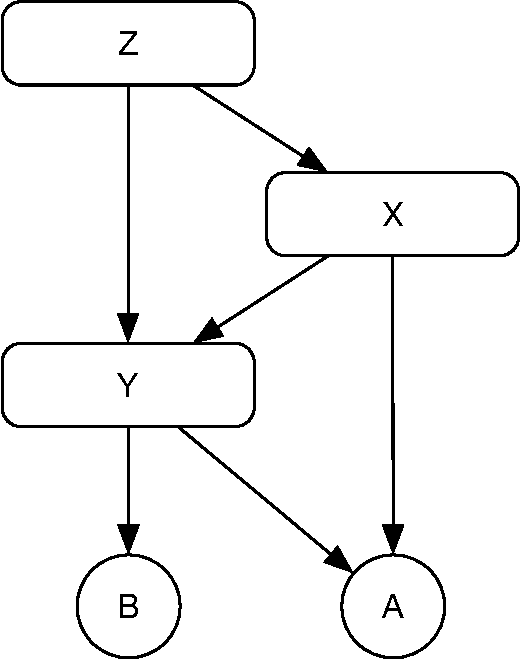
\includegraphics[width=1.5in]{dag}
\caption{A Simple Directed Acyclic Graph (DAG)}
\label{dag}
\end{wrapfigure}

Figure~\ref{dag} at right shows this very arrangement of these chains and patterns. In the computer science world, this kind of structure is known as a {\it Directed Acyclic Graph} or {\it DAG}.  It's a {\it graph} because every object is connected to other objects with lines called {\it edges}.  It is {\it directed} because there is a clear relationship between parents and children: that is, the edges are arrows indicating who the child is.  It's {\it acyclic} because no child can be its own ancestor: you can't have loops (or ``cycles'').  That is, all edges are pointing {\it down}.

You don't have to start playing at Chain Z.  You could instead choose to start playing at (say) Chain Y, and so Z and X would both just be ignored.  Seq calls the node that you're starting playing at the {\bf Root} of the current sequence (even if it itself has parents).

\paragraph{Seq Terminology}

Seq's sequences are DAGs built out of basic musical building blocks (step sequences, chunks of MIDI, etc.), and objects which group other building blocks into subsequences (including grouping other subsequences together).  All these objects, both basic and grouping, are know as {\bf motifs}.  Thus (to use the LM-1's terminology) both individual step sequence patterns and pattern chains are represented as kinds of motifs.  One motif is designated the {\bf root motif}, and is the start point when playing.  Motifs which group other motifs are known as the {\bf parents} of those {\bf children}.  

When you're editing a Motif, you'll be shown the {\bf Motif Display} and, to its right, various {\bf Inspectors} to modify the features of the Motif and how it manages its children (if it has them).  All your Motifs are collected into one group, called the {\bf Motif List}.

\paragraph{Macros and Parameterization}

Seq has two more powerful tricks up its sleeve, but neither of them is necessary to understand in order to use Seq: thus they are discussed at the end of the manual.

First, you can encapsulate an entire sequence into a single motif called a {\bf Macro}.  This allows you to use one sequence as an element to be called from another sequence.  Macros can also be set up to have their own children, so the encapsulated sequence can call motifs outside, in the outer sequence: this allows you to create Macros which are essentially pattern templates.  For more information on Macros, see Section~\ref{macros}.

Second, a great many of the features in motifs are {\bf parameterizable}.  This means you can attach them to {\bf parameters} in the motif itself, which can in turn be changed by the motif's parents or ancestors.  This allows a parent to automatically change a variety of features in its children or descendants.  For example, a parent could use a low-frequency envelope to change the pitch of certain notes in one of its children.  Parameters can also be changed with Control Change (CC) messages from external controllers, and parameters can also be used to send out many different kinds of MIDI messages, including CC, NRPN, and so on.  Parameterization is a complex  subject: for more information, see Section~\ref{parameters}.

\paragraph{Where We're Going with Seq}

Seq's sequence structure is very amenable to customization and automated modification.  Our ultimate goal is to ask what kinds of machine learning, optimization, or search techniques we could add to Seq to convert it into a {\bf co-creative tool} for the composer, that is, a tool that works with the composer, bouncing ideas back and forth, to produce a song.  We have previous experience in tools of this sort (see Sean Luke's {\bf Edisyn} for example).  But before we get to doing stuff like that, we have to get Seq finished.

\clearpage\section{The User Interface}

\begin{figure}[b]
\centering
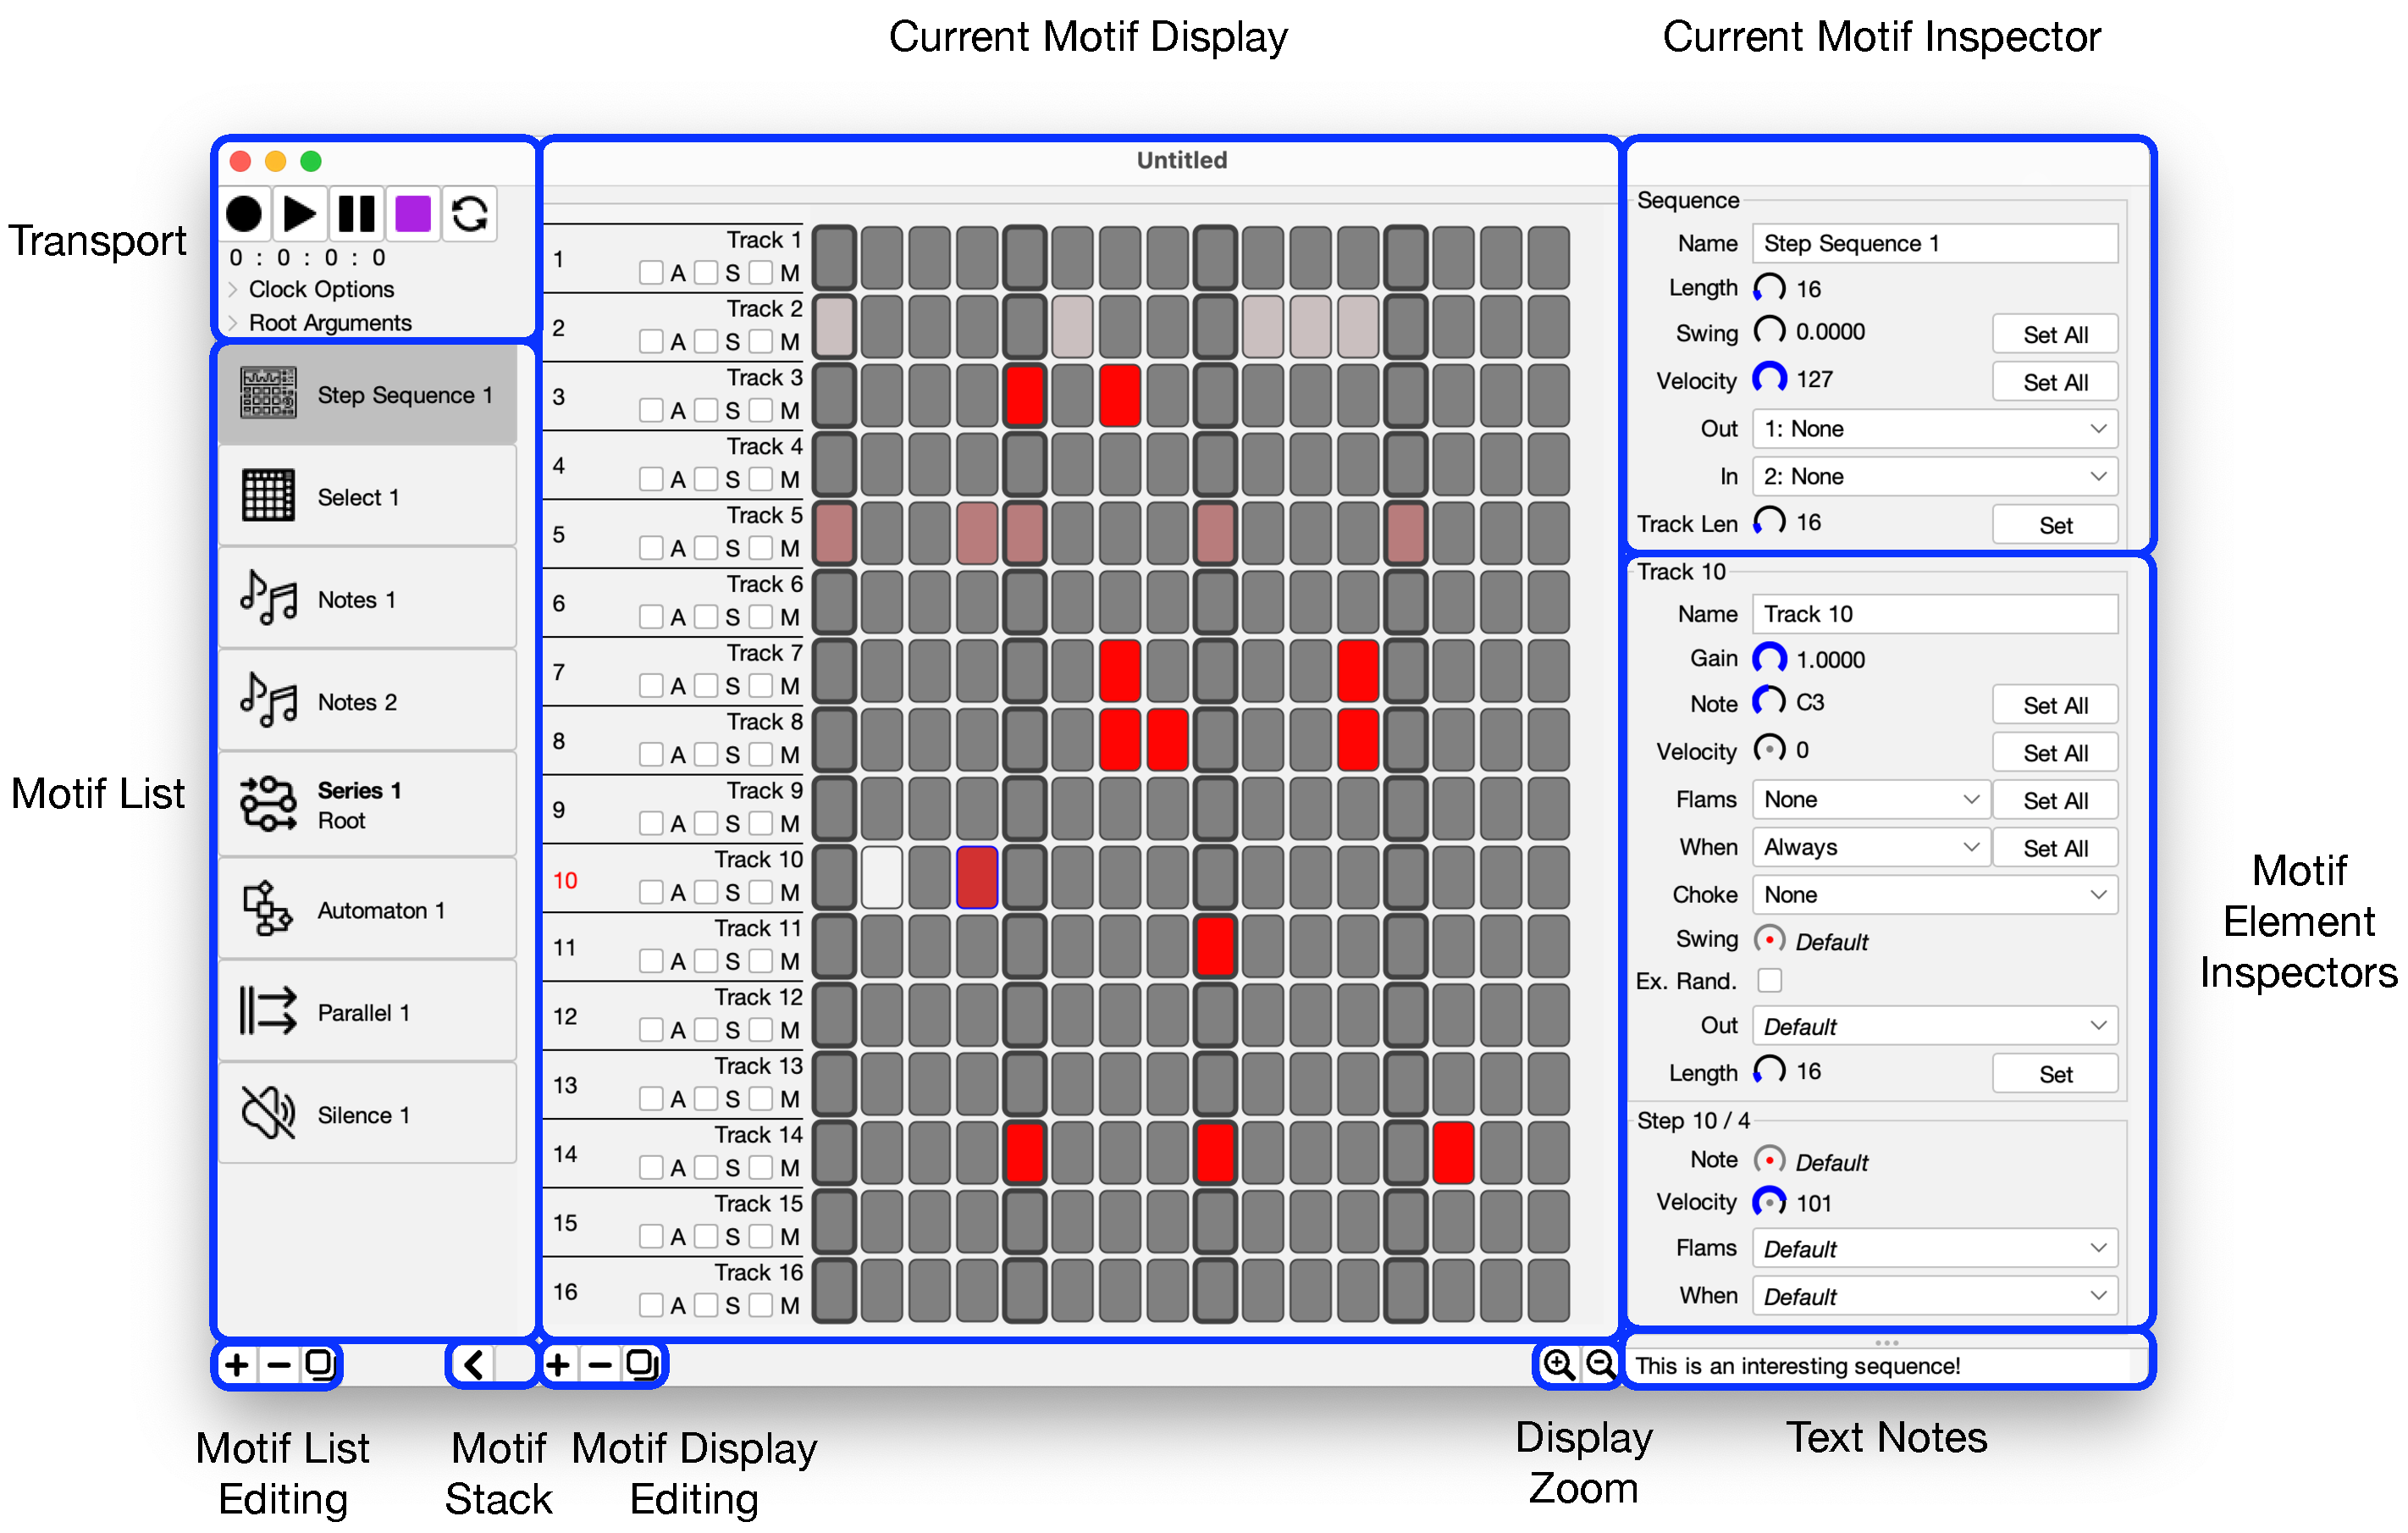
\includegraphics[width=6.5in]{MotifDisplay.pdf}
\caption{Seq graphical interface elements.}
\label{gui}
\end{figure}

Seq is organized with a single window, shown in Figure~\ref{gui}.  At top left is the {\bf Transport}, which contains the record, play, pause, stop, and loop buttons, plus the current time clock in ticks, beats, measures, and parts.  The Below the transport are two expandable regions for {\bf Clock Options} and for {\bf Root Arguments}.

Below the Transport is the {\bf Motif List}.  This is a scrollable list of every motif you have added to your sequence.  Below the Motif List are the {\bf Motif Editing Buttons} to add, remove, and duplicate motifs in the list; as well as the {\bf Motif Stack Buttons}, which let you return to previously visited motifs in order.

In the center of the window is the {\bf Current Motif Display}.  This shows the selected motif and lets you edit it.  Different motifs have different displays.  The one shown in Figure~\ref{gui} is a Step Sequence.  Below the Current Motif Display are are the {\bf Motif Display Editing Buttons}, which let you add to the display, delete from it, and copy elements in it; and the {\bf Display Zoom Buttons} which let you zoom in and out.  Different motifs have different options for these buttons.

At the right are the {\bf Inspectors}.  These are regions for editing the parameters of the current motif itself, and various elements in the motif.  At top right is the {\bf Current Motif Inspector}.  This holds editable features of the current motif.  For the Step Sequence, editor features include things such as the sequence name, length, degree of swing, etc.

Below the Current Motif Inspector are the {\bf Motif Element Inspectors}.  Different motifs have different kinds of elements, so a variety of things may appear here.  In this example, there is an inspector for the features of the currently selected Track (Track 3\,---notice this track's number is highlighted in red).  Below it is an inspector for the features of the currently selected step in this track (Step 7 of Track 3).  

Below the Inspectors is a resizable region for {\bf Text Notes} for each Motif.

\paragraph{Dials}

\begin{wrapfigure}{r}{1in}
%\vspace{-1em}
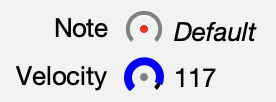
\includegraphics[width=1in]{smalldials}
\vspace{-2em}
\caption{Dials}
\label{dials}
\vspace{-1em}
\end{wrapfigure}

Most widgets are pretty standard in Seq.  But {\bf dials} require a little explanation.    A dial (usually) sets a numerical value: you set it by clicking on the dial proper and dragging up or down.  The dial then shows the numerical value to its right.   For example, the {\it Velocity} dial at right is set to 117.  

Some dials can be set to {\bf special values}.  These dials will have a little gray dot in the center of them (as was the case for the Velocity dial).  Sometimes there is only one special value.  If you double-click on the dial, it will automatically be set to this special value. If there are more than one special value, when you double-click on the dial, a menu will pop up to let you choose the special value you want.  If a special value is set, it is shown in {\it italics} and the little gray dot turns red.    For example, the {\it Note} dial  has been set to the special value {\it Default}.

If a dial has no special values available, no dot will appear.


\subsection{The Motif List\quad(and the Edit, Add, Motif, and File Menus)}

\begin{wrapfigure}{r}{1.5in}
\vspace{-2em}
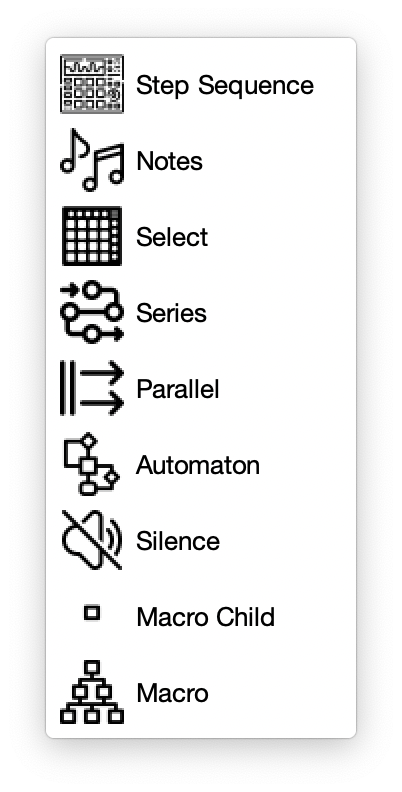
\includegraphics[width=1.5in]{motifs}
\vspace{-2em}
\caption{Available Motifs}
\label{motiflist}
\vspace{-1em}
\end{wrapfigure}

Each motif has a slot in the {\bf Motif List}, where it is shown with its current name.  You can rearrange the order of the motifs and select a new motif to display by clicking on it.  This will cause it to be displayed in the {\bf Current Motif Display}.  One motif is designated the {\bf Root Motif}, with the word {\bf Root} under the motif name.  This is the start point that will be played when the sequence is played.

When you select a motif, other motifs may appear in light blue.  These are the {\bf parents} of the motif, that is, the motifs which include the motif among their children.  Others are appear in pink: these are the {\bf children} of the motif.

When a motif is currently playing, its text will be highlighted in red.  Since a currently playing motif may also be playing its children, multiple motifs may appear in red at the same time.  

If a motif is armed for recording, it will appear with a little red circle before it.

Below the Motif List are the {\bf Motif List Editing Buttons}, which let you add new motifs to the list, delete them, and copy them.   Most importantly, clicking the ``\(+\)'' button will pop up the a {\bf List of Available Motifs}, as shown at right in Figure~\ref{motiflist}.  Select a motif and a new one will appear in the Motif List.   You can also choose the same motifs from the {\bf Add Menu}.

Also below the Motif List are the {\bf Motif Stack Buttons}.  When you select a motif, the current motif display changes to reflect the newly selected motif.  The previously selected motif is pushed on the stack.  You can go back to previous motifs by pressing the ``\(<\)'' button, and return to later selected motifs with the ``\(>\)'' button.  These buttons only appear if there is a motif to go back (or forward) to.

\paragraph{Motif Menu}

The Motif Menu has several options.  

	\begin{itemize}
	\item You can {\bf set the Root Motif} to the currently selected motif.  
	\item You can {\bf automatically set} motifs to be the the Root Motif whenever you select them.  
	\item You can {\bf Sort Motifs}, which organizes motifs so that children appear lower in the list than their parents.  
	\item You specify which kind of Motif is the {\bf initial one displayed} when Seq launches.
	\item You can change the motif buttons to a {\bf smaller size}.
	\item You can set things such that {\bf arming a motif} automatically disarms all the others.  If your Motif (notably Notes) is set to automatically arm itself when first created, this will also disarm the others.
	\item You can {\bf disarm all motifs} so that they no longer record MIDI.  This is useful if you've forgotten which ones you've armed so far.
	\end{itemize}

\paragraph{File Menu}
The File Menu allows you to load and save sequences and to clear the existing sequence and restart with a new one.  You can also {\bf Export} the sequence starting at the Root Motif, discarding all motifs that are not its children nor descendants.  Finally, you can {\bf Merge} another sequence into the current one: this adds to the current sequence copies of all the Motifs in the other sequence.

Seq can also load Type 1 and Type 2 MIDI files via {\bf Load MIDI File...}.  If the MIDI file has multiple tracks, or a single track with multiple channels, Seq will load the file as multiple Notes Motifs, with a Parallel Motif as their common parent. Otherwise, it will load the file into a single Notes Motif.  We will discuss the Notes and Parallel Motifs later.

\paragraph{Edit Menu}
The Edit Menu largely concerns itself with {\bf Undo} and {\bf Redo}.  However Undo works differently than you're used to: only structural changes are undone.  If you change a parameter, it's not undoable.  However you can add an undo point prior to the parameter change by choosing {\bf Checkpoint} before making the change.


\subsection{The Transport\quad (and the MIDI Menu)}

The Transport is how you play the sequence or start recording incoming MIDI.  The transport has a Record, Play, Pause, and Stop Button, as well as a Loop Toggle.  Buttons are highlighted in colors to indicate the current playing state.  Press the {\bf Play} button to start playing, and press {\bf Stop} to stop playing.  Press the {\bf Record} button to start recording.  The {\bf Loop Toggle} loops when playing: when the sequence has ended, it will start playing again.

The {\bf Fast Forward} button allows you to jump forward in time.  When you press it, Seq will ask you what time to fast forward to, and then will play the entire sequence at high speed (not outputting any MIDI) until Seq reaches the desired timestamp.\footnote{In a normal sequencer, you can just jump to a spot in the sequence because they are just a list of notes: but Seq's sequences can involve randomness and external external MIDI control which changes what notes are output, so it can't do that.}  At that point Seq will {\it pause} the sequence and the Fast Forward button will turn into a {\bf Pause} toggle button.  When you press the Pause button to resume playing the sequence, Seq will continue playing normally. 

The {\bf Pause} button also is available to pause or resume the sequence during normal playing or recording.

\begin{wrapfigure}{r}{1.5in}
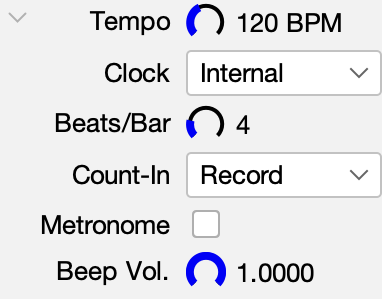
\includegraphics[width=1.5in]{clock}
\caption{Clock Options}
\label{clockoptions}
\end{wrapfigure}

When you start playing the sequence, play commences with the {\bf Root Motif}.  If the Root has parent motifs, they are ignored and not played.  

Recording only has an effect on certain Motifs, such as the {\bf Notes} motif, when they are armed.  Otherwise it acts just like playing for all other Motifs.

Below the Transport buttons is the {\bf Clock}, which shows the current play time in (right to left) ticks (192 ticks per beat), beats, measures, and parts (256 measures per part).  To the left of the clock is a small dot.  This dot will light up momentarily when Seq receives MIDI information (other than Note Off) from any of its currently registered devices and channels.

Below the clock are two expandable regions: the {\bf Clock Options} and the {\bf Root Arguments}.  The Clock Options include the tempo, whether the clock is Internal or External, the number of beats per measure, whether the metronome plays for recording,  for recording and playing, or for none; whether a count-in is provided for recording, for recording and playing, or for none; and the metronome volume and pitch.  Thee settings of some of these elements are stored with your Sequence; others persist in the application's preferences.

We'll discuss the Root Arguments later in Section~\ref{parameters}.  However we mention one item here: the {\bf Random Seed}.  This is the seed of the random number generator used by Seq when playing, and the generator is always reset to that seed each time we play again.  That way the sequence will always be deterministic.  The seed is saved with the Sequence when you write it to a file, but new Sequences get new random seeds. You can always change this seed to cause the sequence's random choices to be different.

\paragraph{MIDI Menu}

The MIDI Menu is where you set up MIDI to play and record.  First, you with {\bf Set MIDI Devices}, you can set up to 16 {\bf Outputs} and up to four {\bf Inputs} in your patch.  Each Input or Output is a combination of a MIDI Device and a Channel.  Once you have set up an input or output. it appears as an option in device selectors for Motifs which input or output MIDI.  Inputs and Outputs also have {\bf Nicknames}.  If you give an Input or Output a Nickname, the Nickname will appear in the selectors for various Features instead of the device name.  You get rid a Nickname by deleting the text in its text box.

When you select {\it Set} to save your choices, the Inputs and Outputs are saved not only with your patch, but also to global preferences so you next time you create a patch they'll be set by default.  You can optionally select {\it Reload}, which reloads the Inputs and Outputs from your patch, clearing the changes you just made.  If you load a patch, its current Inputs and Outputs will be loaded, overriding your defaults.

You can also {\bf Panic}.  This sends an {\bf All Sounds Off} and an {\bf All Notes Off} to every setup device in order to quiet MIDI devices with stuck notes.

Finally, you can {\bf Log MIDI} to a file or generate a collection of {\bf Notes} objects from it.  If you start logging, then the next time you press Play, Seq will start logging a copy of all of its MIDI output.  The logging stops when you press Stop.  At that point, the logged MIDI is emitted to a single MIDI file, or broken out per-device to separate MIDI files,\footnote{When emitted to a single file, each device is written out as a separate channel.  Some DAWs, such as Ableton, cannot read multi-channel MIDI files; hence the separate MIDI file option.}, or to a collection of Notes motifs, one for each device used.  If more than one Notes is created, they will all be grouped under a single {\bf Parallel} motif: if you play that Parallel as root, you'll hear the same music again.  For more on Notes and Parallel, see Sections~\ref{notesmotif} and~\ref{parallelmotif} respectively.

\subsection{The Current Motif Display\quad (and the Options and Per-Motif Menus)}

The current motif display varies depending on which motif you have selected in the Motif List.  Different motifs have different displays according to the nature of their data.  We'll discuss different motifs and their displays later in Section~\ref{motifs}.  

 Below the Current Motif Display are the {\bf Motif Display Editing Buttons}.  These vary depending on motifs and their need, though you might commonly see a button for adding elements, deleting them, or copying them.  For example, in Figure~\ref{gui}, the Step Sequencer display has a ``\(+\)'' for adding a Track, a ``\(-\)'' for deleting the current track, and a button for duplicating the current track.

Also below the Current Motif Display are the {\bf Display Zoom} buttons.  These zoom the display in and out and again are only appropriate for certain motifs (notably the Step Sequencer motif).

\paragraph{The Per-Motif Menus}  Some motifs have their own dedicated menu which appears only when that motif is selected.  These menus will be discussed with the motifs proper in Section~\ref{motifs}.

\paragraph{The Options Menu}  This contains miscellaneous sequencer options.  {\bf Show Tooltips} toggles whether you want tooltips popping up everywhere.  This option is remembered after you quit and restart Seq.  {\bf  New Random Number Generator} gives Seq a random number generator with a new random sequence.  And if {\bf New Generator Each Play} is check, Seq produces a new random number generator each time you press the Play or Record buttons: this is also remembered after you restart Seq.  These last two menu items require some explanation.

Each sequence has a random number generator, which produces a stream of random numbers used whenever Seq has to roll the dice for something.  Each time you make a new sequence, it is given its own  unique random number generator, which is saved with the sequence.  When you stop and replay the sequence, this generator is reset so you'll always have the same random choices made and thus will have the same sequence.

Normally this is desirable.  But what if you don't like the stream of numbers you were given, and want a new random generator?  Select "New Random Number Generator", and you'll get a new one.  You can go back to the old one with {\bf Undo}.  If you save your sequence, it'll be saved with to use the new generator.

Note that if you change your sequence such that elements that draw random numbers are added, removed, or moved, you'll probably change the effect of the sequence on all the later random elements anyway.  So don't expect the random series to be the same after you've made significant changed to your sequence.

\subsection{The Inspectors and Text Notes}

Each motif, and each element contained inside a motif, has an {\bf Inspector}.  An Inspector is a labelled list of every editable feature of the motif or element.  Inspectors appear in the column at the far right of the window.  Inspectors change a the Current Motif, or elements selected within the Current Motif, change.

At top right is the {\bf Current Motif Inspector}.  This is, unsurprisingly, the Inspector for the editable features of the Current Motif.  Different motifs will have different available features, though they will all have at least {\it one} feature: the Motif's {\bf Name}.  By default the name is something boring like ``Automaton 1'', but you can rename it to anything you want.

Some Motifs also have {\bf Parameters} their child motifs can refer to.  Each of these parameters can be custom named, and the parameter names appear as an expandable region in the Current Motif inspector.  We'll discuss parameters later in Section~\ref{parameters}.

Below the Current Motif Inspector may appear {\bf Element Inspectors}.  For example, in Figure~\ref{gui}, below the Step Sequence inspector appear Inspectors for the currently selected Track in the Sequence, and for the currently selected Step in the Track.  Many Motifs have Element Inspectors, but they vary.  Motifs that hold Child Motifs typically show an Inspector for the currently selected Child, for example.

At bottom are {\bf Text Notes}.  You can resize this region and store all the notes you like, and they will be saved with each Motif.

\clearpage\section{The Motifs}
\label{motifs}

Excluding Macros and Macro Children, there are presently nine Motifs available in Seq:

\begin{itemize}
\item Three {\bf Basic (Note-Generating) Motifs}: Step Sequence, Notes, and Silence.  These do not have children Motifs.
\item Four {\bf Combination Motifs}: Series, Parallel, Automaton, and Select.  These have children Motifs.
\item One {\bf Parameter Modification Motif}: Modulation.  This has a single child Motif.
\item Two {\bf MIDI Effect Motifs}: Arpeggio and Filter.  These have a single child Motif each.
\end{itemize}

We'll be adding more Motifs in time.

\vspace{1em}

Motifs are played through once, and when they have finished playing they do not themselves loop, but rather signal to their parent that they are {\bf finished}.  The parent then decides what to do with them, such as play them again, or go on to play something else, or signal to {\it its parent} that it is finished, and so on.

You can loop the entire sequence\,---\,that is, loop the {\bf Root Motif}\,---\, by toggling the Loop button in the Transport prior to or during playback.

\clearpage
\begin{figure}[t]
\centering
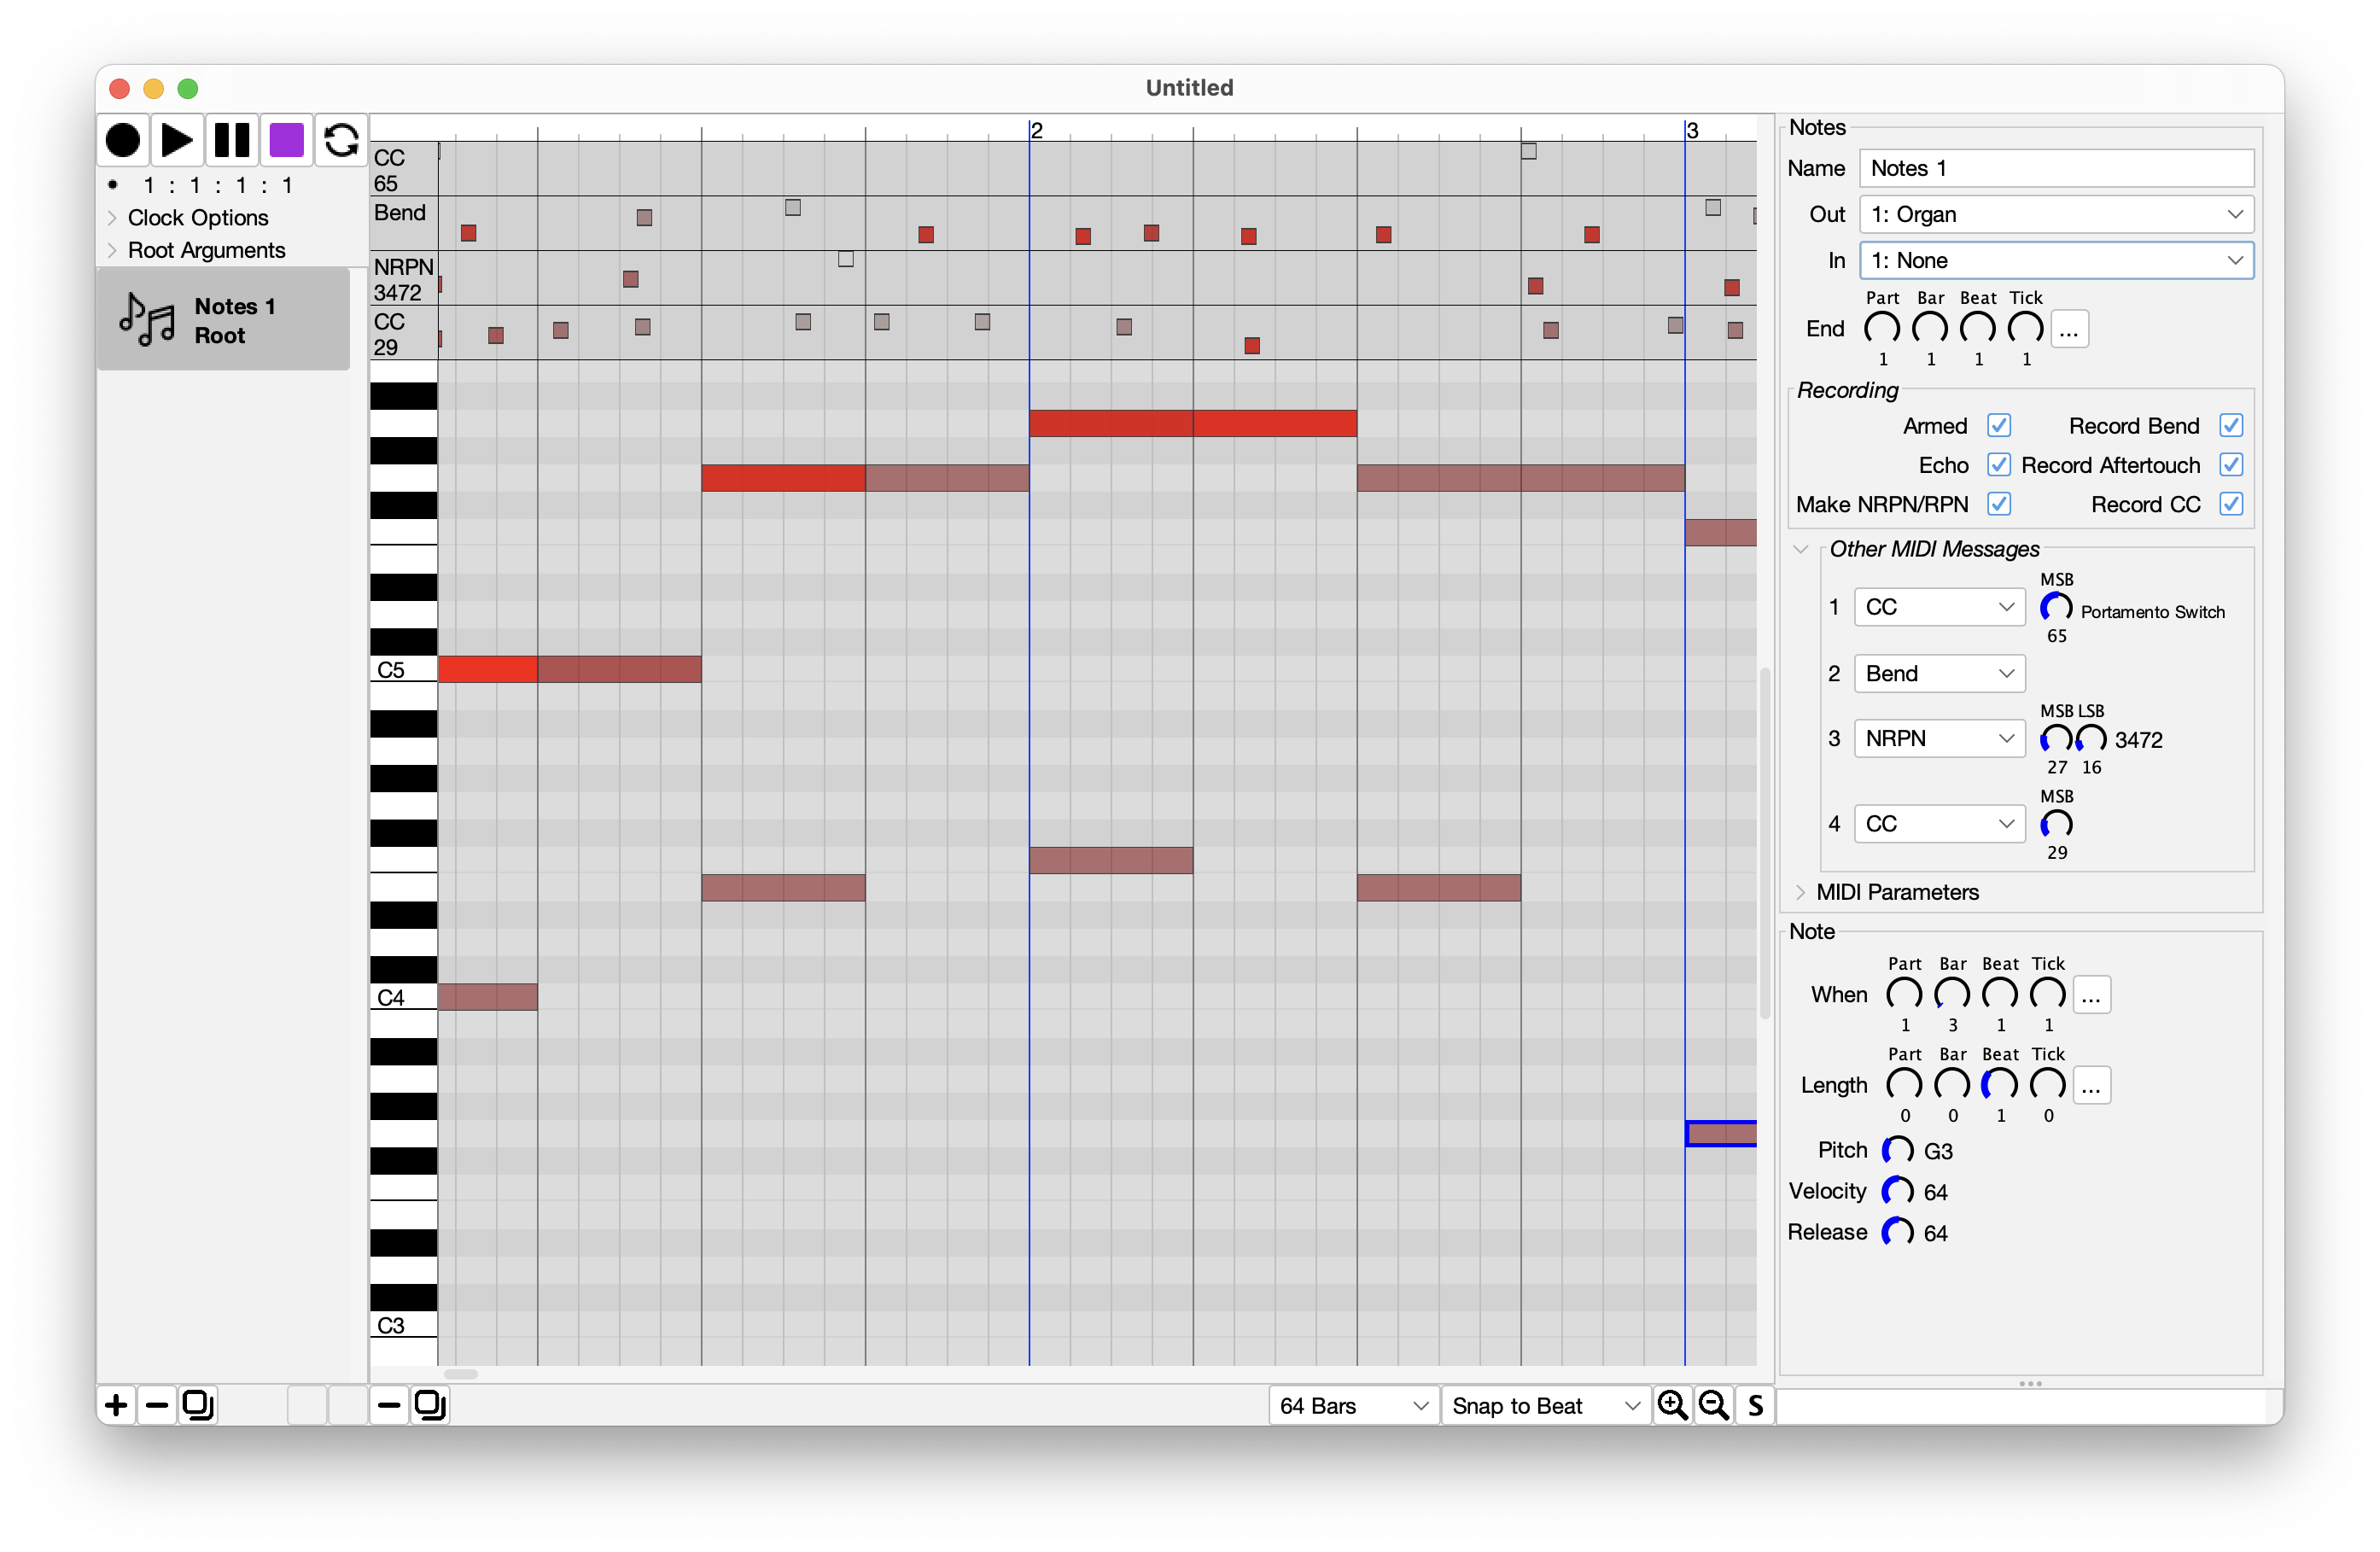
\includegraphics[alt={yo},width=6.5in]{Notes}
\vspace{-2em}
\caption{Notes Motif.}
\label{notes}
\end{figure}

\subsection{Notes}
\label{notesmotif}
 
Notes is simply a collection of MIDI events: MIDI Notes, Pitch Bend events, Control Change (CC) events, Program Change (CC) events NRPN/RPN events, and Aftertouch Events.  Notes are not stored as MIDI Note On/Note Off, but as entire notes with an onset, pitch, velocity, length, and release velocity.   Other events are simply stored as their time stamp and value.  

Like other Motifs, you can give your Notes a {\bf Name} in the Notes Inspector.  

\paragraph{The Note and Event Displays}

Notes are displayed using a {\bf piano player roll} with scroll bars: the Y axis is pitch (with a little keyboard display at left to help you out) and the X axis is time.  The color of the note is its {\bf velocity}.  

Other events are {\bf optionally displayed} above the piano player roll.  In the image above, you can see the time-stream of four such events. You select up to four event types to display with the {\bf Non-Note Display} disclosure panel in the Notes Inspector at right.  You can change the height of the event displays with {\bf Parameter Height}.

The color of a non-note event is (at present) its {\bf value}.  The value is also shown with the {\it vertical position} of the event.  Pitch Bend is a special case: although it has a large range (\(-8192\) to \(+8191\)), very often subtle difference near 0 are important but can't be seen in the display due to resolution.  By default Seq displays Pitch Bend warped (using square root), so values near 0 take up lots of space and large values take up rather little space.  If you don't like this, you can turn it off by unchecking {\bf Warped Pitch Bend} in the Non-Note Display disclosure panel.  (Polyphonic Aftertouch is also a special case: its color reflects its pitch, not value.)

 You can change the {\bf maximum length of time} of the piano player roll with a pop-up menu at the bottom of the window, anywhere from 64 to 65536 bars.  Making the length longer doesn't consume more resources, and it's not slower.  But it will make horizontal scrolling more annoying.  So you'd like to keep it reasonably short when possible.

You can {\bf zoom} the piano player roll in and out with the magnifying glass buttons at the bottom of the window.

At the top of the display is the {\bf Ruler}.  Depending on the zoom amount, will display ticks for Bars, Beats, and 16th notes.  It will also show numbers for Bars.

\paragraph{Creating Notes and Events}

The create a note or an event, just double click in its region where you want it to be.  The velocity and release velocity of the note will be set to the {\bf Initial Velocity} and {\bf Initial Release Velocity} respectively, found under the {\bf Note Editing} disclosure panel in the inspector.

The position of the note or event, and the size of the note, are governed by the {\bf snap} value, which you can set via a pop-up menu at the bottom of the window:

\begin{itemize}
\item {\bf No Snap}\qquad The note/event onset will be placed right where you clicked.  The note will be a quarter note (a beat).
\item {\bf Snap to/by 64th}\qquad The note/event onset will be placed at the nearest 64th note.  The note will be a 64th note.
\item {\bf Snap to/by 16th}\qquad The note/event onset will be placed at the nearest 16th note.  The note will be a 16th note.
\item {\bf Snap to/by Triplet}\qquad The note/event onset will be placed at the nearest triplet.  The note will be a triplet.
\item {\bf Snap to/by Beat}\qquad The note/event onset will be placed at the nearest quarter note (beat).  The note will be a quarter note.
\end{itemize}

\paragraph{Selecting and Adjusting Notes}

You can select a note by clicking on it.  It will get a highlighted selection border in blue.  Once you have selected a note, you can drag it to change its pitch or time.  You can also change the length of the note by clicking and dragging the note near its right end.

You can also select multiple notes by clicking on the display and dragging a rubber-band around them.  

If you hold down the {\bf shift key} you can add and remove notes to your selection by clicking them or rubber-band dragging around them.  You can do the same by {\bf right clicking}.

If you hold down the {\bf option} or {\bf alt} key while dragging, or drag with the {\bf middle mouse button}, then the selected notes will change in pitch but not in time.

If you have selected only one note, its Inspector will appear, and you can change its timestamp, length, pitch, velocity, and release velocity manually.

When you change the time or length of a note and you have {\bf Snap To} turned on (see the pop-up menu at the bottom of the screen), it will {\bf snap} to the nearest 64th note, 16th note, triplet, or beat.  If instead you have {\bf Snap By} turned on, it will {\bf jump} forward or backward by one 64th note, 16th note, triplet, or beat in distance.

If you have lost your notes, just play the {\bf Find Notes} button (the {\bf ``F''} at the bottom of the window, and the piano player roll will scroll to show your selected notes, or any notes at all (if you have nothing selected).

Selected notes can also be moved by through the {\bf Up, Down, Left, and Right} menus and their corresponding keystrokes. 

\paragraph{Selecting and Adjusting Non-Note Events}

Just like notes, you can select events by clicking on them, rubber-band selecting them (the rubber band will be a 1-dimensional range, not two-dimensional), and using the {\bf shift key} or {\bf right-click} in the same way.  And if you have selected only one event, its Inspector will appear allowing you to change it more precisely.

You probably don't want to change both the time and value of a non-note event, so there are some constraints to help you out.  When you drag a non-note event what happens depends on what keys you are holding down:

\begin{itemize}
\item {\bf [Nothing]}\qquad Adjusts value but not time.
\item {\bf Option/Alt or Middle-Click}\qquad Adjusts time but not value.
\item {\bf Command/Windows}\qquad Adjusts both time and value.
\item {\bf Control}\qquad If adjusting value, all selected events are set to the same value.
\end{itemize}        

Adjusting non-note Events in time follow the same {\bf Snap To} and {\bf Snap By} rules as for Notes.  And the {\bf Show Notes} facility also works for selected events.

Selected Events can also be moved by through the {\bf Up, Down, Left, and Right} menus and their corresponding keystrokes. 

\paragraph{Deleting and Duplicating}

You can delete your selection with the {\bf Delete Button} (the minus sign) at the bottom of the window.  You can duplicate your selection with the {\bf Duplicate Button} next to it.  You can also delete from an option in the {\bf Notes Menu}  

\paragraph{Playing Notes (and other Events)}

When Notes is played, it plays through and emits all its events in order exactly once, then stops.  You can optionally set a {\bf Start} point and an {\bf End} point in the Inspector.  Play will commence at the Start point, and will end after the End point, or after the last note or event in the sequence, whichever is later.  Start can obviously be equal to or after End: in this case, play commences at start and ends as soon as the last note or event is over.

All notes and events are emitted out the same MIDI output specified by the {\bf Out} in the Notes Inspector.

\paragraph{Recording Notes (and other Events)}

You can record notes from MIDI into the Notes.  To do this you must first {\bf Arm} the Notes: check the {\bf Armed} checkbox in the Notes Inspector.  Then start recording by pressing the record button.  Recording will only start once it's the Notes's time to play.  Notes will record MIDI from the MIDI Input specified by the {\bf In} in the Notes Inspector.

If you check the {\bf Echo} checkbox in the Notes Inspector, Notes will play to its Output all the notes it receives at its Input while recording.  Note that whichever Notes motif was most recently open will control the Echo settings.

In the {\bf Recording} disclosure panel there are a number of recording options.   First, of you can specify the {\bf Integration} of the notes and events after they are recorded:

\begin{itemize}
\item {\bf Replace} means to delete all existing events and replace them with the newly recorded ones.
\item {\bf Replace/Trim} is the same, except that time is trimmed from the start so that the first recorded note or event starts at the first timestep.  This is probably best if you also quantized.
\item {\bf Merge} means to simply add the new events to the existing ones (mixing them in).
\end{itemize}

Next, if you check the {\bf Record Bend}, {\bf Record Aftertouch}, or {\bf Record CC} checkboxes, Notes will record these events: otherwise it will ignore and discard them while recording.   And if you check the {\bf Make NRPN/RPN} checkbox, Notes will attempt to build NRPN or RPN parameters as it receives them.  NRPN and RPN parameters are made up of collections of CC messages, so if those CC messages are used to build a parameter, the CC messages will not be recorded as CC messages but as NRPN or RPN.  

Other recording options deal with automatic quantization.  You can turn {\bf Quantize} on for notes, instruct it to also {\bf Quantize Note Ends} and to {\bf Quantize Non-Note Events} (like pitch bend or CC), and tell it to {\bf Quantize To} a certain resolution.  There also is a mysterious {\bf Quantize Bias} knob.  Normally Quantize works by rounding your note to the nearest resolution point, before or after.  By adjusting the Quantize Bias knob you can push Quantize to more likely round to the note before or to the note after.  This is useful because as humans we each have a different tendency to either play too early or too late, and can set the Quantize Bias knob to adjust for our own nature.

Recorded notes appear while recording.  However recorded non-note events will not appear until after recording is finished, simply because there can be too many of them to draw efficiently.

\paragraph{The Notes Menu} Notes has a number of items under its menu.  Many of these items are applied to either all events or to a subset of them, depending on how you have selected notes or non-note events: 

\begin{itemize}
\item {\bf Selecting Notes or Events} will cause the menu item to only apply to the selection.
\item {\bf Setting a Range in the Ruler}.  You can drag in the ruler to create a range of time.  Menu items will apply to {\it all events}, both note and non-note events, within that range.  You can deactivate the ruler range by clicking in the ruler.  Note that the ruler range does not effect Deletion or Copying: they require selection.
\item {\bf All Events and Notes}.  If nothing is selected, and there is no ruler range set, then the menu item will apply to all notes.
\end{itemize}

\noindent The menu items are:

\begin{itemize}

%\item{\bf Load MIDI File...}\quad will load MIDI data from a MIDI file, replacing the existing data.

\item{\bf Select All Notes}\quad selects all notes.

\item{\bf Cut} and {\bf Copy} do what you expect.  They cut/copy either the selected events, or all events which fall inside the Ruler range.

\item {\bf Paste}\quad also does what you expect: it pastes the cut/copied notes, merging them into the existing notes.  But where do the Pasted events go?  If you have selected a range in the Ruler, Paste will paste its events starting at the beginning of that range.  If you have selected notes or events, Paste will paste its events immediately after the selection.  If no notes or events are selected, and the ruler has no range, Paste will paste its events right where they were cut or copied.  This is intentional, though it might confusing as they'd be on top of their previous notes/events.

Note that you can cut/copy from one Notes motif and Paste into a different one.

\item {\bf Paste/Replace}\quad is just like Paste, except that the selected events, or those in the Ruler range, will be deleted and replaced with the pasted events.

\item {\bf Replicate}\quad copies the selected or range events and places that copy in its own new Notes motif.  The events are trimmed so that they start at timestep 1..

\item{\bf Quantize...}\quad gives options for quantizing all or a selection/ruler range of your notes or event data. 

 A note about  the {\bf quantization bias}.  What is this?  Normally quantizers just round the notes up or down to the nearest quantized position, but this is often wrong.  As a human, you may tend to play more notes early than late (or vice versa), resulting in an error distribution which is {\it ought} to favor the earlier quantized positions more than the later one (or vice versa).  You can set the bias to match your personal tendencies.

\item{\bf Stretch Time...}\quad stretches the time of all of your data or the selection/ruler range.

\item{\bf Trim Blank Time from Start}\quad removes empty time from the start of your data.  Your first event will start at timestep 1 in the Notes.

\item{\bf Randomize Time...}\quad gives options for adding noise to the onset and optionally the duration of all of your data or the selection/ruler range.

\item{\bf Set Velocity...}\quad lets you set the velocity of all notes or those in the selection/ruler range.

\item{\bf Randomize Velocity...}\quad gives options for adding noise to the velocity of all notes or those in the selection/ruler range.

\item{\bf Interpolate...}\quad adds additional non-note events in-between the selected events to gradually shift the event value from one to the other.  You can interpolate among more than just two events.  You can't interpolate notes.

\item{\bf Delete Selection}\quad deletes the selected events.  Note that this does {\it not} delete events within the ruler range.

\item{\bf Filter...}\quad gives options for filtering out (deleting) notes, bend data, CC data, RPN and NRPN data, or aftertouch data.  Since selection is applied to a single kind of data, Filter is really is only appropriate for filtering all data, or data within the ruler range (not selection).

\item{\bf Move to Top}\quad sets the selected notes so that they display on top of other notes.

\item{\bf Send to Back}\quad sets the selected notes so that they display behind other notes.

\item{\bf Arm New Notes Motifs}\quad sets it so that new Notes Motifs will automatically be armed (or not).

\end{itemize}

\paragraph{Parameterization}

Several Notes features (note velocities, release velocities, event values) can be {\bf Parameterized} by double-clicking on the dials.  If a note velocity or event value is parameterized, the note or event is displayed in gray-blue to indicate this.  For more on parameterization, see Section~\ref{parameters}, (\textbf{\textit{Parameterized Control of MIDI Data}}).

\clearpage

\begin{figure}[t]
\centering
\includegraphics[width=6.5in]{StepSequence}
\vspace{-2em}
\caption{Step Sequence Motif.}
\label{stepsequence}
\end{figure}

\subsection{Step Sequence}

Step Sequence is one of the most complex motifs, as it is a reasonably full-featured multitrack step sequencer.  Step Sequence defines a single multitrack pattern, which is played once and then declares it is finished.  The Step Sequence can have any number of Tracks, and each Track can have any number of Steps (and that number can vary from Track to Track).  By default the Step Sequence presents itself with 16 Tracks of 16 Steps.  

You select a Step by clicking on it.  This also selects the Step's Track.  You can also select a different Track (and its equivalent Step) by clicking on the Track Header (see below).  When you select a Step and Track, they will show their respective Inspectors at right below the primary Step Sequence Inspector.

If you triple-click on a Step, you will deselect all the Steps in its Track.

\paragraph{Defaults and Parameterization}

Several of the dials the Step Sequence's Tracks and Steps can be set to a fixed value or to {\bf Default}.  In a Step, Default means that instead of being fixed to a value, the dial defers to the Track's setting.  In a Track, Default means that instead of being fixed to a value, the dial defers to the Step Sequence's overall setting.

To set a dial to Default, double-click on it, and select {\it Default} from the resulting pop-up menu.  To set a Defaulted dial back to a fixed value, just change the dial.  You'll note that the pop-up menu has other values, such as Rand or Param 1 ... Param 8.  We'll discuss those in Section~\ref{parameters} ({\bf Parameterization}).  Don't set to those for now.  Furthermore, some menus don't have a Default, or no pop-up menu even appears: this means that the dial doesn't have a Default.  You can tell that a dial has a pop-up menu because it has a red or gray {\bf dot} in its center. 

\paragraph{Steps}

A Step is either {\bf off} (gray) or {\bf on}.  When on, the Step has a {\bf velocity} (volume), represented by a gradiated color between white and red.\footnote{Note that because MIDI interprets velocity=0 as a Note Off message, which we do not want, Seq will treat a velocity of 0 as a (very low) velocity of 1.} Each Step can also have its own {\bf Note Pitch}, its own number of {\bf Flams} (ratchets), and a declaration of {\bf When} (or perhaps better called {\it whether}) the Step plays when its time is up.  The When setting can be {\it always}, or it can play with some {\it probability}, or it can play with some {\it pattern}.  An example pattern is \textsf{O O X}, which means to play the first two times the Step Sequence is iterated, and then not play the third time, and then repeat. 

All four of these features (Note, Velocity, Flams, and When) also can be set to the special value {\bf Default}.   

Every fourth Step is bolded in the interface only for visual assistance.    The currently selected Step is outlined in blue.

\paragraph{Tracks}

A track is an iteration of Steps played one after another.  Even though tracks can have different numbers of steps, they will play their steps such that they all finish at the same time.

A Track has a {\bf Track Header} and then the list of Steps.  You can change the order of a Track in the list of Tracks by dragging its Track Header up or down.  A Track also has a {\bf Name}, which you can set in its Inspector,  Track Headers have three buttons: {\bf Learn (L), Solo (S),} and {\bf Mute (M)}.  If you select Mute, then that track will not play.  If you select Solo, then {\it only} that track will play.  If you select Learn, then the track is {\bf learning} its track note while playing.  This means that if you press a key, the track will use that key as its output {\bf Note}.     

You can add, delete, and duplicate tracks with the buttons at bottom.  You can also Zoom In and Zoom Out.  The currently selected Track has its track number highlighted in red.

Tracks have a number of features in their Inspectors, beyond their {\bf Name}.

All the Steps in a given Track play their MIDI out the same MIDI Out as specified by the Track.  By default this is set to the special value {\it Default}, meaning that the Track defers to the Sequence's global setting.  A track also has a {\bf Gain} which is multiplied against the velocities of its Steps to determine their final volume.  

A track also has a default {\bf Note}, {\bf Velocity}, number of {\bf Flams} and {\bf When} for its Steps.  By default Steps defer to these values, but you can of course change them on a per-Step basis.  You can also press {\bf Set All}, which causes all Steps to reset themselves to Default for that feature.

Each track also has up to one {\bf Choke Track}: when a Step in the Track is played, any playing sound in the Choke Track is immediately stopped (a MIDI Note Off is issued).  Tracks also have some degree of {\bf Swing} (syncopation).  A typical amount of swing would be about 30\% (if you wanted Swing), else 0\%.

A Track can be a member of the {\bf Exclusive Random Group} (or ``Ex. Rand.'').  When the Sequence is played, one and only one Track in the Exclusive Random Group is played; the others are hushed (independent of Mute settings).  The Track in question is selected at random. Tracks not in this group are not effected.

Finally, a track has a {\bf Length}, that is, the number of steps.  This is not set until the {\bf Set} button is pressed.

\paragraph{Euclidean Rhythms}

In 2004 Godfried Toussaint published a paper suggesting that large numbers of common rhythms worldwide could be automatically generated using Bjorklund's Algorithm, which is somewhat related to Euclid's Algorithm.  He called these {\bf Euclidean Rhythms}.  Bjorklund's Algorithm takes a track \(K\) steps long and attempts to fill it with \(N\) steps that are statistically evenly spaced from one another.  So there are two parameters, \(0 < N < K\).  Euclidean rhythms have since become all the rage.

Seq can fill a track with a Euclidean Rhythm with {\bf Euclid}.  You specify \(N\), the number of steps you want on (the rest will be off.  \(K\) is just the length of the track.  You can also {\bf Rotate} your Euclidean Rhythm to a new starting point  The Rhythm is generated when you press {\bf Set}.

\paragraph{The Step Sequence Inspector}

At top, the Step Sequence inspector defines the global settings for the Step Sequence.  There is its {\bf Name} of course.  After this there is the {\bf Duration}, that is, the length of time (in 16th notes) that this Step Sequence will take to complete.  For example, even if the Step Sequence is 16 steps long, if you set the Duration to 4, it'll run at the speed necessary to complete those 16 steps in one quarter note of time.  The default is of course 16: 16 steps in 4 quarter notes.

You can also set the default {\bf Swing}, {\bf Velocity}, and {\bf Out}, and Tracks will defer to these if set to {\it Default}.  The {\bf Track Length} indicates the initial number of Steps for newly added Tracks. Finally, {\bf In} specifies the MIDI Input to use when recording tracks.

\paragraph{Sequencing Things Other than Notes}

The Step Sequence inspector also has an option called {\bf Type}.  By default, this is set to ``Note'', but you can set it to other kinds of MIDI types, such as CC or NRPN.   This affects the meaning of the ``Note'' and ``Velocity'' dials, and also each step's Velocity coloring, as follows:

\begin{itemize}
\item {\bf Note}\qquad Nothing changes.
\item {\bf CC (Control Change)}\qquad ``Param'' represents the CC parameter.  ``Value'' represents the CC value.
\item {\bf Poly Aftertouch}\qquad ``Param'' represents the polyphonic aftertouch note.  ``Value'' represents the aftertouch value.
\item {\bf Channel Aftertouch}\qquad ``Param'' does nothing.  ``Value'' represents the CC value.
\item {\bf Pitch Bend}\qquad ``Param'' does nothing.  ``Value'' represents the MSB of the pitch bend value, and its ``LSB'' represents the LSB of the value .  The final pitch bend value, which ranges from -8192 to +8191, is defined as \(\text{\it MSB} \times 128 + \text{\it LSB} - 8192\). We recognize that Pitch Bend is defined in an inconvenient way.  We're working on it.
\item {\bf PC}\qquad ``Param'' does nothing.  ``Value'' represents the PC value.
\item {\bf NRPN}\qquad ``Param'' represents the MSB of the NRPN parameter, and its ``LSB'' represents the LSB of the parameter.   The final NRPN parameter, which ranges from 0 to 16383, is defined as \(\text{\it MSB} \times 128 + \text{\it LSB}\).  ``Value'' represents the MSB of the NRPN value, and its ``LSB'' represents the LSB of the value.  The final NRPN value, which ranges from 0 to 16383, is defined as \(\text{\it MSB} \times 128 + \text{\it LSB}\).  
\item {\bf RPN}\qquad Similar to NRPN.
\end{itemize}

\paragraph{The Menu}

The {\bf Step Sequence} menu allows you to use keystrokes make your away around the sequence ({\bf Up, Down, Left, Right}).  You can also {\bf Toggle} the selected step to be on or off.  And you can {\bf Rotate} all the steps in the selected track {\bf Left} or {\bf Right} by one step.

\ignore{
\paragraph{Recording a Step Sequence}

If you arm one or more Tracks, set their Notes, and set the Sequence's MIDI Input accordingly, then you can record in Notes to those tracks when you press Record on Seq.   You will find this easier if you turn on the metronome and if you set the Step Sequence to be the Root, so it records immediately.  Remember that if your Step Sequence motif is not a descendant of the Root, it will never be reached to do Recording.
}

\paragraph{Parameterization}

Several Step Sequence features (step velocities and pitches, swing, etc.) can be {\bf Parameterized} by double-clicking on the dials.  If a step's velocity is parameterized, the step is displayed in gray-blue to indicate this.  For more on parameterization, see Section~\ref{parameters}, (\textbf{\textit{Parameterized Control of MIDI Data}}).


\clearpage


\begin{figure}[t]
\centering
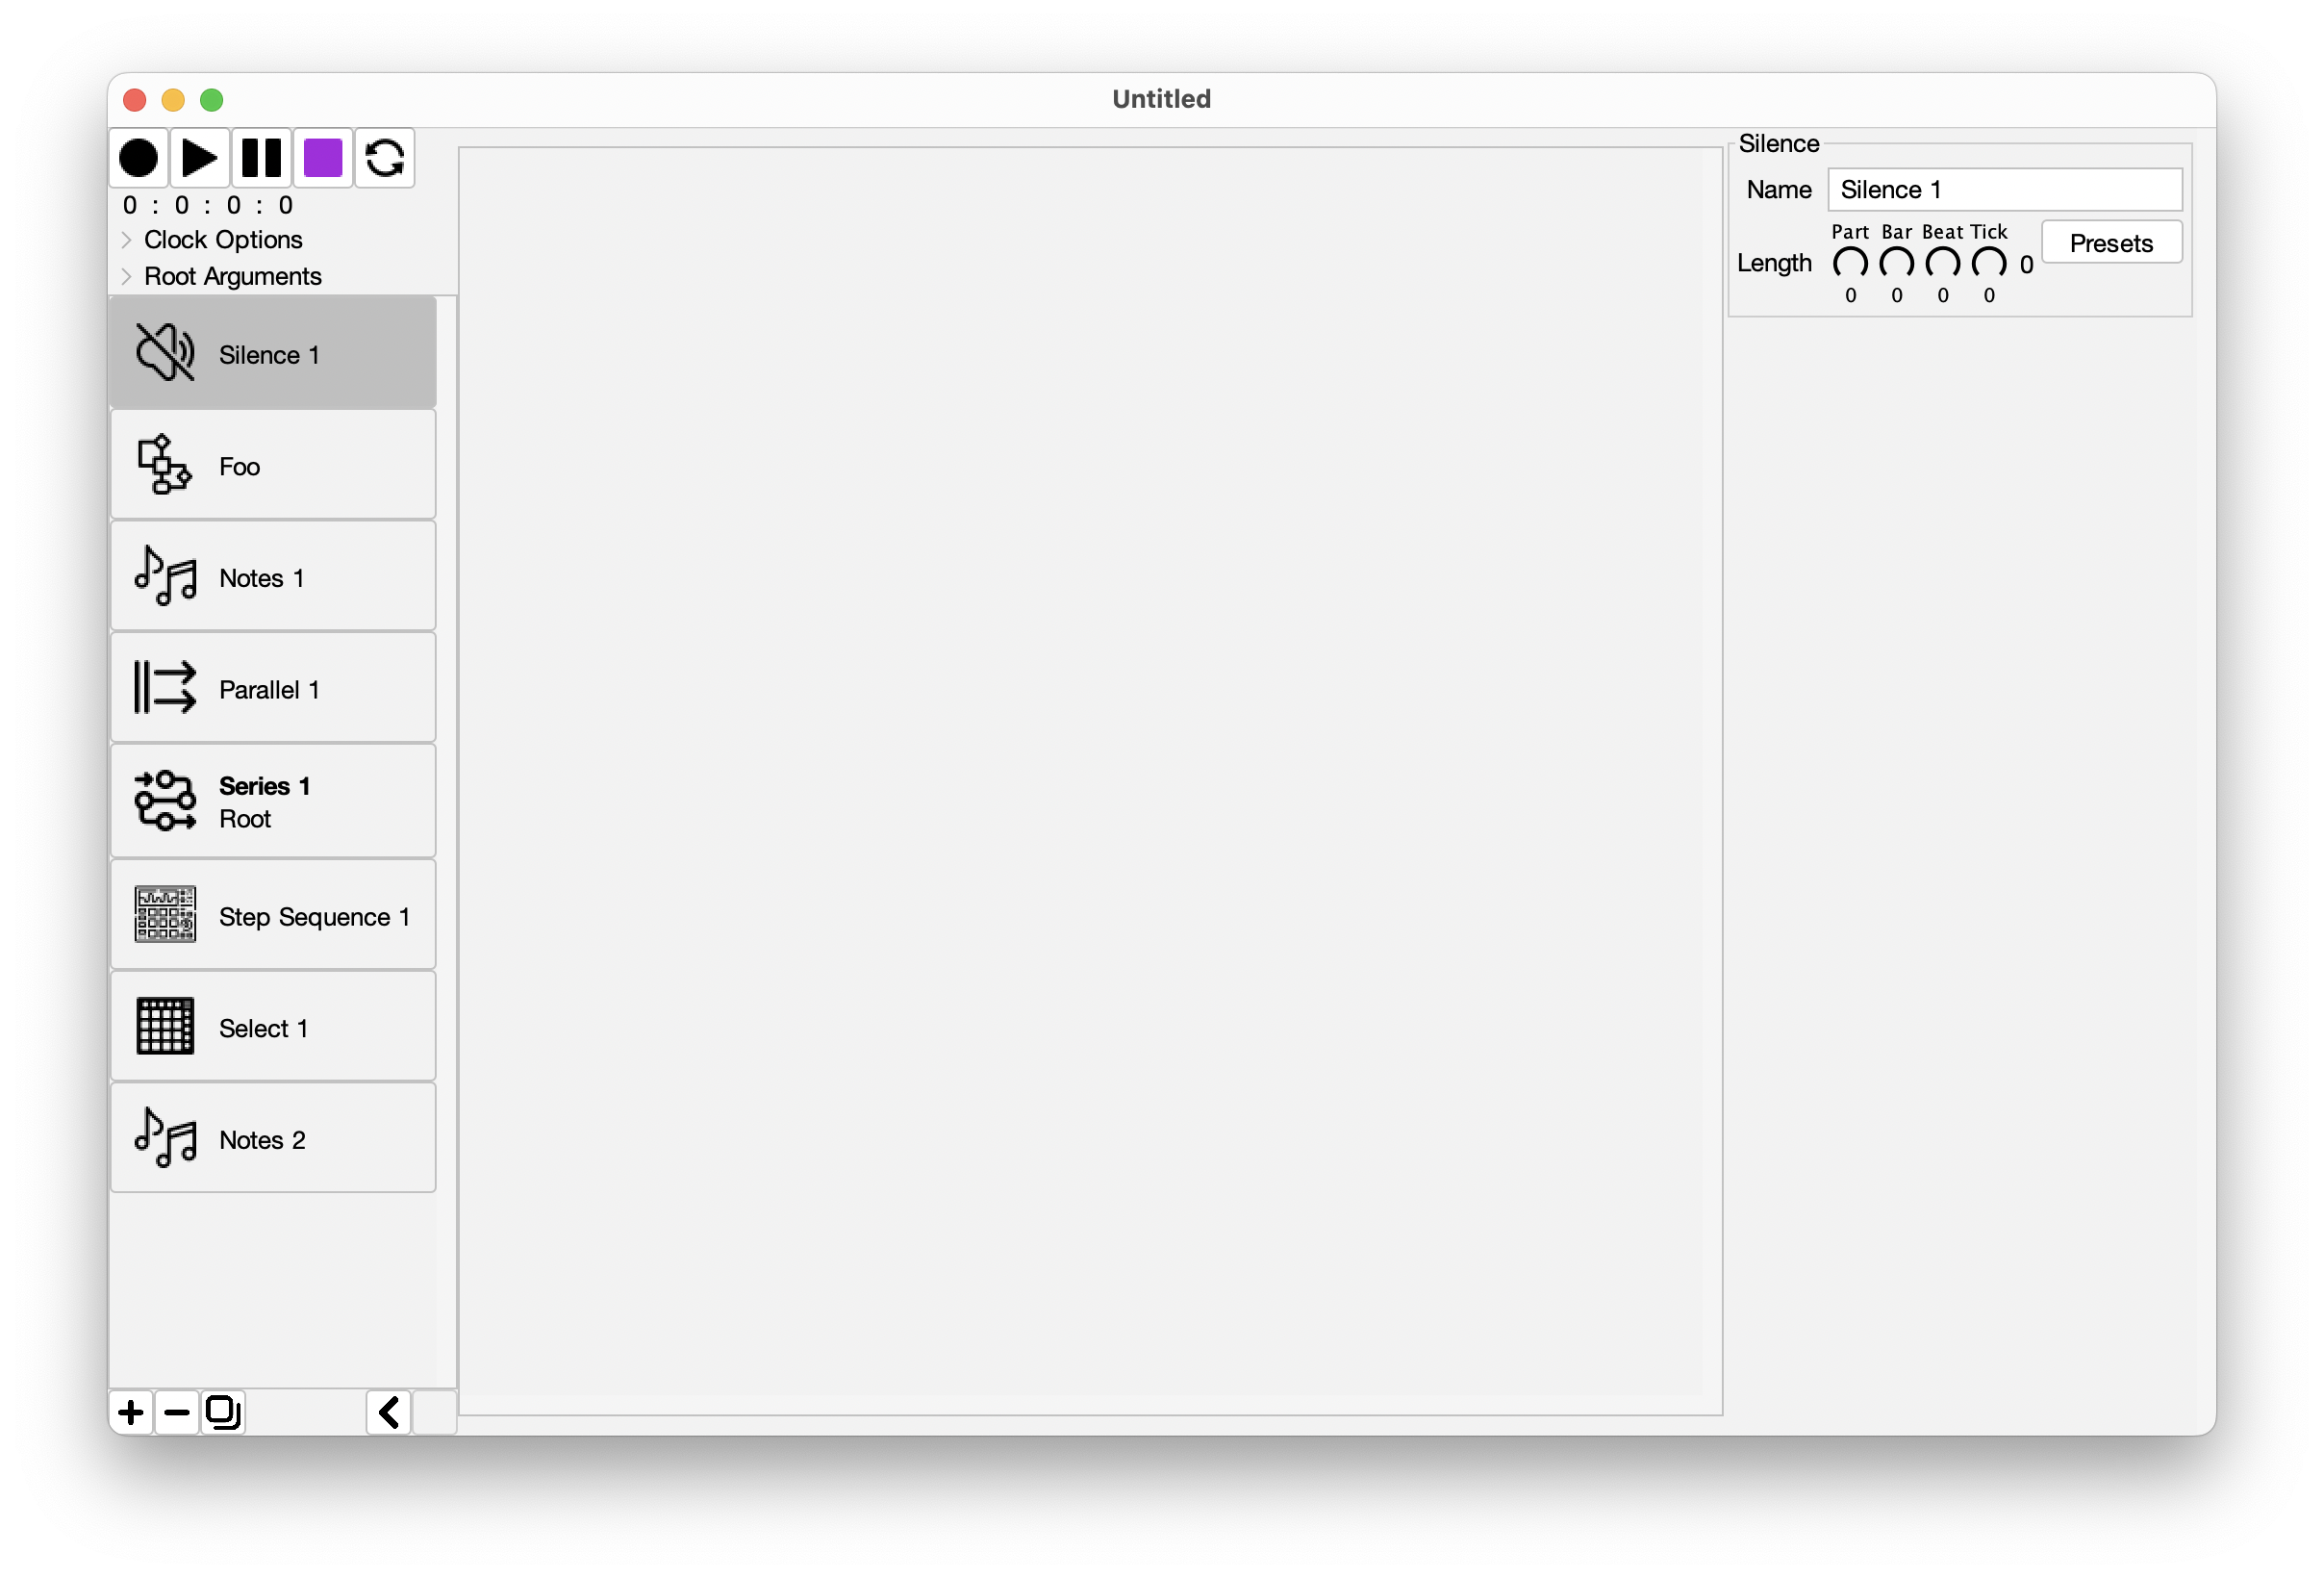
\includegraphics[width=6.5in]{Silence}
\vspace{-2em}
\caption{Silence Motif.}
\label{silence}
\end{figure}

\subsection{Silence}

Silence is nothing more than a fixed-length chunk of silence.    You can specify the {\bf length} in parts, bars (measures), beats, and ticks.  There are 192 ticks per beat, and 256 bars per part.  The number of beats per bar depends on your clock settings.

\clearpage

\begin{figure}[t]
\centering
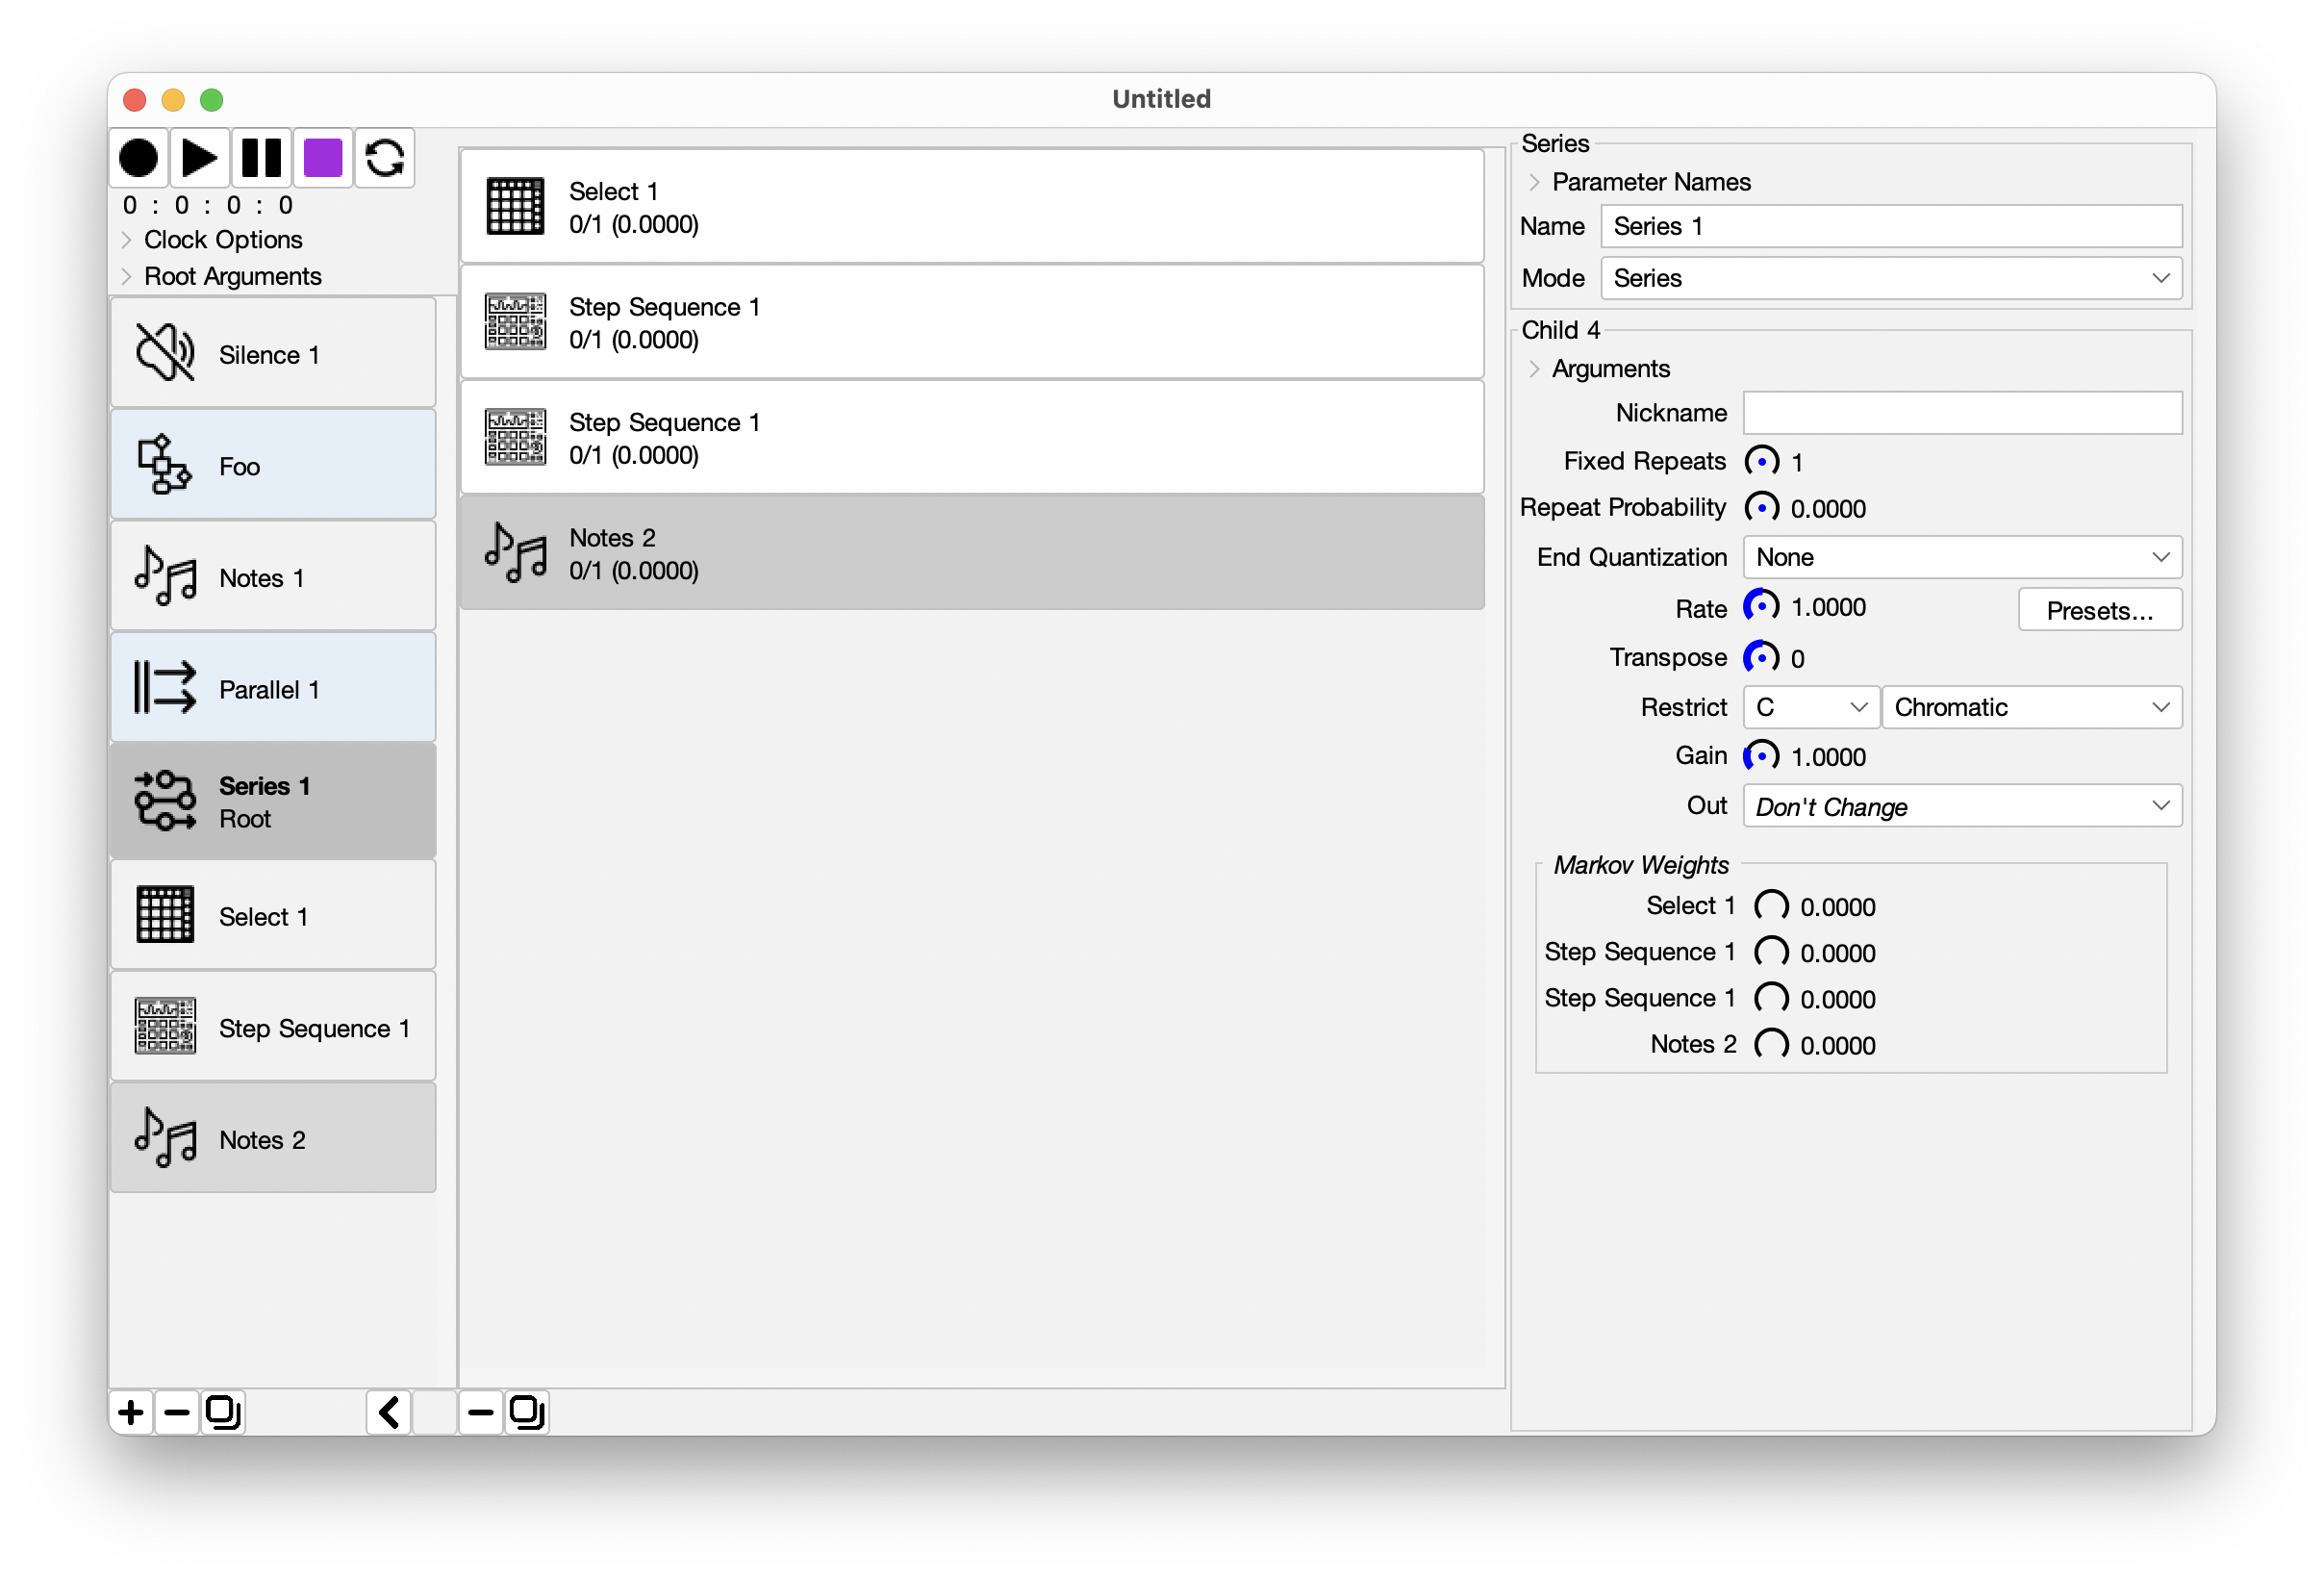
\includegraphics[width=6.5in]{Series}
\vspace{-2em}
\caption{Series Motif.}
\label{series}
\end{figure}

\subsection{Series}

By default Series is exactly what it suggests: a series of child motifs played one after another.   By ``Play'' we mean that a Child Motif is played until it is finished, and then this is repeated some \(N\) times.  That is, Series is essentially Song Mode.  

But in fact Series has several modes, and so can be set to play its children in a number of ways:

\begin{itemize}
\item{\bf Series}\quad Play each child in sequence, then finish.
\item{\bf Shuffle}\quad Randomly shuffle the order of the children.  Then play them in that order, then finish.
\item{\bf Random Forever}\quad Select a random child to play.  When finished playing it, select another one at random and play it, and so on.  Do this forever.  
\item{\bf Random Markov}\quad Select a random child to play.  When finished playing it, select a second one at random using the first child's Markov Weights, and play it.  Then select a third child at random using the second child's Markov Weights, and so on.  Do this forever.
\item{\bf Round Robin}\quad Play the first child.  When finished playing it, finish.  If you are immediately looped back to playing again, play the second child, then finish, and so on, eventually returning back to playing the first child.  Note that if you're not immediately being looped, you won't increment to the next children, but will just play the first child over and over.
\item{\bf Variation}\quad Play the child specified by Parameter 1, then finish. (For discussion of Parameters, see Section~\ref{parameters}).  This is particularly useful for creating and playing multiple {\it variations} of a given Motif.
\item{\bf Random Variation}\quad Play the child specified by the Random Parameter, then finish. (For discussion of Parameters, see Section~\ref{parameters}).
\end{itemize}

The {\bf Mode} is specified in the Series Inspector.

\paragraph{Children}

In the Current Motif Display, Series maintains a list of Child Motifs that it plays in some order or otherwise selects from.  You can drag Motifs into this list directly from the Motif List.  You can drag the same Motif to appear multiple times in the Child list.  You can also rearrange the Motifs in this list by dragging them, and can delete or duplicate a Motif in the list.

While a Child is playing, its name is highlighted in red in the Child List.

\paragraph{Child Features}
Each Child in the Child Motifs can have a {\bf Nickname}, set in its Child Inspector.  Even if a Motif appears multiple times in the List, each entry can have a different Nickname.  When you set the Nickname, it appears with the Child in the list.

When a Child finishes playing once, we can immediately go on to whatever is next to do, or we can first wait until some quantized time boundary (16th note, quarter note, or measure) before doing so.  This is set in the Inspector as {\bf End Quantization}.

When a Child is played, it is played once, and then for some number of additional iterations or {\bf Initial Repeats}.  You can set this value in the Inspector.  Thereafter, we flip a coin of {\bf Repeat Probability}, and each time it comes up heads, we play the Child once more. When it comes up tails, we stop playing the child, and go on to the next step (starting playing some other child, or finishing).  These two values are also displayed in the Child in the list, along with the number of iterations performed so far.

Alternatively if you select {\bf Until Trigger 8}, both Repeats features are ignored and the Child  will repeat forever until the Series receives a Trigger on Parameter 8.  (For discussion of Parameters, see Section~\ref{parameters}).

One Child is designated the {\bf Start}.  You choose it by selecting ``Start Here''.  If you are in {\it Series Mode}, and the Series is the {\it Root}, then when you press play, playing will begin with that Child.  If no Child is designated the Start, then the Start is 0.  The purpose of this mechanism is to temporarily allow you to change where in the song you'd like to start playing or recording.

\paragraph{MIDI Modification}

As a Child of the Series emits MIDI, that MIDI is handed to the Series, which has a chance to modify it before it is passed on.  There are several available features for modification of a given Child's MIDI in its Inspector.  {\bf Transpose} transposes all notes by some number of semitones up or down.  {\bf Restrict} forces the notes to line up with notes in a given scale: notes that don't match are transposed down to the nearest note in the scale.  {\bf Gain} changes the overall volume (velocity) of notes.  And {\bf Out} changes the MIDI Out being used (by default it is set to {\it Don't Change}.

Finally, {\bf Rate} changes the speed at which the child is played, faster or slower.  Keep in mind that Seq has a resolution of 192 ticks per beat (PPQ), so changing the speed\,---\,particularly faster\,---\,can quickly result in inaccuracies.  Some {\bf Presets} are provided, including a Custom Rate option.

\paragraph{Markov Weights}

If the Series's mode is Random Markov, the first child to play is selected entirely at random, but each subsequent child is selected using the Markov Weights of the current child.  The Markov Weights of a child are part of its features.  For a given child, each subsequent child is assigned a weight from 0.0 to 1.0 indicating the probability that it will be selected next time.  The weights are normalized to form probabilities.

For example, if you have three children, A, B, and C, and you have set A's Markov Weights to be A: 0.5, B 0.5, C 0.0, then after A has finished playing, either A or B will be selected next with equal likelihood.

\paragraph{Parameters and Arguments}

The Series Inspector has an expandable region called {\bf Parameter Names}, and each Child Inspector has an expandable region called {\bf Arguments}. Furthermore, many dials have Special Values called ``Rand'', ``Param 1'', etc.  These are explained in Section~\ref{parameters}.

The Series Inspector also has an expandable region called {\bf MIDI Parameters}.  These are discussed later in Section~\ref{mididata} (\textbf{\textit{Parameterized Control of MIDI Data}}).

\clearpage

\begin{figure}[t]
\centering
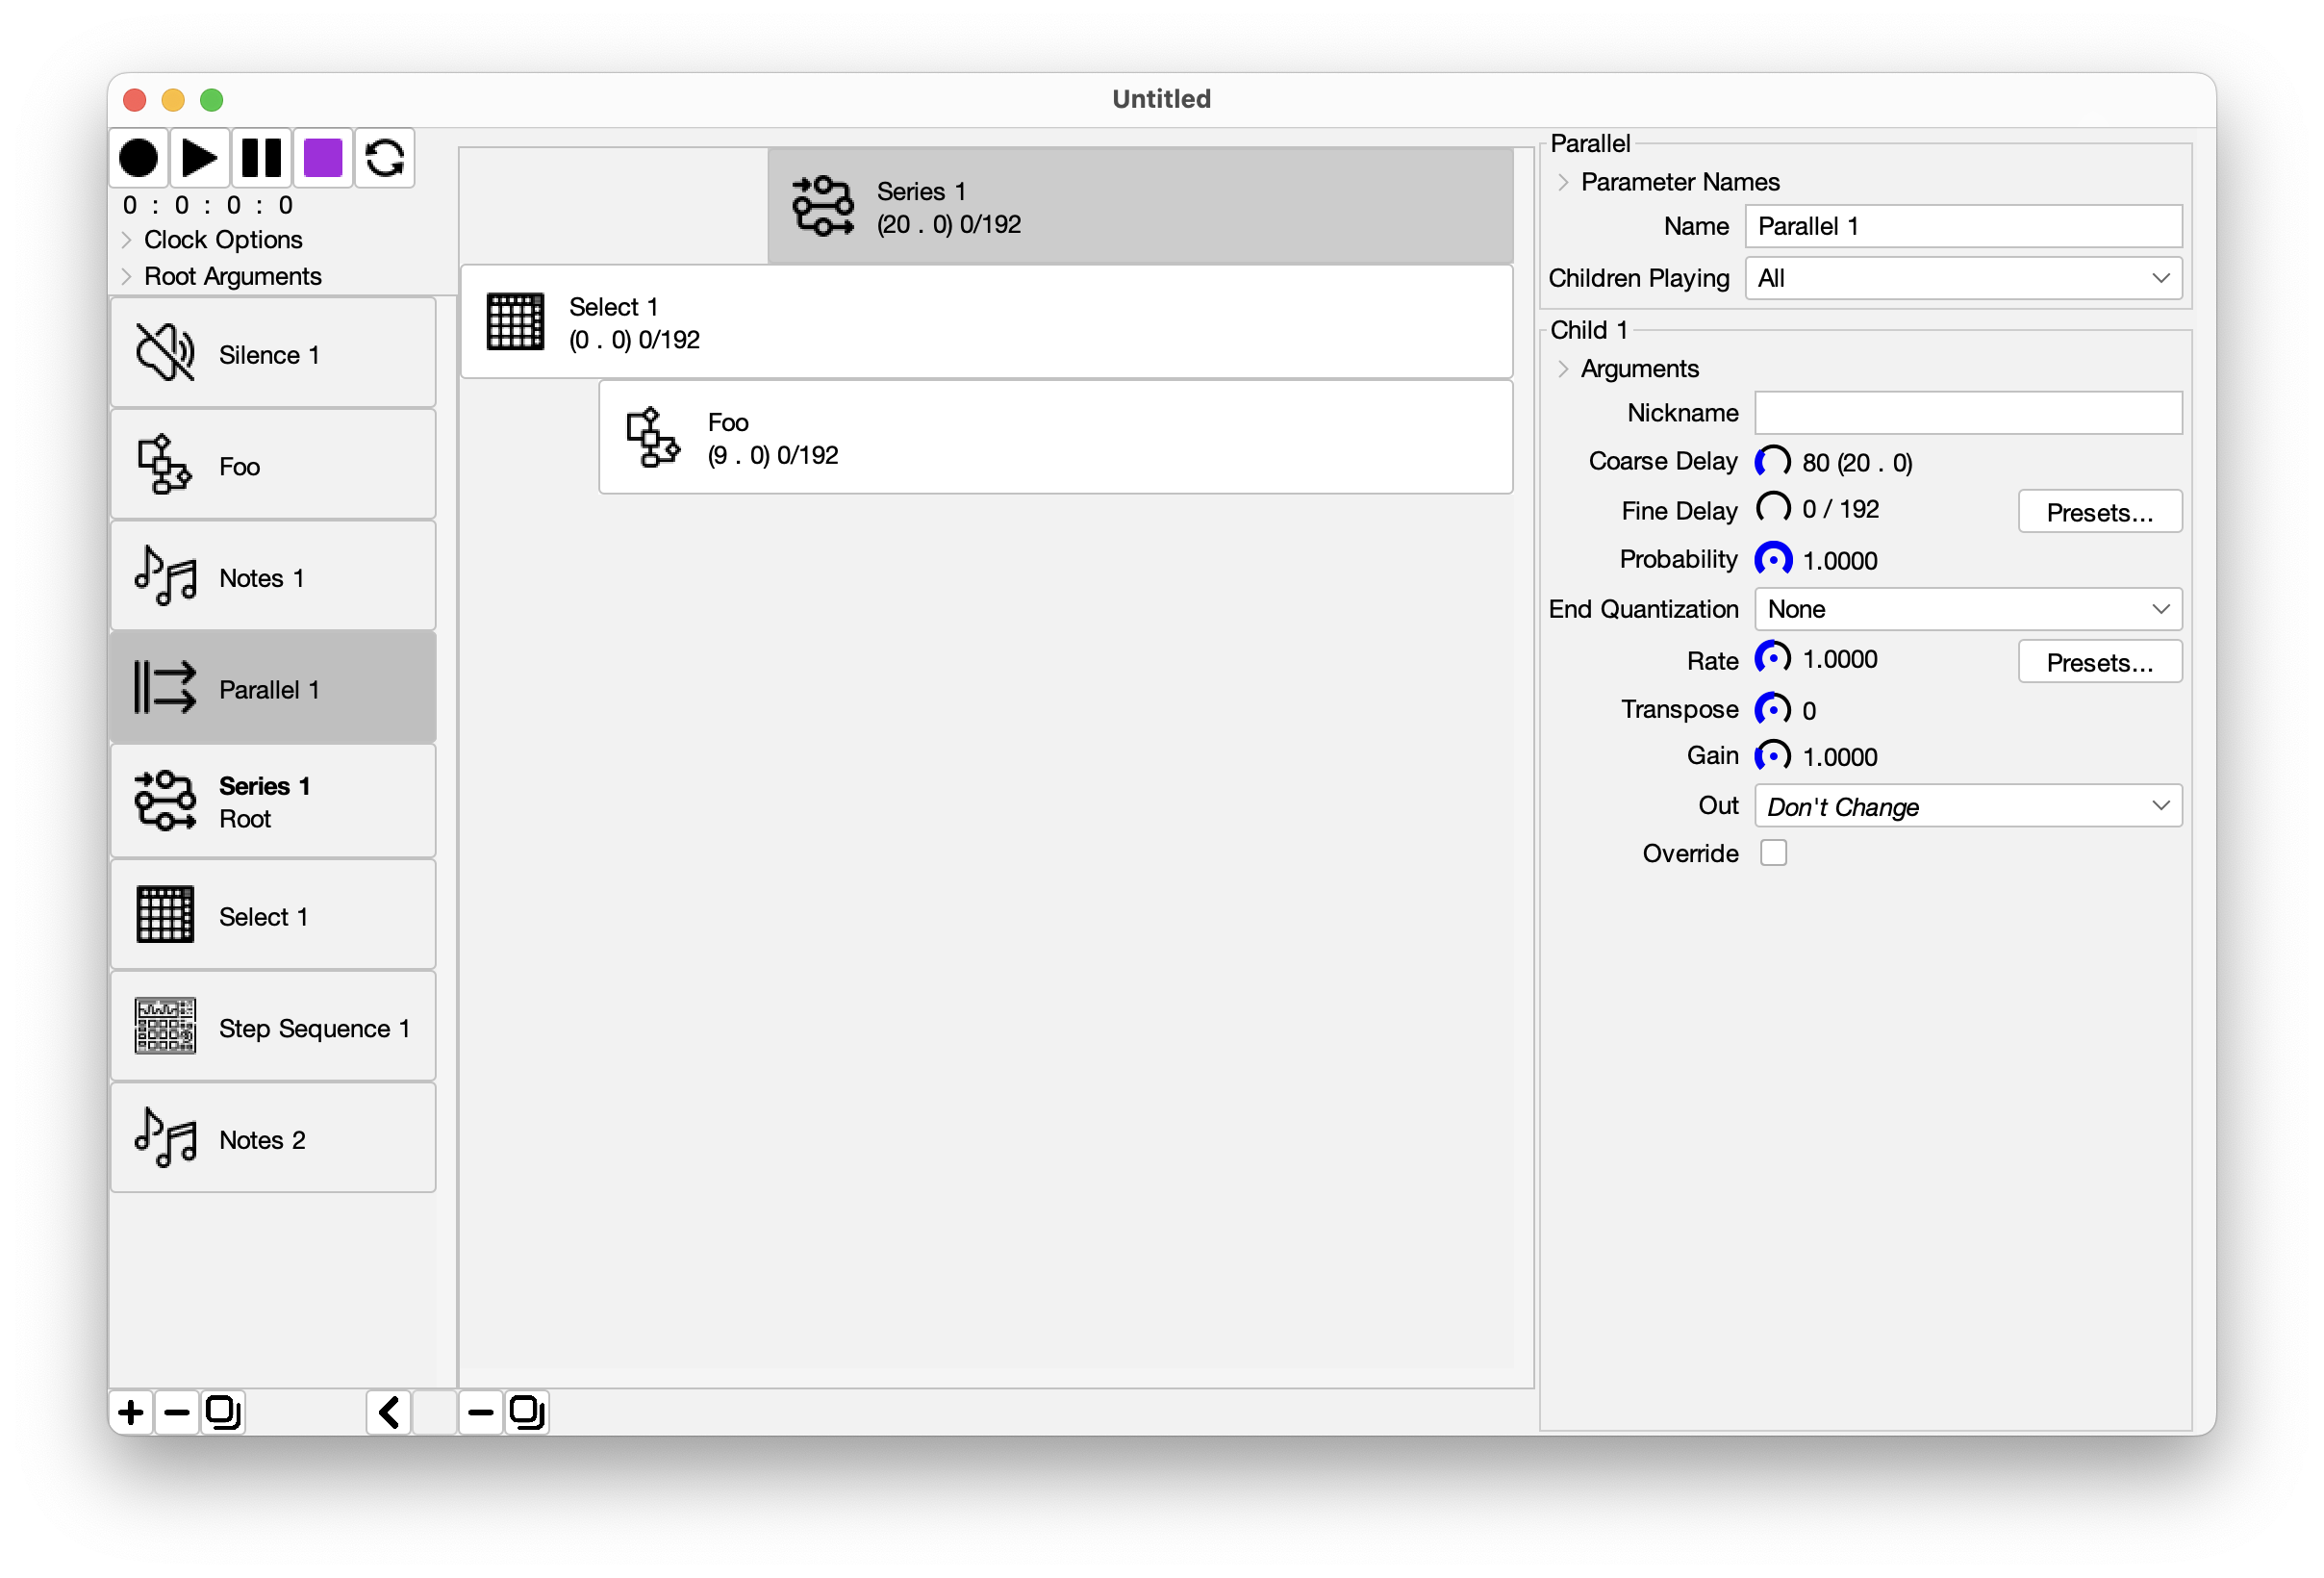
\includegraphics[width=6.5in]{Parallel}
\vspace{-2em}
\caption{Parallel Motif.}
\label{parallel}
\end{figure}

\subsection{Parallel}
\label{parallelmotif}

Like Series, Parallel is a list of of Children; but it plays them in parallel.  Each child can have its onset delayed, so that they start at different times.  Each child can have some probability as to whether it is played at all.

\paragraph{Children}

In the Current Motif Display, Parallel maintains a list of Child Motifs that it plays in some order or otherwise selects from.  You can drag Motifs into this list directly from the Motif List.  You can drag the same Motif to appear multiple times in the Child list.  You can also rearrange the Motifs in this list by dragging them, and can delete or duplicate a Motif in the list.

While a Child is playing, its name is highlighted in red in the Child List.

If a Child is playing repeated (looping) its name is highlighted in blue in the Child List.

Each Child in the Child Motifs can have a {\bf Nickname}, set in its Child Inspector.  Even if a Motif appears multiple times in the List, each entry can have a different Nickname.  When you set the Nickname, it appears with the Child in the list.

\paragraph{Cross-Fading}

Parallel can be used as a real-time cross-fader between the first two children.  The value of {\bf Cross-Fade} determines the gain of Child 1 versus Child 2.  If Cross-Fade is 0.0, then Child 1 plays at full gain and Child 2 is silenced.  If Cross-Fade is 1.0, then it's the opposite.  The default is 0.5, where each child plays at half gain.

By fault Cross-Fading is disabled, regardless of what {\bf Cross-Fade} says.  To enable cross-fading, check the {\bf Cross-Fade On} checkbox.

You can further adjust the gain of each of the children with the {\bf Gain} option in each child's inspector.  This gain is multiplied against the cross-fade gain result (if the cross-fade gain is enabled).

\paragraph{Play Probability}

Each Child has a {\bf Probability} in its Inspector.  This probability determines whether the child will be played as follows.  In the Parallel Inspector there is a feature called {\bf Children Playing}.  This feature allows you to select some \(N\) children to play when the Parallel starts playing.  Its options are:

\begin{itemize}
\item {\bf All}\quad Each child will play with its given its Probability (by default 1.0).  This is the default.
\item {\bf 1...16}\quad Parallel will select some \(N\) (1...16) children at random given their Probabilities.  These will be the only children that play.
\item {\bf All, Finish After First}\quad Every child will play with its given its Probability, except the first child in the list, which always plays.  After the first child in the list has finished playing, all children will immediately be terminated.
\end{itemize}

If a child has {\bf Override} set in its Inspector, then when it starts playing, it will immediately terminate all Children below it.  

\paragraph{Maximum End Time}

You can set the maximum end time of the Parallel with {\bf Max End Time}.  This cuts off all Children if they exceed this time.  Children (and the whole Parallel) can end sooner than the Max End Time, however.

\paragraph{Delays and Quantization}

Each Child can have the onset of its playing delayed.  Seq provides a {\bf Start} time in Parts, Bars, Beats, and Ticks, though you'll probably usually use Beats and Bars.

When the last Child finishes playing once, we can finish Parallel immediately, or we can first wait until some quantized time boundary (16th note, quarter note, or measure) before doing so.  This is set in its Inspector as {\bf End Quantization}.

When a Child is delayed, it will shift horizontally to demonstrate this, as is shown in Figure~\ref{parallel}.

\paragraph{The Ruler}
At the top of the display is the {\bf Ruler}, which shows measures and, if zoomed in, beats and sixteenth notes. 
You can zoom the Parallel in and out with the magnifying glass buttons at the bottom of the window.


\paragraph{Repeating}

After a Child has played, you can set it to {\bf Repeat}, that is, to play in a loop until all of the children have been given a chance to play at least once: basically it's vamping.  The Parallel will terminate after all Children have terminated or are looping.

While a Child is repeating, its button text color will change to blue and it will say ``REPEATING''.

{\it Why is this useful?}  Let's say you want a Step Sequence to repeat its (shorter) pattern as long as a Notes melody is playing.  That's a very common need.  There are various ways to do this, but the easiest way is to put them both in a Parallel, and set the Step Sequence to be Repeating. 

\paragraph{MIDI Modification}

As a Child of the Parallel emits MIDI, that MIDI is handed to the Parallel, which has a chance to modify it before it is passed on.  There are several available features for modification of a given Child's MIDI in its Inspector.  {\bf Transpose} transposes all notes by some number of semitones up or down.  {\bf Restrict} forces the notes to line up with notes in a given scale: notes that don't match are transposed down to the nearest note in the scale.  {\bf Gain} changes the overall volume (velocity) of notes.  And {\bf Out} changes the MIDI Out being used (by default it is set to {\it Don't Change}.

Finally, {\bf Rate} changes the speed at which the child is played, faster or slower.  Keep in mind that Seq has a resolution of 192 ticks per beat (PPQ), so changing the speed\,---\,particularly faster\,---\,can quickly result in inaccuracies.    Some {\bf Presets} are provided, including a Custom Rate option.

Unlike in other Motifs, you can {\bf Mute} children in a Parallel.  The children will still have the same length and override: they just won't produce any notes.  They will produce CC and similar data (for now).

\paragraph{Parameters and Arguments}

The Parallel Inspector has an expandable region called {\bf Parameter Names}, and each Child Inspector has an expandable region called {\bf Arguments}. Furthermore, many dials have Special Values called ``Rand'', ``Param 1'', etc.  These are explained in Section~\ref{parameters}.

One trick you can do with Probabilities: bind certain child probabilities to an argument.  Then in a parent you can mute the child at certain iterations by setting that argument to 0.0 versus 1.0.



\clearpage

\begin{figure}[t]
\centering
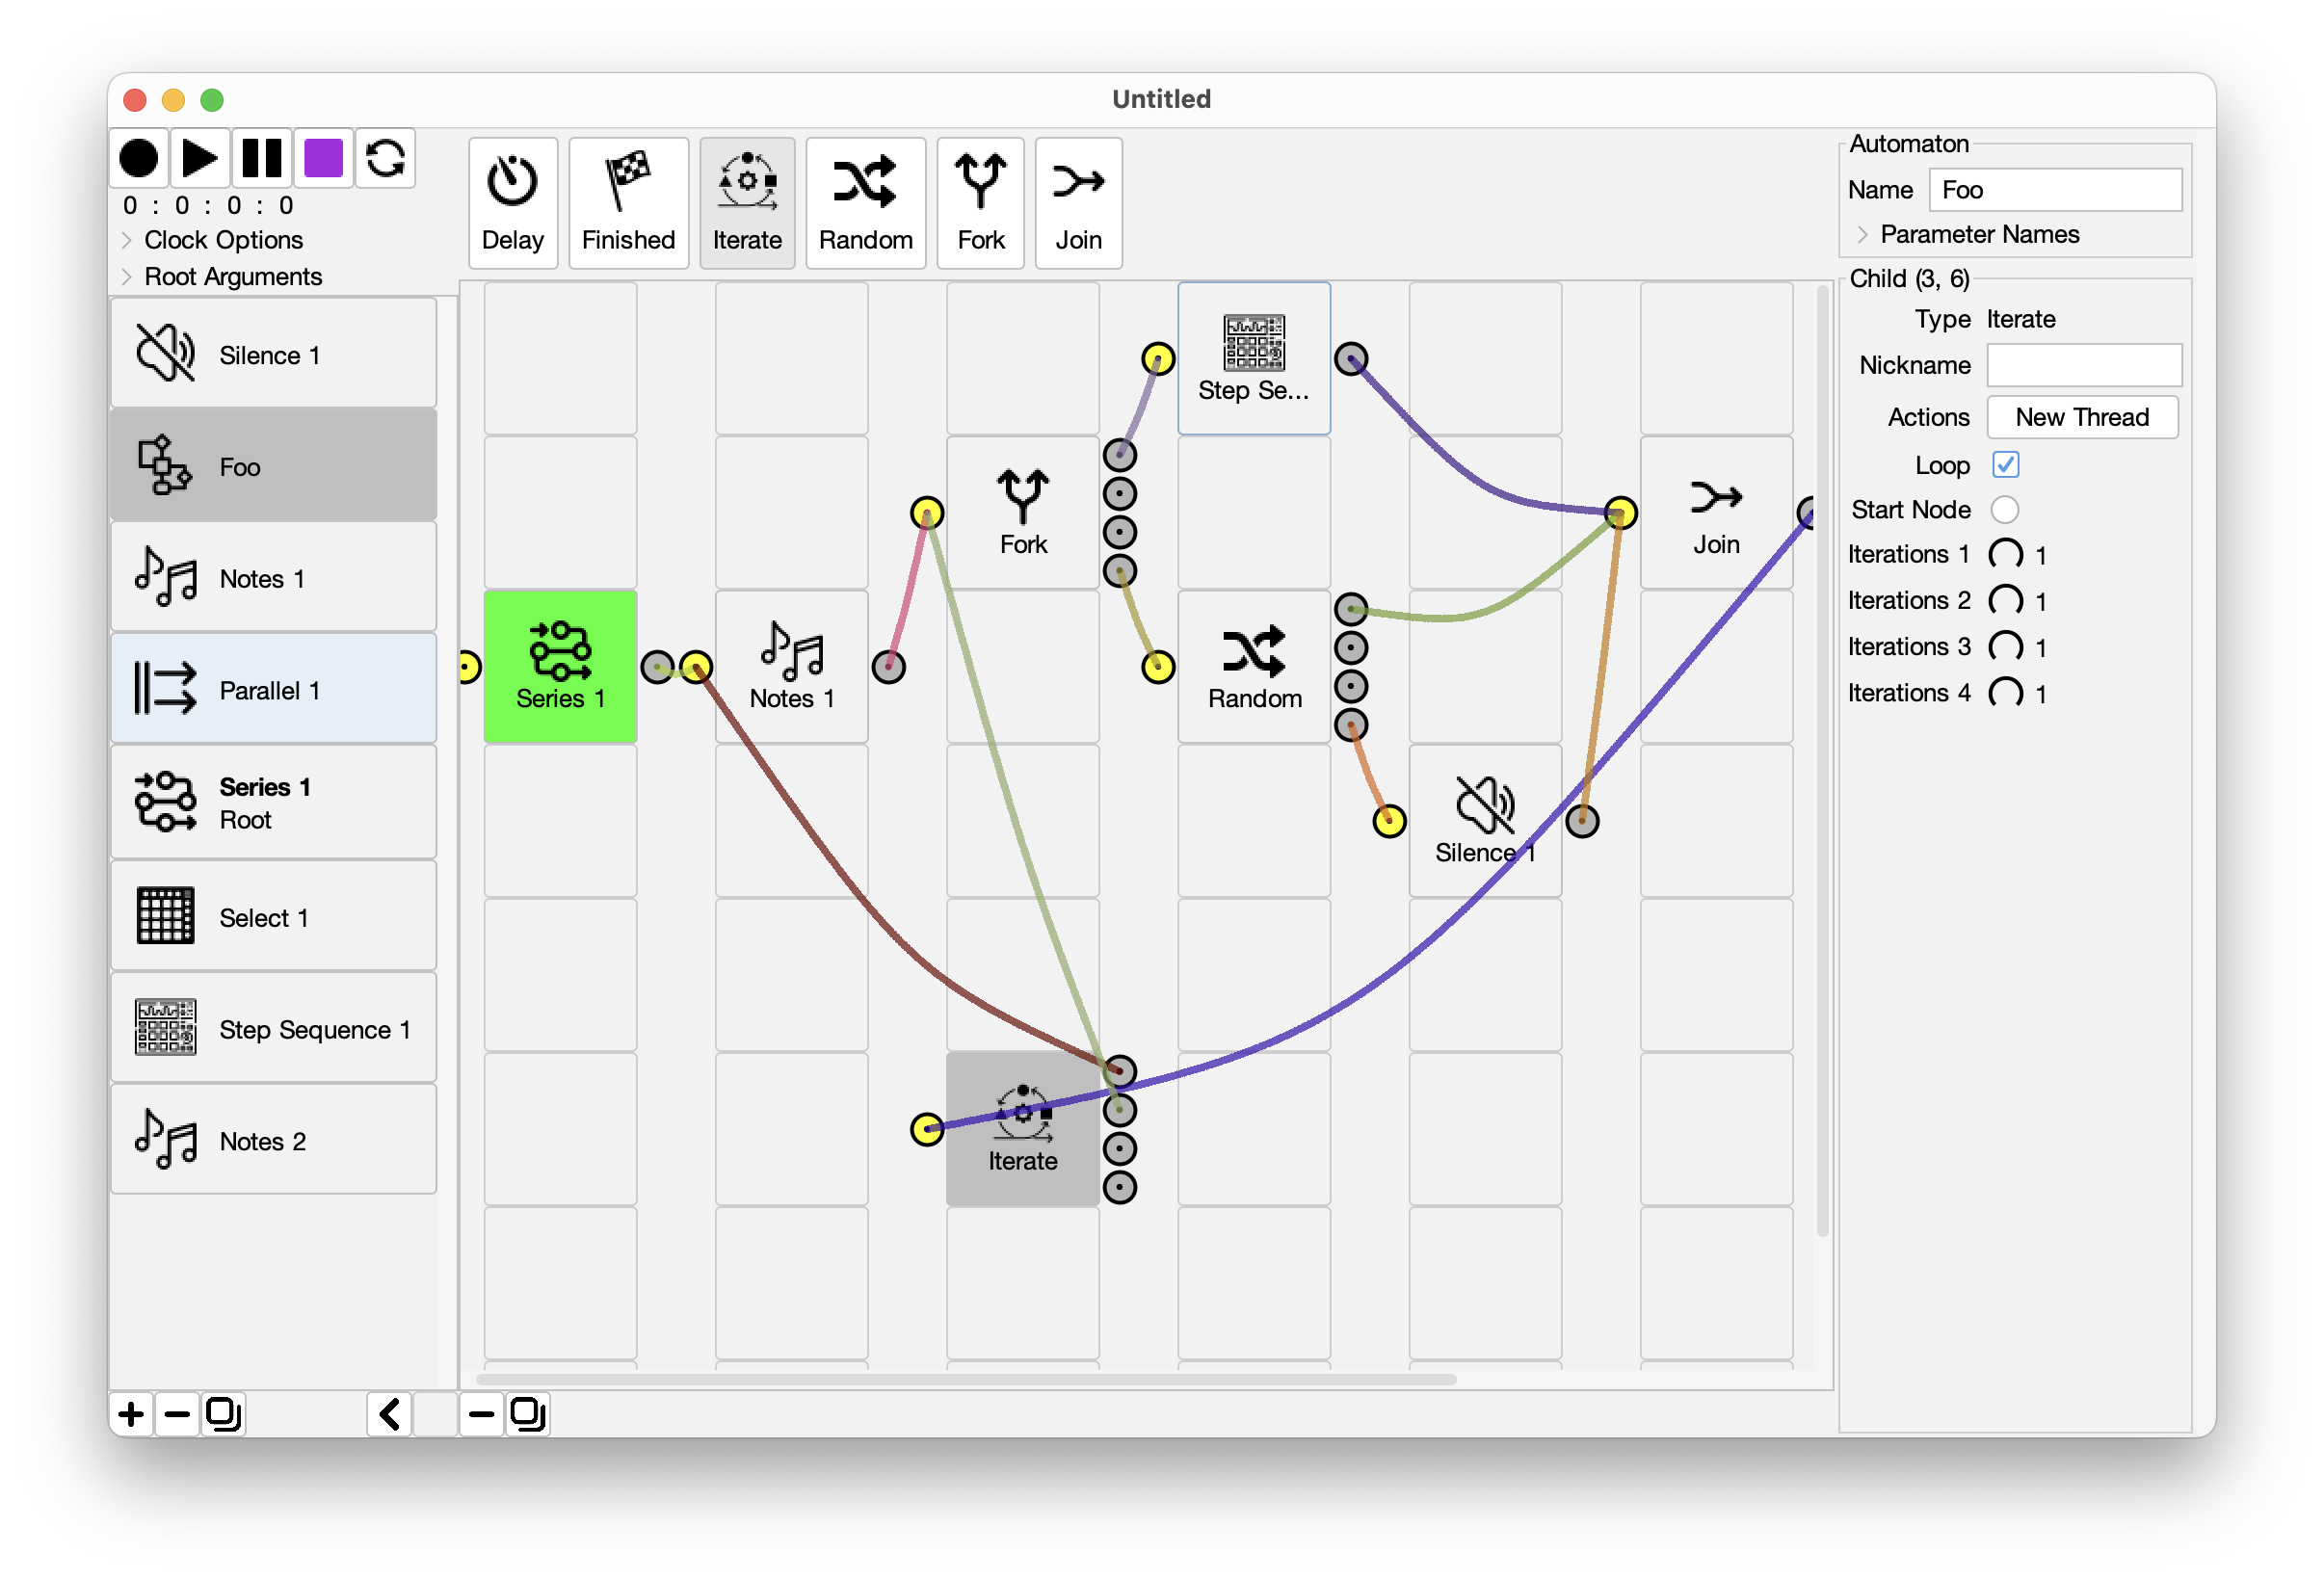
\includegraphics[width=6.5in]{Automaton}
\vspace{-2em}
\caption{Automaton Motif.}
\label{automaton}
\end{figure}

\subsection{Automaton}

Automaton may be thought of as an elaborate combination of Parallel and Select.  In Automaton you lay out Children, and various decision point nodes, then connect them to construct a diagram indicating the process you want to take place.  This is known as an {\it Automaton}.  

An Automaton contains {\bf Nodes}, that is, Children and Decision Points\,---\,and {\bf Edges}, that is, connections from Node to another.  Connections go from the endpoint of a Node to the start point of a new Node.  In our Automaton, several kinds of Nodes can have multiple endpoints, but all Nodes have just one start point.  However, while can connect many Edges to the same start point, you can connect only one Edge to a given end point.

You add Children to the Automaton by dragging them in from the Motif List.  You add Decision Points to the Automaton by dragging them in from one of the six Decision Point buttons at top ({\bf Delay, Chord, Finished, Iterate, Random, Fork,} and {\bf Join}).  You can delete a Node by selecting it, then pressing the {\bf Delete Button} at bottom, and similarly you can duplicate a Node by selecting it, then pressing the {\bf Duplicate Button}.  You can move nodes to different slots by dragging them. 

Edge are connected by dragging from an endpoint to a start point.  You can delete an edge by clicking on the endpoint from which it began.

\paragraph{Playing}

The Automaton is capable of playing multiple things at one time.  The process of playing a single item is called a {\bf Thread}.   In a Thread, a single Node is playing, and when it finished playing, it passes playing on to another Node, or if it passes to nothing, the Thread is terminated.  Threads operate independently.  There can be no more than 8 Threads playing at one time.  Normally Threads are created automatically, but you can manually start a Thread on any Node by selecting the Node and selecting {\bf Launch Thread at Node} in the {\bf Automaton} menu (if there are already 8 active threads, selecting this menu item does nothing).

One Node is designated the {\bf Start Node}.  At present it's colored ugly Lime Green.  When the Automaton is started, it initiates a single Thread, playing the Start Node.  You can designate the Start Node by selecting it and then selecting {\bf Make Start Node} in the {\bf Automaton} menu.  You can do the same thing by pressing the {\bf Start Button} (the small button labelled ``S'' at the bottom right of the Motif Display).

When a Node has finished playing, it will select one of its endpoints, and its Thread will start playing whatever is connected to that endpoint via an Edge.  If nothing is connected, then nothing new will play and the Thread will terminate.  If all Threads have terminated, then the Automaton itself will Finish: there's nothing left to play!

Some nodes take up time while playing: for example, a Notes object will take time to play its notes.  Indeed all Children must consume at least one Tick of time.  However many Decision Point Nodes take up zero time to play, and immediately transfer to other Nodes.  It's possible to set up a cycle (an infinite loop) of zero-time Decision Point Nodes, but Seq will detect this and force the to consume at least Tick of time.

\paragraph{Child Features}

Each Child has a {\bf Nickname} that you can set in its Inspector to make it easier to read.

While playing, a Child is played once, then played additional iterations, as designated by its {\bf Initial Repeats}.  Thereafter we flip a coin with a {\bf Repeat Probability} and each time it comes up heads, we play the Child again.  When it comes up tails, we stop playing the Child.

Alternatively if you select {\bf Until Trigger 8}, both Repeats features are ignored and the Child  will repeat forever until the Series receives a Trigger on Parameter 8.  (For discussion of Parameters, see Section~\ref{parameters}).

Each iteration of the Child stops (or restarts) at the nearest {\bf Quantization} after it has finished.  This can be {\it None} (no stop immediately), {\it 16th Note, Quarter Note,} or {\it Measure}.



\paragraph{The Decision Points}

Decision Points are not Children: when they are playing they do not cause other Motifs to play.  Instead, they are used to control the flow of the Automaton process.    Each Decision Point has a {\bf Nickname} that you can set in its Inspector to make it easier to read.  

There are six Decision Point Nodes at present:

\begin{itemize}
\item{\bf Delay}\quad While playing, this simply does nothing for a set period of time, then finishes.  You can set the amount of {\bf Delay} in Ticks, Beats, Bars (Measures), and Parts.  There are 192 Ticks per Beat, and 256 Bars per Part.  The number of Beats per Measure is set in the Clock Options.  There are {\bf Presets} in fractions of a Beat that you might find helpful.  Delay and Chord are the only Decision Points that takes up time.

\item{\bf Chord}\quad While playing, this plays a chord.  You can set the total {\bf length} in  You can set the {\bf Length} in Ticks, Beats, Bars (Measures), and Parts.  There are 192 Ticks per Beat, and 256 Bars per Part.  The number of Beats per Measure is set in the Clock Options.  There are {\bf Presets} in fractions of a Beat that you might find helpful.  Delay and Chord are the only Decision Points that takes up time.

You can also set the {\bf Gate Percentage}.  This is the percentage of the Length where the Chord actually plays.   You can specify both the {\bf Velocity} and the {\bf Release Velocity}, and of course up to four {\bf pitches} for the chord notes proper.

\item{\bf Finished}\quad This simply asks the Automaton to declare to its parent that it is Finished, and then terminates in zero time.

\item{\bf Iterate}\quad This Decision Point is used to perform elaborate controlled loops.  Iterate  has four endpoints.  When it starts playing, it terminates immediately in zero time and control continues out one the first four endpoints that is connected. When you start playing it {\it again}, it does the same thing.  This continues for the number of {\bf Iterations} designated for that endpoint.  When these iterations have been completed, it will start outputting at the {\it next} endpoint that is connected, and so on. 

If there are no more endpoints, and {\bf Loop} has been selected, then Iterations will loop back and start again with the first connected endpoint.  Otherwise it will terminate and not pass control any more.

Iterate normally updates its position in the loop regardless of which Thread is passing through the Iterate at the moment.  However you can change this behavior by checking {\bf Local}.   Now each Thread will have its own separate Iterate position, rather than updating a common one.  This may produce behaviors you didn't expect if you're not keeping track of which Thread is which, so you may not want to check this.

\item{\bf Random}\quad This Decision Point is used to make random decisions.  Random has four endpoints.  When it starts playing, it terminates immediately in zero time and control continues out one of its four endpoints. The endpoint selected is done so at random using the {\bf Weights} as probabilities.  If the selected endpoint is connected, the connected Node starts playing.  Otherwise, Random terminates and does not pass control. 

\item{\bf Fork}\quad This Decision Point passes control to {\it all its endpoints at the same time}, thus allowing playing of multiple Nodes in parallel.  It does this in zero time.  New Threads are created as necessary.  If Fork cannot create enough Threads (the active thread limit of 8 would be exceeded) Threads are only created up to the maximum for the earlier endpoints, and later endpoints are ignored.

\item{\bf Join}\quad This Decision Point waits until some number \(N\) of Threads have reached its start point, and then it terminates all of them, and creates a single Thread which passes control to its endpoint.  You can set \(N\) to any value from 2 to 8 (2 is the default).  Join is used to enable playing Threads to synchronize and wait for one another before terminating.  

\end{itemize}

\paragraph{MIDI Modification}

As a (Motif node) Child of the Automaton emits MIDI, that MIDI is handed to the Automaton, which has a chance to modify it before it is passed on.  There are several available features for modification of a given Child's MIDI in its Inspector.  {\bf Transpose} transposes all notes by some number of semitones up or down.  {\bf Restrict} forces the notes to line up with notes in a given scale: notes that don't match are transposed down to the nearest note in the scale.  {\bf Gain} changes the overall volume (velocity) of notes.  And {\bf Out} changes the MIDI Out being used (by default it is set to {\it Don't Change}.

Finally, {\bf Rate} changes the speed at which the child is played, faster or slower.  Keep in mind that Seq has a resolution of 192 ticks per beat (PPQ), so changing the speed\,---\,particularly faster\,---\,can quickly result in inaccuracies.    Some {\bf Presets} are provided, including a Custom Rate option.

\clearpage

\begin{figure}[t]
\centering
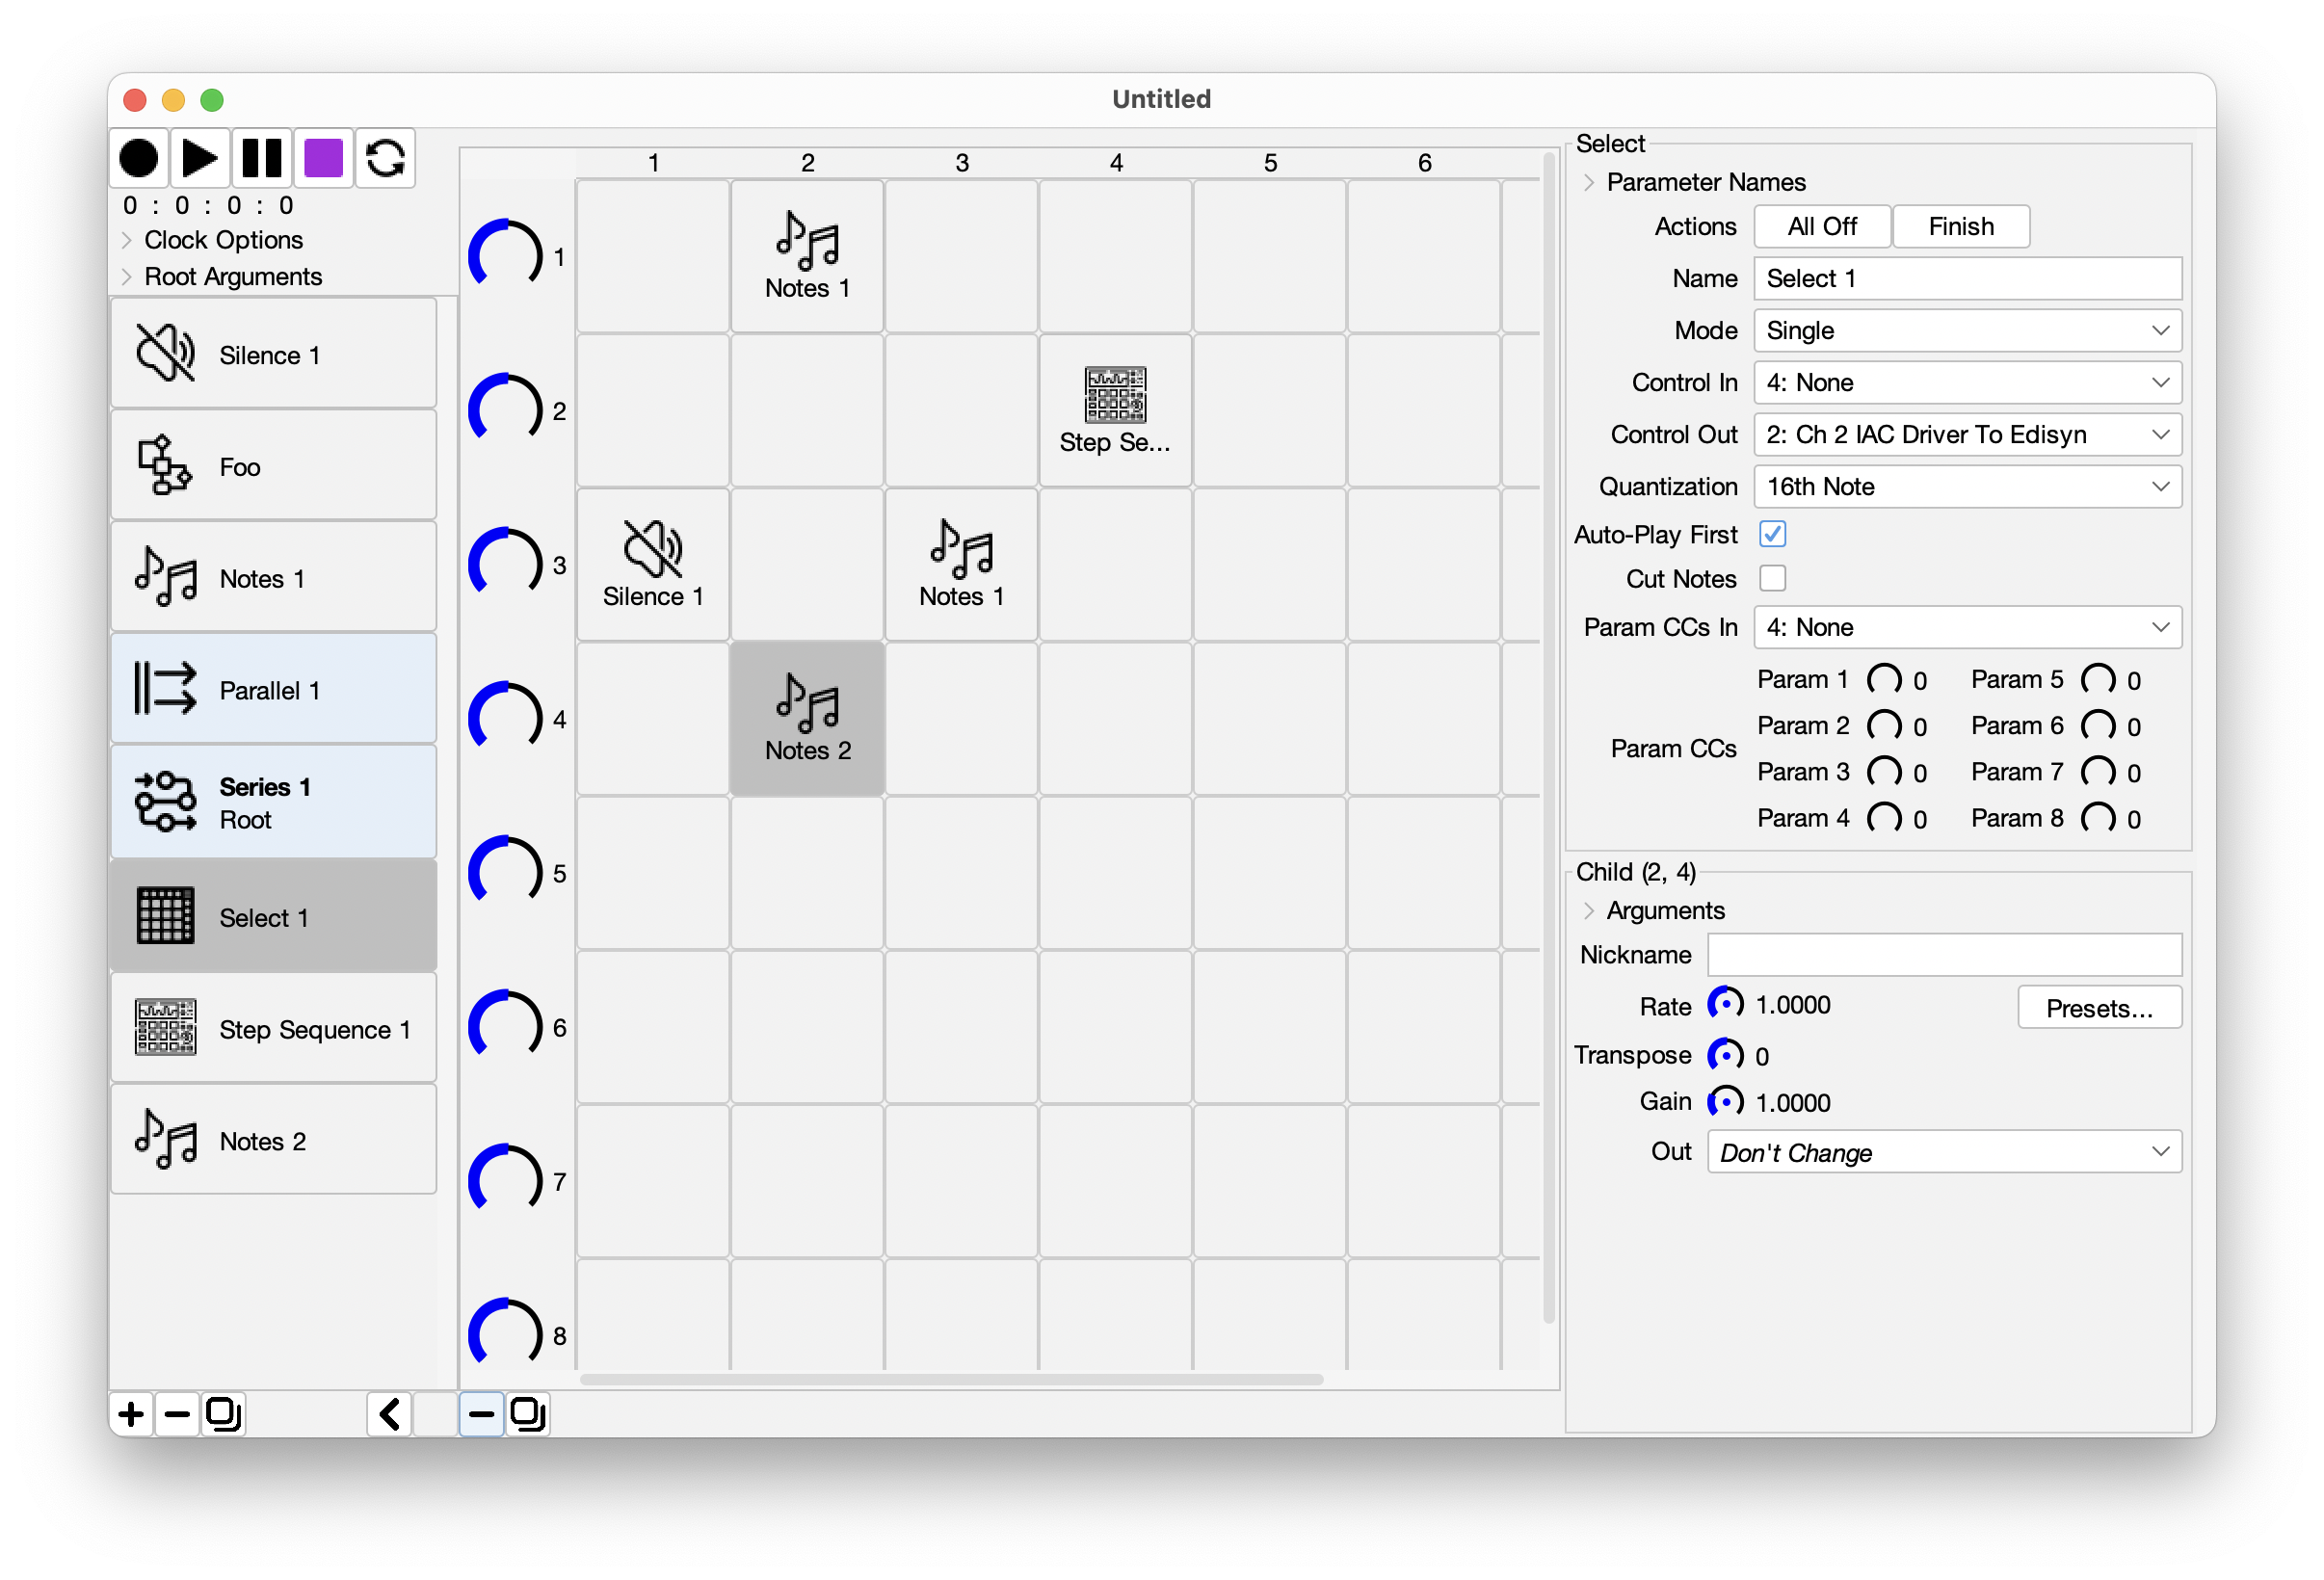
\includegraphics[width=6.5in]{Select}
\vspace{-2em}
\caption{Select Motif.}
\label{select}
\end{figure}

\subsection{Select}

Select is meant to add performance facilities to Seq.  Select is different from Series, Parallel, and Automaton: it has Children, but you as a user get to select which ones you want to play in real-time.  This can be done either via the user interface, or by connecting a Novation Launchpad MK I or MK III, or an Akai MPK Mini.  Seq also provides facilities for changing parameters, including large dials, connections to remote controllers via Control Change messages, and a large virtual joystick.

Select defines a grid where you can place Children by dragging them in from the Motif List.  The location of the Children does not matter; you can lay them out however you like.  However if {\bf Auto-Play First} is selected in the Select inspector, then the first child (most top-left) will be automatically played when Select is first played.

You can drag a Child to a new location, and you can also  delete it by selecting it and pressing the {\bf Delete Button} at bottom, and similarly you can duplicate a Child by selecting it, then pressing the {\bf Duplicate Button}. 

When you click on a Child, it is selected as usual and its Inspector will come up.  But it is not chosen to start playing.  How do you do that then?  By either middle- or right-clicking on it, or holding down any modifier key (Command, Control, Shift, Option, Alt) and clicking on it.

Each Child has a {\bf Nickname} which you can set in its Inspector.  This is useful for making a shorter name for it in the grid.



Select has four modes:

\begin{itemize}
\item{\bf Single}\quad Only one Child may play at a time, but only plays once, then terminates.  If you choose a Child to play, the old Child will stop and the new one will start.  If you select a Child which is already playing, it will play again when it has finished this time.
\item{\bf Single Repeating}\quad Only one Child may play at a time, and does so over and over.  If you choose a Child to play, the old Child will stop and the new one will start.  If you select a Child which is already playing, it will stop playing.
\item{\bf Multi}\quad Multiple Children may play at a time, but each only plays once, then terminates.  If you choose a Child to play, it starts playing.   If you select a Child which is already playing, it will play again when it has finished this time.
\item{\bf Multi Repeating}\quad Multiple Children may play at a time, and each does so over and over.  If you choose a Child to play, it starts playing.  If you select a Child which is already playing, it will stop playing.
\end{itemize}

\paragraph{Quantization and Starts and Stops}

When a new Child is selected to play, and the {\bf Quantization} is set to {\it 16th Note, Quarter Note,} or {\it Measure}, then the new Child will wait until we reach the next time Quantization before it begins playing.  In the meantime, it is colored Blue.

When a new Child is selected to play, another Child may need to stop first.   If the {\bf Quantization} is set to {\it 16th Note, Quarter Note,} or {\it Measure}, then the old Child is allowed to finish playing first (and we wait until we reach the next time Quantization).  However if {\bf Quantization} is {\it None} then the old Child is terminated immediately.

Similarly, if we have terminated a Child, Quantization determines when it will stop.

\paragraph{Other Features}

Select has an action button, {\bf Finish}.  Pressing Finish will cause Select to tell its parent that it has Finished.  This is a rare need.

%Select also can {\bf Cut Notes}.  This means that when a Child is terminated early, its notes are immediately stopped, instead of allowing the currently playing notes to finish on their own.

\paragraph{MIDI Modification}

As a Child of the Select emits MIDI, that MIDI is handed to the Select, which has a chance to modify it before it is passed on.  There are several available features for modification of a given Child's MIDI in its Inspector.  {\bf Transpose} transposes all notes by some number of semitones up or down.  {\bf Restrict} forces the notes to line up with notes in a given scale: notes that don't match are transposed down to the nearest note in the scale.  {\bf Gain} changes the overall volume (velocity) of notes.  And {\bf Out} changes the MIDI Out being used (by default it is set to {\it Don't Change}.

Finally, {\bf Rate} changes the speed at which the child is played, faster or slower.  Keep in mind that Seq has a resolution of 192 ticks per beat (PPQ), so changing the speed\,---\,particularly faster\,---\,can quickly result in inaccuracies.    Some {\bf Presets} are provided, including a Custom Rate option.


\paragraph{Parameters and Arguments}

The Select Inspector has an expandable region called {\bf Parameter Names}, and each Child Inspector has an expandable region called {\bf Arguments}. Furthermore, many dials have Special Values called ``Rand'', ``Param 1'', etc.  These are explained in Section~\ref{parameters}.

\paragraph{Overriding Parameters}
Select allows you to override parameters sent to certain children so you can control them by turning a big Dial or via a MIDI CC from a remote controller.  This is discussed later in Section~\ref{selectparameters}.

\paragraph{The Joystick}
You can assign two parameters to a Joystick available in the Inspector.  The parameters are assigned using the ``X'' and ``Y'' radio buttons in the Parameters section of the Inspector (again, see Section~\ref{selectparameters}).

\paragraph{Using a Grid Controller}

To use a Grid Controller to select Children, you specify it in the {\bf Control In} and {\bf Control Out}.  Specify the device type in {\bf Device}.  When the Select starts playing, it will reset the Launch Pad to display the same grid as your current user interface layout.  You can then choose Children by pressing buttons on the Grid Controller.

\paragraph{Available Grid Controller Devices}

\begin{itemize}
\item {\bf Novation LaunchPad MK I Series}\qquad LaunchPad, LaunchPad S, LaunchPad Pro.  Only tested on the LaunchPad S.   
\item {\bf Novation LaunchPad MK III Series}\qquad Launchpad Mini, Launchpad X, LaunchPad Pro [MK3].  Only tested on the LaunchPad Mini.  When using a MK3 device, you should use the Novation LaunchPad's {\bf MIDI IN} and {\bf MIDI OUT} devices, not its {\bf DAW IN} nor {\bf DAW OUT} ones.  
\item {\bf Akai APK Mini MK2}\qquad Mini MK2.   

\end{itemize}

\paragraph{Troubleshooting}

\paragraph{\it When I go to my Select, it plays a note on my synthesizer even when stopped.}~\\
\noindent You have the Control Out set to your synthesizer device.  Instead, set it to your Grid Controller.

\clearpage

\begin{figure}[t]
\centering
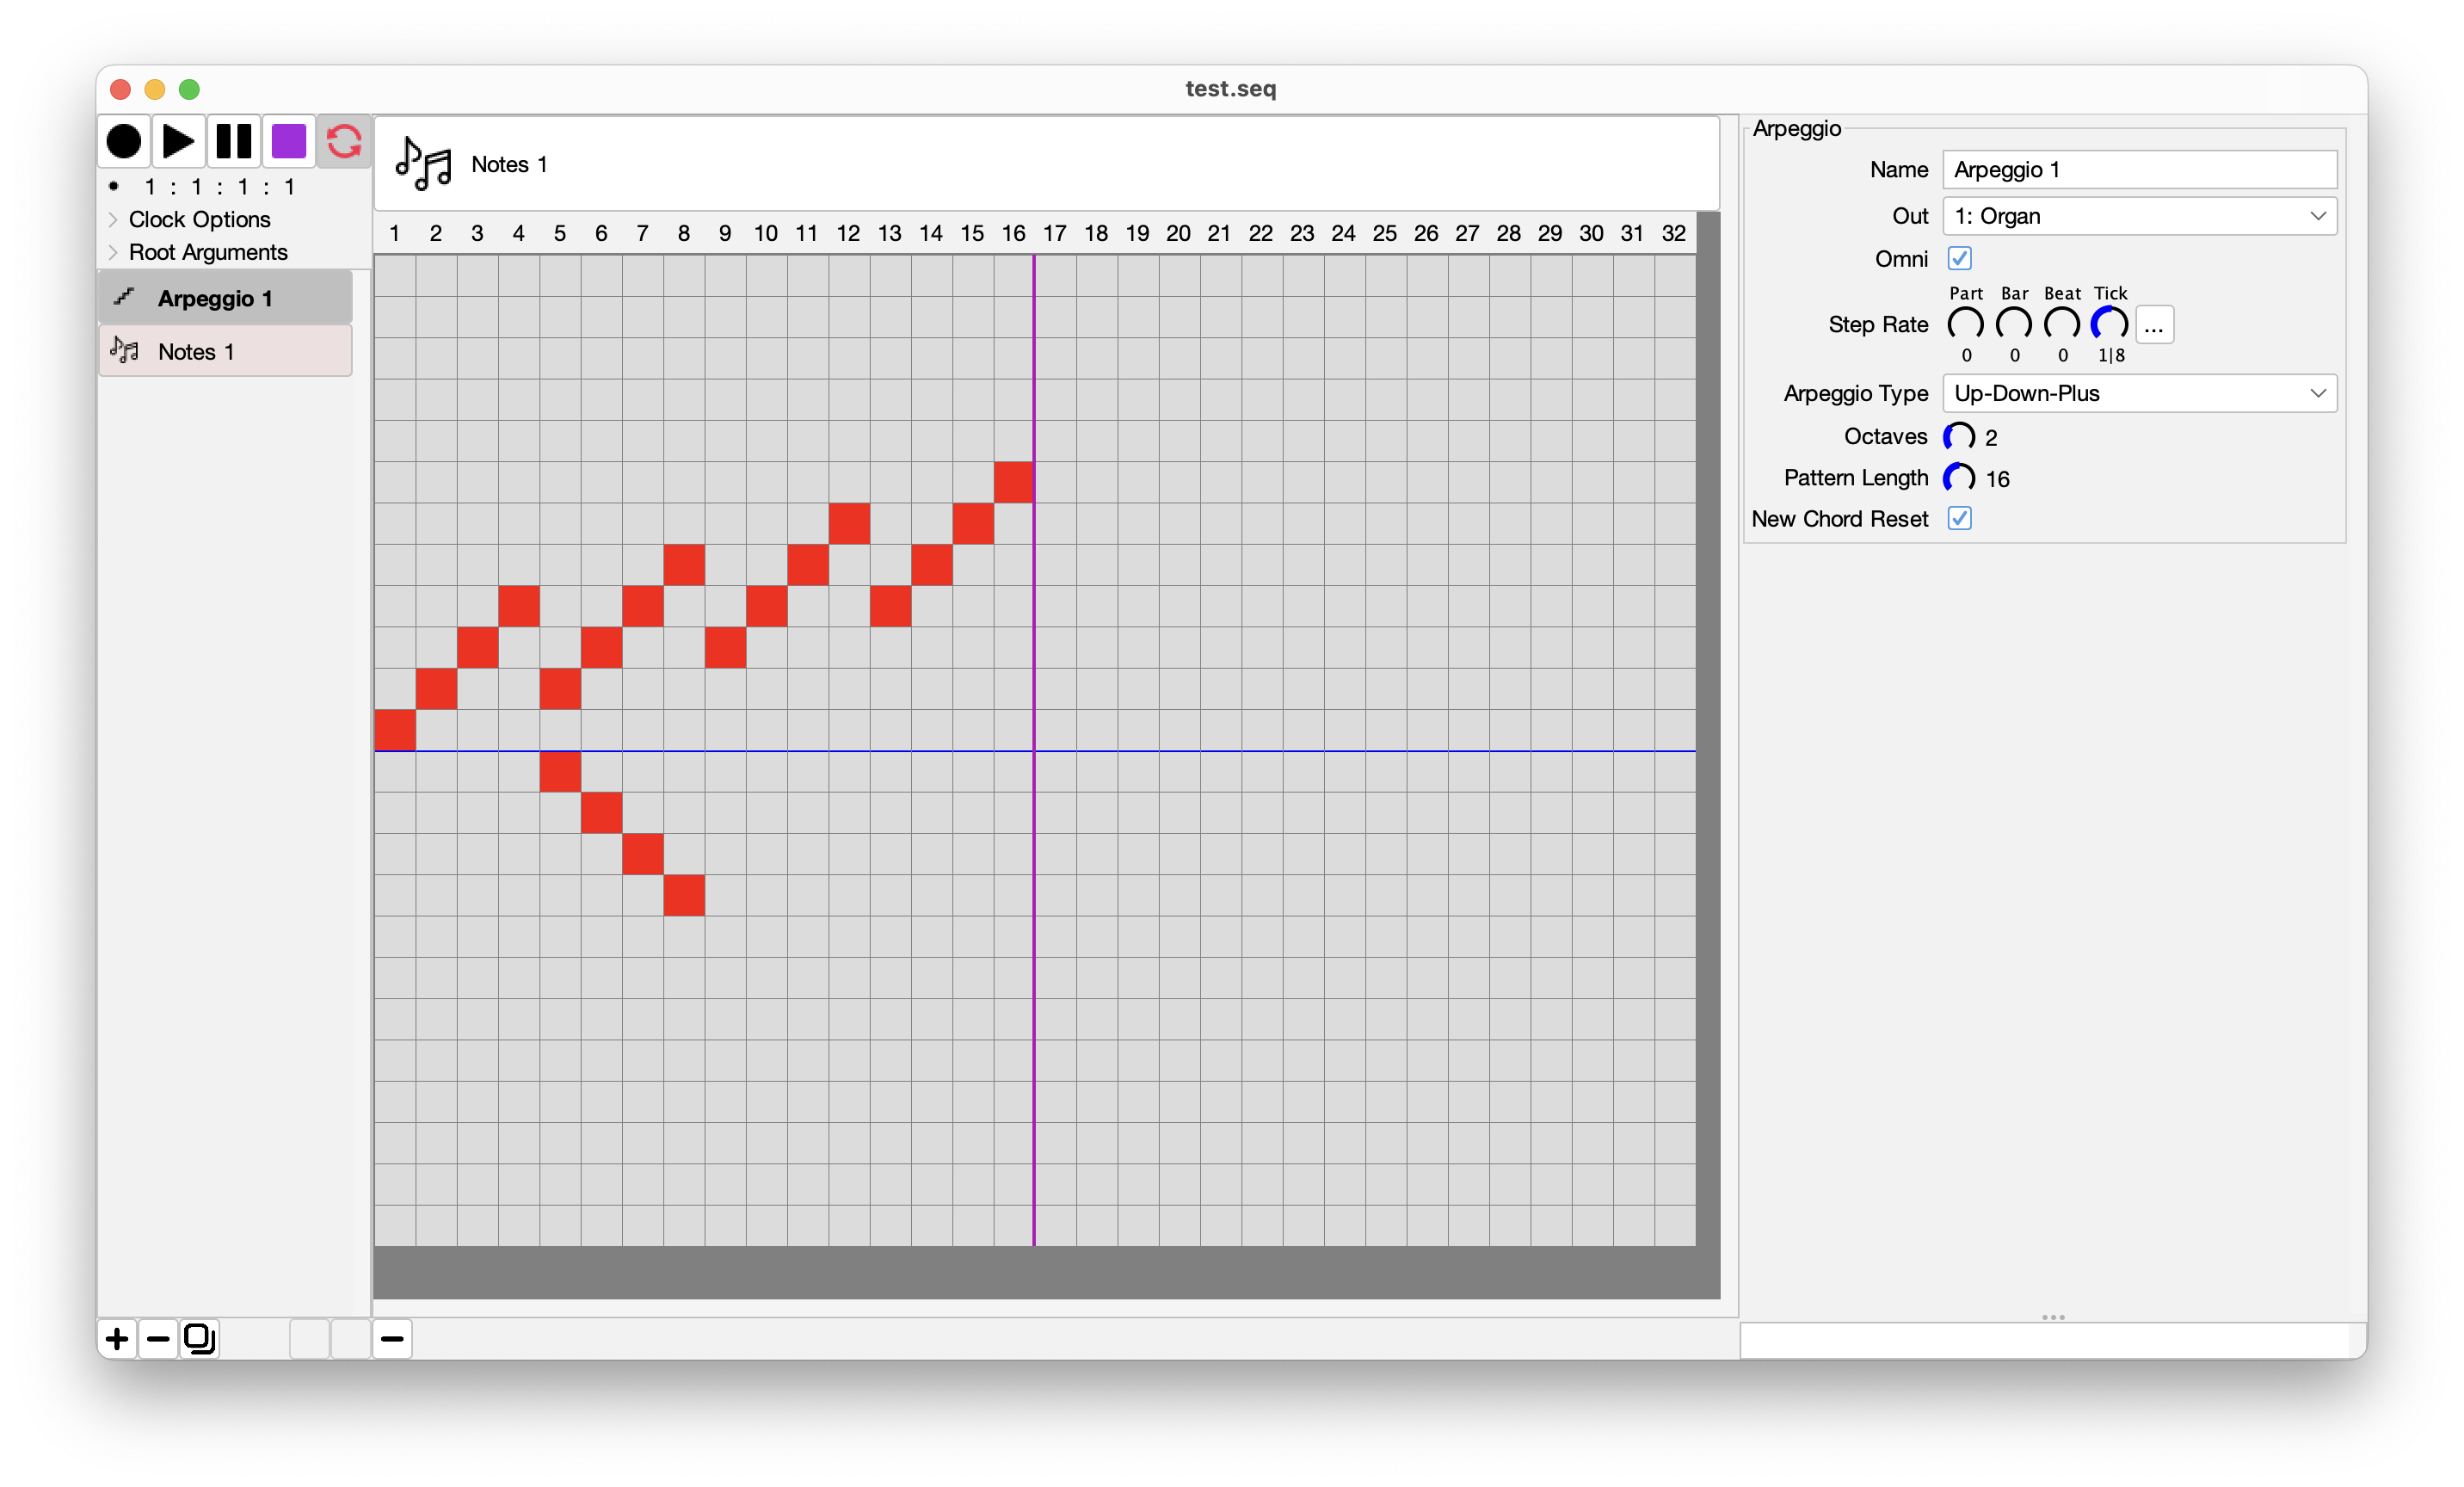
\includegraphics[width=6.5in]{Arpeggio}
\vspace{-2em}
\caption{Arpeggio Motif.}
\label{arpeggio}
\end{figure}

\subsection{Arpeggio}

Arpeggio doesn't make any sound on its own, nor does it control the order or time of play of its children.  Rather, it is a {\it MIDI Effect}: it modifies the MIDI it receives from its (only) child.  Specifically, it interprets the MIDI coming from its child as chords, and replaces them with arpeggios, just like an arpeggiator on a synthesizer.

\paragraph{Source of Chords and Emitting MIDI}

To use Arpeggio, you have to provide it with a source of chords.  Usually this will be a {\bf Notes} motif, or perhaps something that contains Notes motifs as children.  You drag your chord source from the Motif List into the single slot at the top of the Arpeggio.

When a chord source like Notes emits MIDI, it does so out some {\bf MIDI Device}.  You can instruct Arpeggio to intercept {\it all} MIDI Note data from its child, and use it to make arpeggios, by checking {\bf Omni} in the Inspector.  Otherwise Arpeggio will only intercept MIDI Note data whose device is the same as {\bf Out} (set in the Inspector).

Arpeggio itself emits MIDI in the form of arpeggios. {\bf Out} specifies the MIDI output device that it will send its arpeggios to.

\paragraph{Step Rate}

The Step Rate governs the speed of the arpeggio being played.  An arpeggio is a sequence of notes, each played in turn for the same amount of time.  The amount of time of a single not (or {\it step}) is specified by the {\bf Step Rate}.  By default this value is a 16th note.  Don't set the Step Rate to 0, which is impossible: it will instead assume you meant 1 (which is ridiculously fast).


\paragraph{Arpeggio Types}

Arpeggio can make many kinds of arpeggios, which you specify with {\bf Arpeggio Type} in its Inspector:

\begin{itemize}
\item {\bf Up} Arpeggiates the chord upwards. 
\item {\bf Down} Arpeggiates the chord downwards. 
\item {\bf Up-Down} Arpeggiates the chord upwards, then downwards but without the top note.  For example, if Arpeggio was provided the chord C E G A, it would repeat the arpeggio C, E, G, A, G, E.
\item {\bf Up-Down-Plus} Arpeggiates the chord upwards, then downwards with the root note repeated at top.  For example, if Arpeggio was provided the chord C E G A, it would repeat the arpeggio C, E, G, A, C2, A, G, E.  (Where C2 was one octave above C).  This is more useful than {\bf Up-Down} for arpeggios with multiple octaves (see below).  
\item {\bf Random} Arpeggiates the chord by playing its notes in random order.  Random attempts to not play the same note twice when reasonable. 
\item {\bf Pattern} Arpeggiates the chord according to the provided pattern.  See {\bf Patterns} below.   The {\bf Octaves} option is ignored.
\end{itemize}

An arpeggio is played for some number of {\bf Octaves}.  For example, if you set Octaves to 2, and your chord is C E G A, and you're playing an Up arpeggio, it'd repeat C E G A C2 E2 A2 G2, where C2, E2, A2, and G2 are one octave above C, E, G, and A respectively.

\paragraph{Pattern Arpeggios}

Arpeggios get fun when you start drawing patterns in the grid at the center of the window.  Each column is a step: you can have patterns up to 32 steps long, but you probably will want a shorter pattern: set the length of your pattern, in steps, with the {\bf Pattern Length} dial in the Inspector.  You'll see a purple line mark the end of the pattern.

You instruct the Arpeggio to play a note at a given step by clicking on a square to highlight it.

The blue line is the {\it Root Marker}.  The square directly above it represents the root note in whatever chord is currently provided.  The square above {\it that} represents the second note in the chord, and so on.  When you run out of notes, the next squares represent the notes in the chord repeated again, but played one octave higher.

For example, if your incoming chord was C E G A, then the first four squares in a column, above the root marker, would represent C, E, G, and A.  The next four squares would represent C1, E1, G1, and A1 (one octave above).  The next would represent C2, D2, G2, and A2, and so on

You can play notes {\it below} the chord as well!  The squares {\it below} the Root Marker represent notes one or more octaves below the chord.  For example, the first four squares below the Root Marker would be (going down) A -1, G -1, E -1, and C -1, which are all one octave below the chord.  The next four squares below them would be A -2, G -2, E -2, and C -2, and so on.

You can play more than one note in the same step: just click multiple squares.  You can also play a {\bf rest}: just have a column with no squares selected in it.  Finally, you can make {\bf ties} to extend the length of notes.   If you shift-click (or right-click) on a pattern note, you will make a tie.  A tie indicates that the immediately previous note will be lengthened and continued.  If there is no immediately previous note (it's a rest), then the tie has no effect.  Ties are blue.

\paragraph{Velocity}

By default, the velocities (volumes) of the arpeggiated notes are based on the velocities of the underlying notes provided Arpeggio.  If you uncheck {\bf As Played} in the Inspector, then you can fix the velocity of all the arpeggiated notes to a given value by setting the {\bf Velocity} dial.

\paragraph{Resetting Arpeggios}

When the underlying child says it has finished, Arpeggio will tell the same to its parent.  Arpeggios are always reset when the parent resets or loops the Arpeggio.  Also by default Arpeggios are reset when {\it all} the old notes are released and entirely new ones are played. As long as at least one note is being played, the Arpeggio won't reset.

If you want to override this chord reset behavior, so that Arpeggio doesn't reset even when all notes are released, just uncheck {\bf New Chord Reset}.

\paragraph{Activity}

Arpeggio is a filter: its main job is not to control how and when its child plays, but rather to process the MIDI received from its child.  You might wish to say {\it when} Arpeggio produces arpeggios from its child\,---\,that is,  when it is {\bf active}.  To do this, uncheck the {\bf Always} checkbox (which says that Arpeggio is always active no matter what), and set the activity time range by changing {\bf From} and {\bf To}.  

When Arpeggio is {\it inactive} it just passes its child's MIDI straight through to its parent, rather than intercepting it to do arpeggios.

\bump

\begin{figure}[t]
\centering
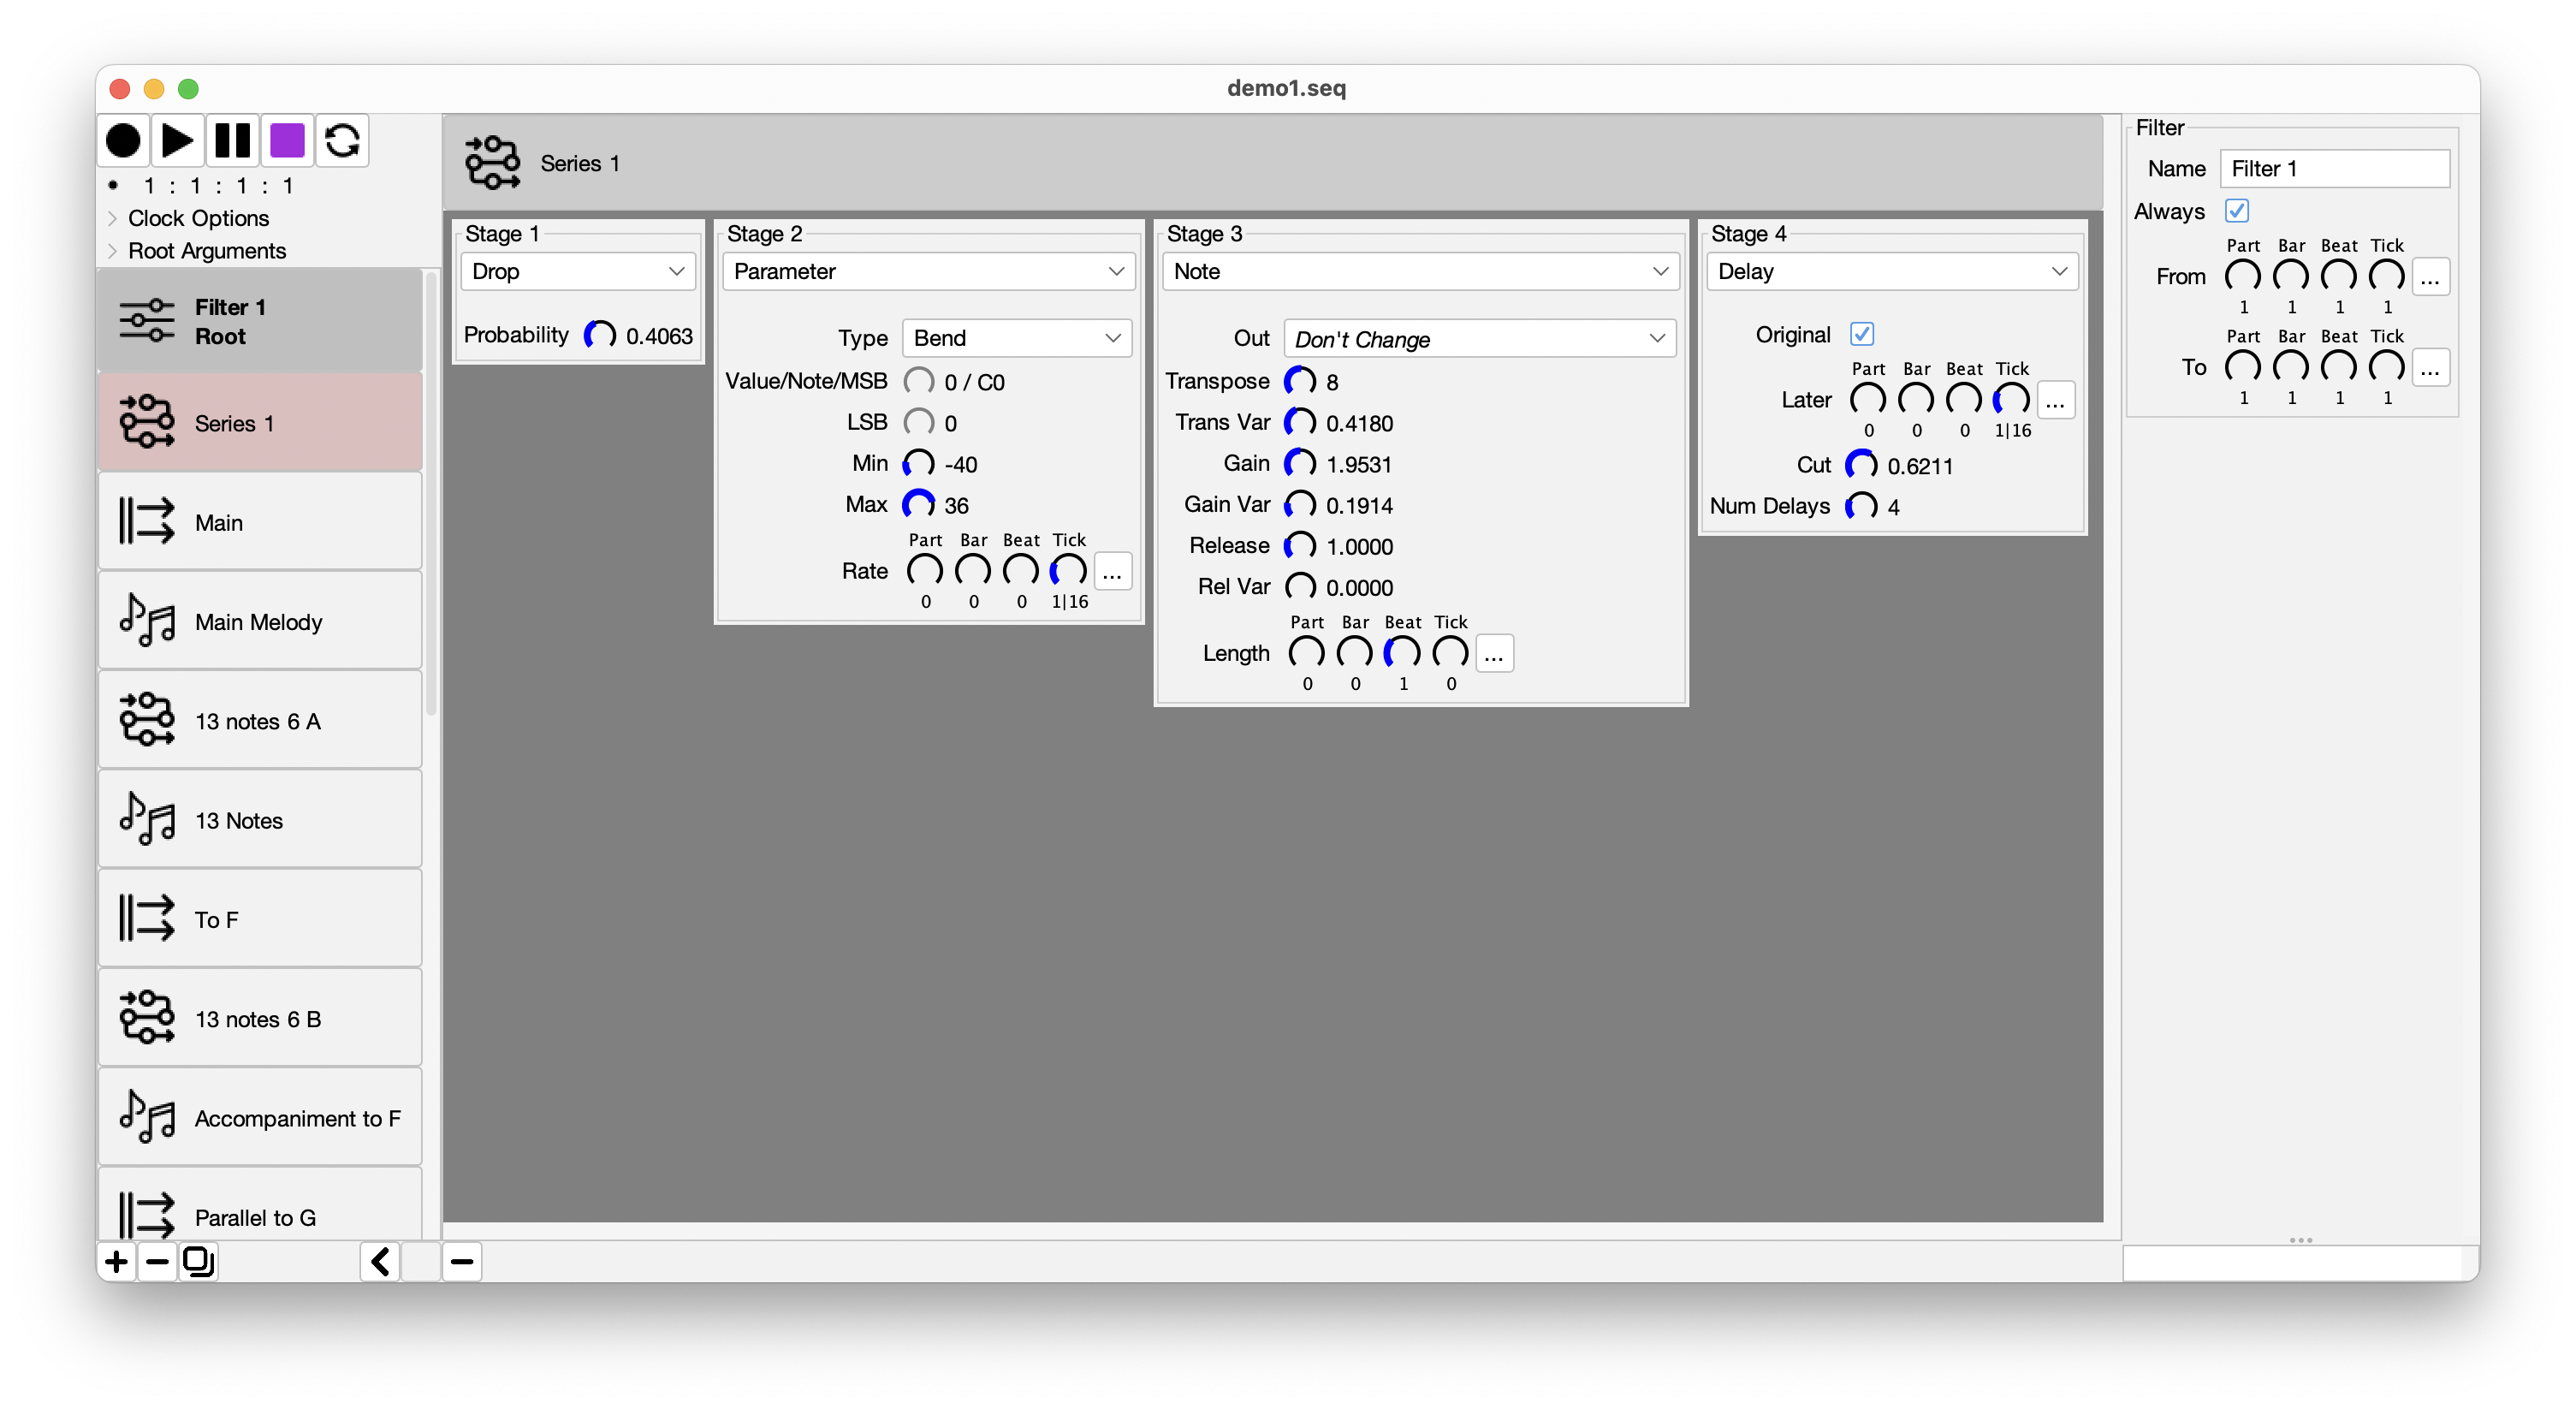
\includegraphics[width=6.5in]{Filter}
\vspace{-2em}
\caption{Filter Motif.}
\label{filter}
\end{figure}

\subsection{Filter}

Just like Arpeggio, Filter doesn't make any sound on its own, nor does it control the order or time of play of its children.  Rather, it applies a series of {\it MIDI Effects} which modify the MIDI received from Filter's (only) child.  Filter has many different ways of adding to, removing, or modifying this MIDI data.  

Filter lets you choose a MIDI Effect for each of (at present) four {\bf stages}.  When it receives MIDI data, it hands it off to the first stage, which modifies it as it sees fit.  Then it is handed to the second stage for further modification, and so on.  When all the stages have completed modification, Filter hands the resulting MIDI data to its parent, and ultimately to be emitted by Seq.

\paragraph{Activity}

Filter's MIDI Effects are only active for a certain range of time.  Outside that time, MIDI is not modified, but just passed through.   Normally this range of time is {\it all the time}, because {\bf Always} is checked in the Inspector.  If you uncheck this checkbox, you can set the activity time range by changing {\bf From} and {\bf To}.  

Filter's MIDI Effects can also be restricted to a specific Output device, which you can set with {\bf Only}.    By default they operate on {\bf All} Output devices.  Note that some MIDI Effects change the Output device of various MIDI data.  Filter decides which MIDI data will be filtered (via {\bf Only}) well before this happens, so the data will be continued to filtered regardless of what Effects change it to.

\paragraph{MIDI Effects}

At present, Filter has six MIDI Effects available:

\begin{itemize}
\item {\bf None}\qquad Doesn't change the MIDI at all.
\item {\bf Note}\qquad Changes note pitch, velocity, release velocity, and length.
\item {\bf Delay}\qquad Delays the onset of a note, or repeats it multiple times with a delay in-between, or repeats it multiple times simultaneously (as in unison).
\item {\bf Drop}\qquad With some probability, drops a note (don't let it pass through), or drops events within an interval of time.
\item {\bf Noise}\qquad Adds noise to the value of a non-note parameter such as pitch bend, CC, or aftertouch.
\item {\bf Map}\qquad Maps a non-note parameter value through a function to transform it to a different value.
\item {\bf Scale}\qquad Quantizes incoming notes, forcing them to conform to a certain scale or notes in a chord.
\item {\bf Chord}\qquad Changes an incoming note into a set of notes forming a chord or interval.
\end{itemize}

We'll describe these next in detail.  More MIDI effects are planned for the future.

At the end of this list is {\bf Copy From...}, where you can ask that a MIDI Effect in the given stage, and all of its parameters, be copied exactly from another stage.

\paragraph{The Note Effect}

This effect allows you to change features of the notes being passed in:

\begin{itemize}
\item {\bf Out}\qquad You can change the MIDI output device.
\item {\bf Non-Note Out}\qquad You change the MIDI output device for all non-note events in addition to notes.
\item {\bf Transpose and Trans Var}\qquad You can transpose all notes, and can also add random transpositions to them.  The variance ranges from \(0\) to \(\pm\) 2 octaves.
\item {\bf Gain and Gain Var}\qquad You can multiply the velocity (thus velocity) of all notes by a given gain, and can also multiply a random random gain to them.  The variance ranges from \(0\times\) to \(4\times\).
\item {\bf Release and Release Var}\qquad You can multiply the {\it release velocity} of all notes by a given gain, and can also multiply a random random gain to them.  The variance ranges from \(0\times\) to \(4\times\).
\item {\bf Change Length and Length}\qquad You can set the length of all notes.
\item {\bf Adds to Length}\qquad If checked, then you can {\it add to} the length of notes rather than {\it set} their length.  Note that {\bf Change Length} must still be checked. 
\end{itemize}

\paragraph{The Delay Effect}

This effect adds delays and unison to notes.  You can add one or more delays to an original note, and choose whether to play the original at all.  If you set the delay interval to zero, you can bulk up your original note with more of the same note, creating a {\bf unison} effect.

The Delay options are:

\begin{itemize}
\item {\bf Original}\qquad Whether to play the original note at its original time.
\item {\bf Interval}\qquad The interval between successive delays. 
\item {\bf Cut}\qquad How much to multiply the current delay volume by to get the volume of the next delay.  This eventually will cut delays down to 0 volume.
\item {\bf Num Delays}\qquad How many delays to do (besides the original, if you're playing that one).
\item {\bf Random}\qquad Whether the delay is fixed or random.  If random, then the actual delay will be between 0 and Interval in length.  This is particularly useful to humanize notes by adding a slightly randomized delay to when they're actually played.  To do this, set Original to false, set Cut to full, set Num Delays to 1, set Random to true, and then set Interval to the maximum delay length you'd want to add (usually something very small, perhaps 40 ticks).  Note that you cannot cause notes to be played slightly {\it earlier}, just {\it later}: Delay doesn't know what notes are arriving.
\end{itemize}

MIDI delays can wreak havoc on some simpleminded synthesizers.  MIDI instructs synthesizers to start playing a note with a {\it Note On} message (specifying the pitch), and to stop playing the note with a {\it Note Off} message (with the same pitch). Imagine that you have a single short delay on a long note.  The note commences with a {\it Note On}, and then the Delay issues a {\it Note On} (for the {\it same pitch}) for the delayed note.  Then the original note ends with a {\it Note Off}, followed by another {\it Note Off} for the delay.  But some synthesizers can only play {\it one note for a given pitch at a time}, so when the second {\it Note On} arrives, the first note is unceremoniously cut short to make way for the new one.  Or when the first {\it Note Off} arrives a synthesizer may not know which of the two notes to turn off; or it may turn off both notes, and so on.    Finally, a large delay count may overwhelm the total number of notes a synthesizer can play at one time, causing it to take drastic measures to compensate.

If your notes are short enough, and have a long enough time between them, such that delays never overlap with a note of the same pitch, then you'll probably be fine.  Otherwise, expect Delay to present challenges to your synthesizer.


\paragraph{The Drop Effect}

This effect randomly deletes notes, and also deletes all notes and non-note events within a certain region.

\begin{itemize}
\item {\bf Delete All}\qquad Whether we should delete all notes and non-note events.
\item {\bf Note Probability}\qquad If {\bf Cut} is unchecked, then the probability that a note should be deleted at random.
\end{itemize}

\paragraph{The Noise Effect}

This effect adds noise to the values of non-note parameters.  Every so often this effect chooses a new random value, then consistently adds that value to all the parameters that arrive of the given type.

\begin{itemize}
\item {\bf Type}\qquad The parameter type in question to add noise to.  The options are {\it Pitch Bend}, {\it Control Change} (CC), {\it Non-Registered Parameter Numbers} (NRPN), {\it Registered Parameter Numbers} (RPN), and {\it Aftertouch}.
\item {\bf Param/MSB}\qquad The parameter to add noise to.  Pitch Bend doesn't have a parameter.  Aftertouch also doesn't have a parameter (note is disregarded\,---\,all aftertouch messages are treated the same).
  For NRPN and RPN, this serves as the {\it Most Significant Byte} (MSB) of the parameter to add noise to.
\item {\bf LSB}\qquad The {\it Least Significant Byte} of the parameter to add noise to.  This is only used by NRPN and RPN, and complements the MSB.
\item {\bf Variance}\qquad The noise variance, from 0.0 to 1.0.  The highest noise variance adds extreme noise to the parameter.
\item {\bf Rate}\qquad How often the parameter noise value is updated.
\end{itemize}

\paragraph{The Map Effect}

This effect maps the values of a non-note parameter to different parameters.  It does this as follows:\footnote{Note that if the parameter is pitch bend, and the value is negative, it is first made positive before any of this; then the result is made negative again at the end.}

\begin{enumerate}
\item It takes the value and bounds it between a min and a max.
\item It maps the range min...max to 0...1, so the value is now between 0 and 1.
\item It pushes the value through a function, for example, squaring the value.  The input and output are always between 0 and 1.
\item It then maps from 0...1 back to min...max, so the value is now back in its normal range.
\item It emits the final mapped value.
\end{enumerate}

This allows you to change parameter values in many ways. You could invert them, add an amount to them, square them or invert-square them (kind of like a square root), etc.

\begin{itemize}
\item {\bf Type}\qquad The parameter type in question to add noise to.  The options are {\it Pitch Bend}, {\it Control Change} (CC), {\it Non-Registered Parameter Numbers} (NRPN), {\it Registered Parameter Numbers} (RPN), and {\it Aftertouch}.
\item {\bf Param/MSB}\qquad The parameter to add noise to.  Pitch Bend doesn't have a parameter.  Aftertouch also doesn't have a parameter (note is disregarded\,---\,all aftertouch messages are treated the same).
  For NRPN and RPN, this serves as the {\it Most Significant Byte} (MSB) of the parameter to add noise to.
\item {\bf LSB}\qquad The {\it Least Significant Byte} of the parameter to add noise to.  This is only used by NRPN and RPN, and complements the MSB.
\item {\bf Map}\qquad The mapping function used.  See below.
\item {\bf Min}\qquad The minimum of the bounding range.
\item {\bf Max}\qquad The maximum of the bounding range.
\item {\bf By}\qquad A value used by some mapping functions to determine how strong their effect is.
\end{itemize}

\newcommand\param{{\text{\it param}}}
\newcommand\by{{\text{\it by}}}

The mapping functions are as follows.  Let \(\param\) be the parameter and \(\by\) be the value of the {\bf By} dial.  Both of these values range from 0 to 1.  The result of the mapping function is bounded to be within 0 and 1.

\begin{itemize}
\item {\bf None}\qquad \(\param\) is not modified at all.
\item \(\param \leftarrow \by - \param\).  This is particularly useful if \(\by = 1\): this just inverts \(\param\), making high values low and vice versa.
\item \(\param \leftarrow \param + \by\).
\item  \(\param \leftarrow \param - \by\).
\item \(\param \leftarrow \param \times \by\).  This sounds like it makes \(\param\) bigger but in fact it makes it smaller, since \(\by \leq 1\).
\item Discretize \(\param\) by \(by\).  This creates a stairstep effect.  Here, \(\by\) is treated as a value from 1 to 16.   \(\param\) is set to the nearest division of 1.0 into \(\by\) chunks.  For example, if \(\by = 8\). and \(\param\) is 0.352, then \param is rounded up to 0.375 (that is, \(3/8\)).  
\item Discretize \(\param\) by \(by\), and subtract from 1 (inverting it).
\item \(\param^2\).  This makes \(\param\) rise more slowly and in a curved fashion.
\item \(\param^4\).  This makes \(\param\) rise even more slowly and in a curved fashion.
\item \(1-(1-\param)^2\).  This makes \(\param\) rise faster and in a curved fashion.
\item \(1-(1-\param)^2\).  This makes \(\param\) rise even faster and in a curved fashion: it's much like the exponential rise in an envelope.
\end{itemize}

\paragraph{The Scale Effect}

This effect forces incoming notes to quantize to the nearest note in a scale or chord.

\begin{itemize}
\item {\bf Key}\qquad The key of the scale or chord.
\item {\bf Round}\qquad How to force the incoming notes. You can {\bf round down} the note to the nearest note in the scale/chord equal to or below the incoming note.  Or you can {\bf round up} to the nearest note equal to or above the incoming note.  Or you can round the incoming note to the {\bf nearest} note in the scale/chord: if you do this, ties are broken by rounding {\bf up} or {\bf down}.
\item {\bf The Notes}\qquad You can select which notes in the scale or chord you want to force the note to conform to.  A variety of {\bf Presets} are also offered.
\end{itemize}

\paragraph{The Chord Effect}

This effect converts a note into a full chord or interval.  It is similar to the classic {\it chord memory} effect in certain synthesizers.

\begin{itemize}
\item {\bf Chord/Interval}\qquad The chord or interval to convert the note to.
\end{itemize}



\paragraph{Parameterization}

Many Effect features can be {\bf Parameterized} by double-clicking on the dials.  For more on parameterization, see Section~\ref{parameters}, (\textbf{\textit{Parameterized Control of MIDI Data}}).



\clearpage

\begin{figure}[t]
\centering
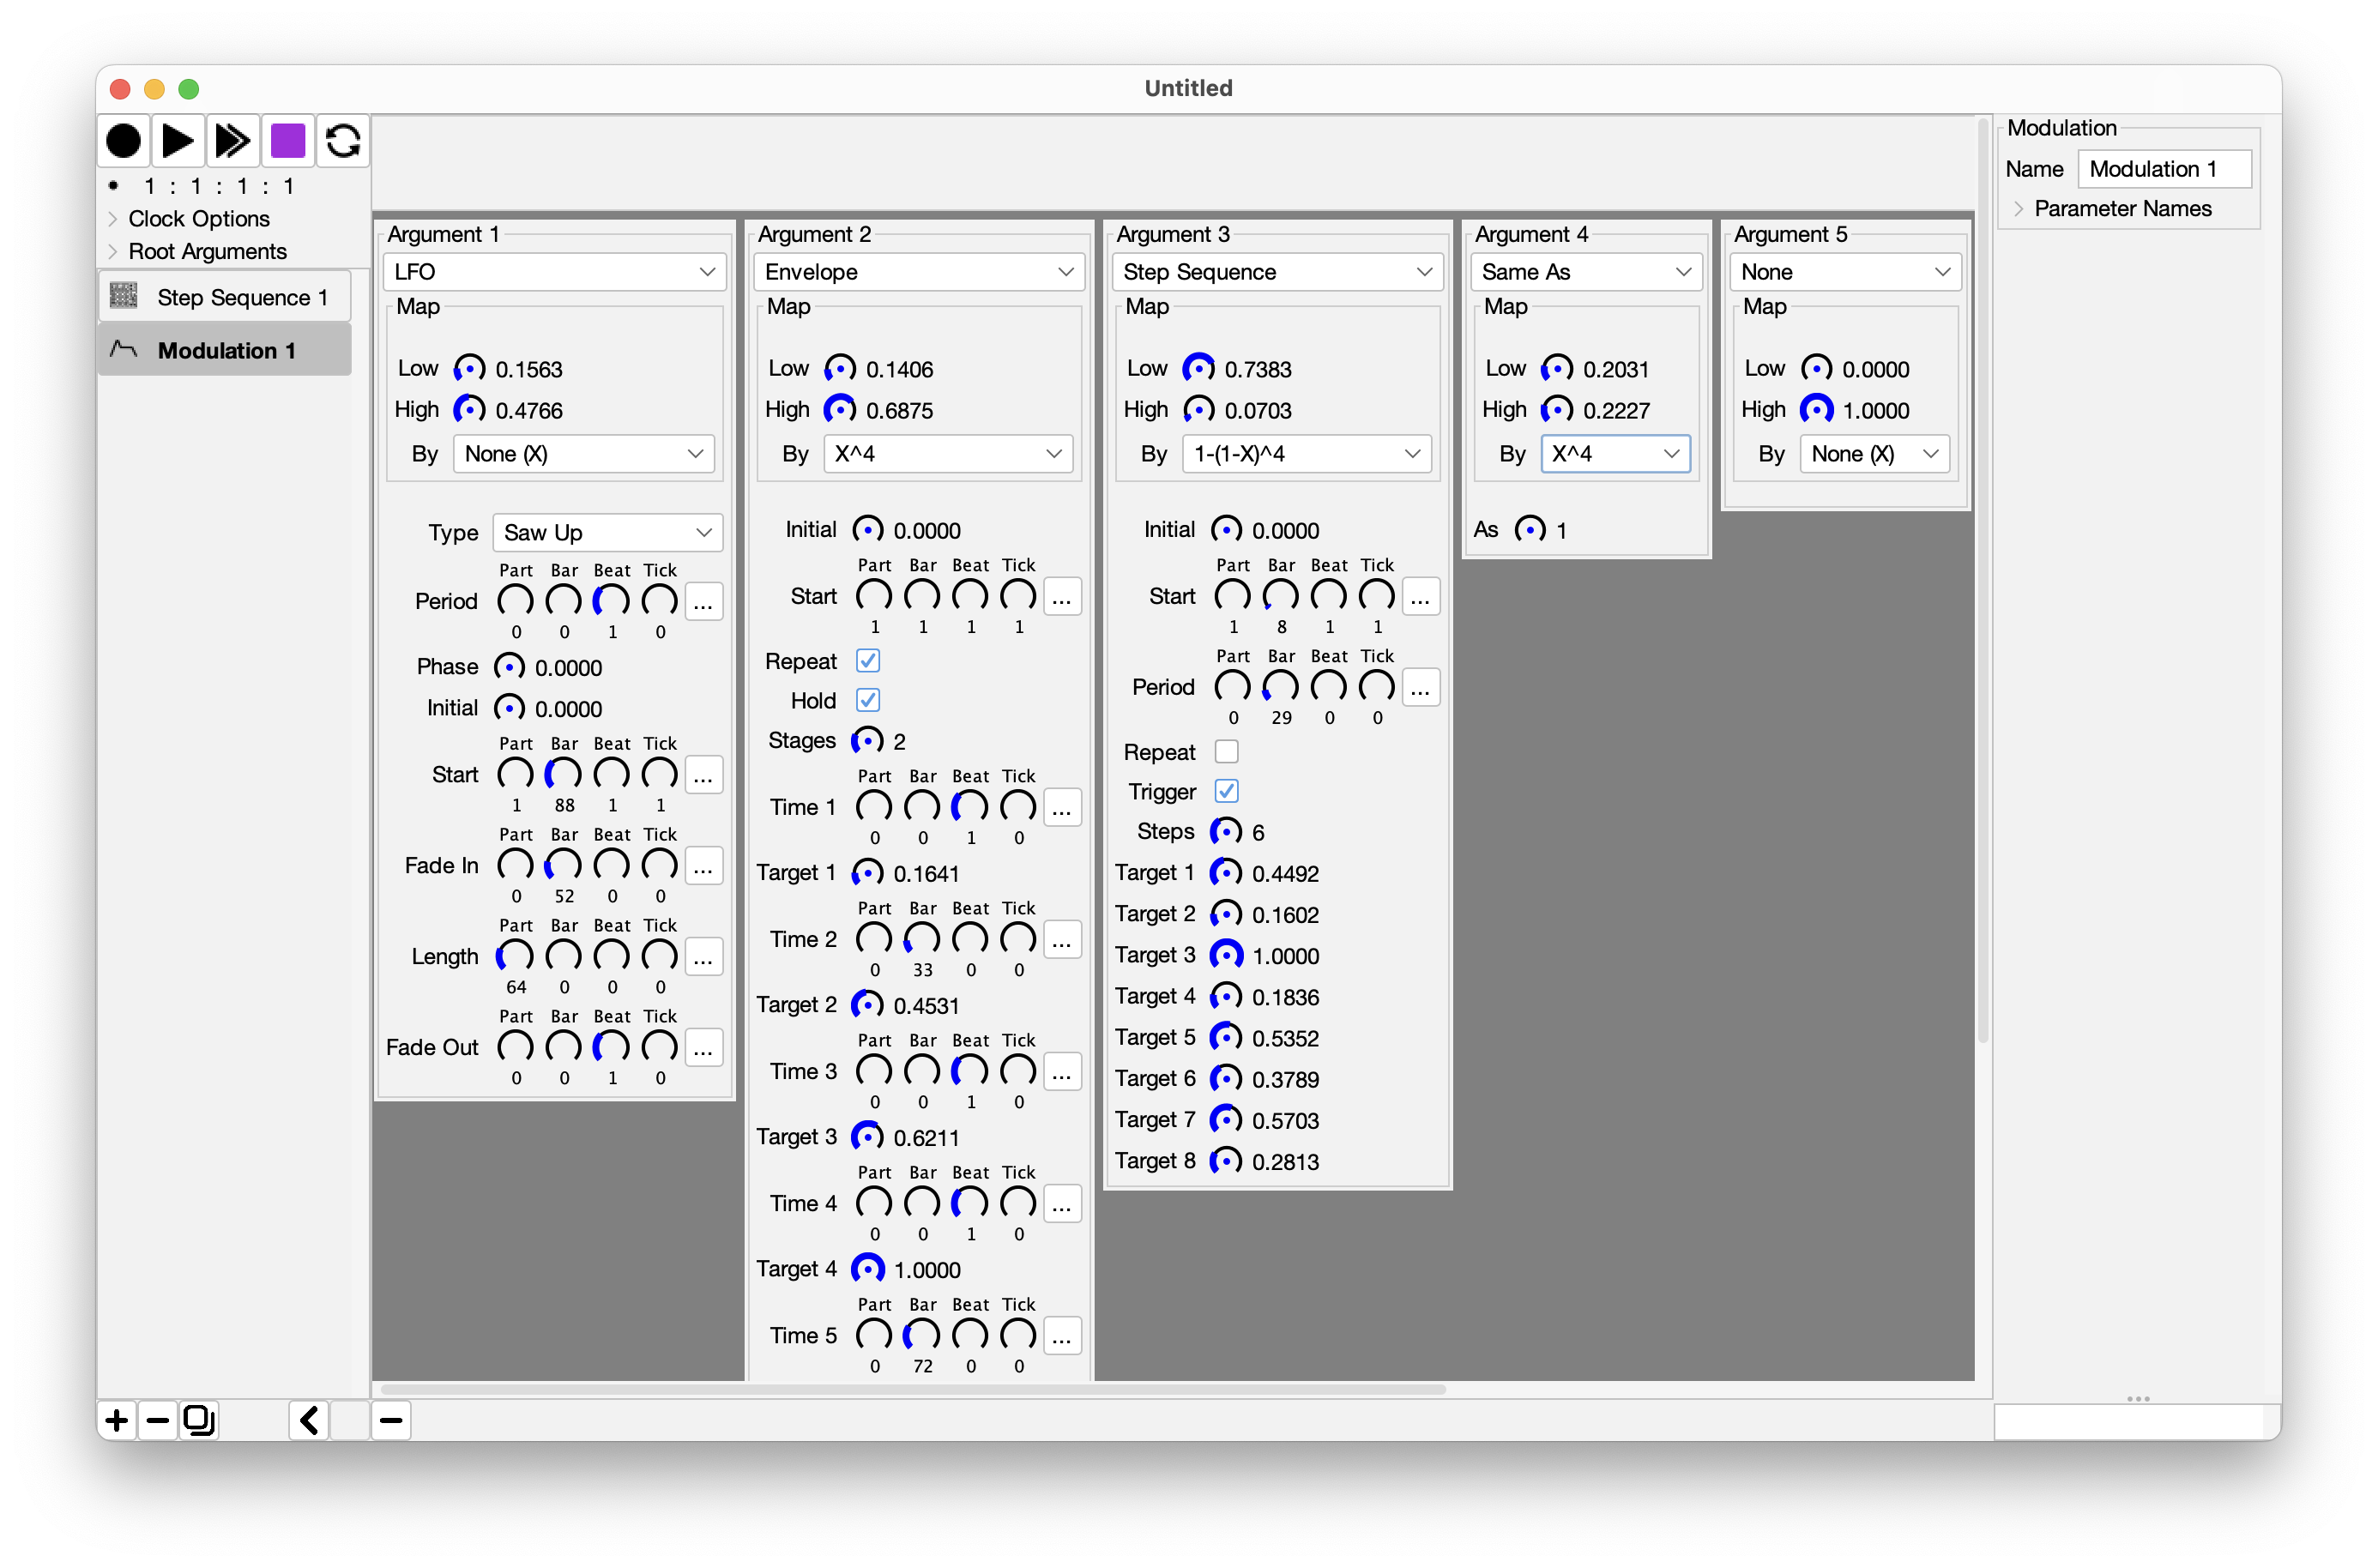
\includegraphics[width=6.5in]{Modulation}
\vspace{-2em}
\caption{Modulation Motif.}
\label{filter}
\end{figure}

\subsection{Modulation}

Modulation doesn't make any sound on its own, but it's not a MIDI filter.  Rather, it take a single child and provides some ways for you to modify the child's {\bf parameters}.

Note that, like Filter and Arpeggio, Modulation requires a single child to operate on, or else it does nothing!

Before we go any further, it might be helpful for you to read Section~\ref{parameters}, which discusses parameters.  In short: each motif has eight parameters, each of which can be set to any value from 0.0 to 1.0.  Many dials in a motif can be the value of one of the motif's parameters.  Furthermore, in the child's parent, you can modify the parameters of a child (from a parent's perspective, a child's parameters are called its {\bf arguments}).  If you don't, by default the settings of a motif's parameters are automatically set its parent's own parameters. This all allows you to change one or more dial settings in a child, or a deep descendant, or many of children or descendants at the same time, by setting a parent or ancestor's parameter values.

In most motifs you can directly set a child's arguments to values as you see fit, or to random values.  And Select lets you set its own parameters via big Dials, or via MIDI CC messages (Seq's root parameters can also be set via MIDI CC messages).  But {\bf Modulation} goes much further: it lets you change the parameters of a child via an automated modulation procedure such as a Low Frequency Oscillator (LFO), Envelope Generator, or a simple parameter Step Sequencer.  This gives you a way to change the parameters of a child automatically over time.


\paragraph{Mapping}

After the parameter value is determined by the automatic modulator you have chosen, it is passed through a {\bf mapping function} before it is finally set.  This allows you to scale the value to within a range of your choosing, invert it, and warp it using certain warping functions.

Your parameter value, output by the modulation function, has a range of 0.0 to 1.0.  We first warp it, using one of the following functions:

\begin{itemize}
\item {\bf None} (\(X\))\qquad No warping occurs.
\item \(X^2\)\qquad The argument is squared.
\item \(X^4\)\qquad The argument is squared twice.
\item \(1-(1-X)^2\)\qquad The argument is inverted, the squared, then inverted again.  This looks a little like subjecting it to a square root.
\item \(1-(1-X)^4\)\qquad The argument is inverted, the squared twice, then inverted again.  This looks a little like subjecting it to a square root twice.
\end{itemize}

After warping, the parameter still has a range from 0.0 to 1.0.  We then scale it to a new range from {\bf Low} to {\bf High}.  Note that {\bf Low} can be {\it higher than} {\bf High}: in this case the parameter range is inverted.

After all this mapping, the parameter is then passed to the Child.

\paragraph{Modulation Functions}

At present, Modulation has five automated modulation functions available:

\begin{itemize}
\item {\bf None}\qquad No automation.
\item {\bf LFO}\qquad The argument is modulated over time using a {\bf low-frequency oscillator}, which produces a repeating function.
\item {\bf Envelope}\qquad The argument is modulated over time using an {\bf envelope} with up to eight stages.
\item {\bf Step}\qquad The argument is modulated over time using a {\bf parameter step sequencer} with up to eight stages.
\item {\bf Constant}\qquad The argument is fixed to a constant value.
\item {\bf Same}\qquad The argument is set to the same value as some earlier modulation function.
\end{itemize}

We'll describe these next in detail.  More modulators are planned for the future.  

At the end of this list is {\bf Copy From...}, where you can ask that both the Modulation Function and the Mapping for a given Argument be copied exactly from another Argument.


\paragraph{None}

No modulation occurs.  The value of argument \(X\) in the child is set to the equivalent parameter \(X\) in the Modulation parent.  However, the argument is optionally mapped first.

\paragraph{LFO}

The value of argument \(X\) is set to the output of an LFO.  The LFO has the following parameters:

\begin{itemize}
\item {\bf Type}\qquad The LFO wave.  This can be Saw Up, Saw Down, Square, Triangle, Sine, Random, and S\&H (Random Sample and Hold).  Random works by selecting a random target position from 0.0 to 1.0 and slowly moving linearly to reach that position by the end of the period, at which it picks a new random target position and repeats.  S\&H works similarly, but it doesn't move: it just holds at its previous target position until the period is completed, at which point it jumps to the new target position.
\item {\bf Period}\qquad The length of one repetition of the wave, in time steps.
\item {\bf Phase / Var}\qquad For the {\bf Random} and {\bf Sample and Hold (S\&H)} wave types, this defines the {\bf Variance}, that is, how wide a swing in randomness is used when computing the next target location.  For all other wavetypes, this defines the {\bf initial phase} of the wave, ranging from 0.0 to 1.0.
\item {\bf Initial}\qquad The initial value of the LFO.   The LFO outputs this until it reaches its {\bf Start} time.
\item {\bf Start}\qquad The LFO's start time.  The LFO doesn't begin operating until this time: instead it sets the argument to {\bf Initial}.
\item {\bf Fade In}\qquad After the LFO's start time, the LFO gradually fades in from the initial value to the full range from 0.0 to 10.  This is done over the Fade In period: this is a time interval, not a specific time step.
\item {\bf Length}\qquad After the fade in has completed, the LFO will run for the Length.  This is a time interval, not a specific time step.
\item {\bf Fade Out}\qquad After the length has completed, the LFO will fade back out to the Initial value over this period.  This is a time interval, not a specific time step.  After the Fade Out is completed, the LFO will simply set the argument to the Initial value again.
\end{itemize}

LFO can also be used to randomize a parameter at a constant rate (unlike the {\it random parameter}, which is only set when the motif is reset or looped).  Set the type to Random, the period to your desired rate, and the mapping min and max to your desired random bounds.

\paragraph{Envelope}

The value of argument \(X\) is set to the output of an up to eight stage envelope with the following parameters:

\begin{itemize}
\item {\bf Initial}\qquad The initial value of the envelope.   The envelope outputs this until it reaches its {\bf Start} time.
\item {\bf Start}\qquad The envelope's start time.  The envelope doesn't begin operating until this time: instead it sets the argument to {\bf Initial}.
\item {\bf Stages}\qquad The number of stages in the envelope.
\item {\bf Time \textit{n}}\qquad The length of time for stage \(n\).  This is a time interval, not a specific time step.
\item {\bf Target \textit{n}}\qquad The target value for stage \(n\).  During its time interval, the envelope will gradually move from the previous target value (or from the initial value) to this new target value.
\item {\bf Repeat \textit{n}}\qquad When checked, the envelope will loop: when it finishes its last stage, it will go back to its first stage and continue from there.
\item {\bf Hold \textit{n}}\qquad When checked, the envelope will act like a {\bf Sample and Hold}: it will not gradually move towards its target value, but rather will stay at its previous target value (or at the initial value) until the stage is completed, at which time it will suddenly jump to the new target value..
\end{itemize}

\paragraph{Step Sequence}

This is much like a simplified Envelope with Hold: where each stage has the same duration.   We call these stages {\bf steps}.

\begin{itemize}
\item {\bf Initial}\qquad The initial value of the step sequencer.   The step sequencer outputs this until it reaches its {\bf Start} time.
\item {\bf Start}\qquad The step sequencer's start time.  The step sequencer doesn't begin operating until this time: instead it sets the argument to {\bf Initial}.
\item {\bf Step Length}\qquad The length of a single step.  This is a time interval, not a specific time step.
\item {\bf Steps}\qquad The number of steps in the envelope.
\item {\bf Step \textit{n}}\qquad The value of Step \(n\).  When in Step \(n\), the argument is set to this value.
\item {\bf Repeat \textit{n}}\qquad When checked, the step sequencer will loop: when it finishes its last step, it will go back to its first step and continue from there.
\item {\bf Trigger \textit{n}}\qquad When checked, the step sequence will not output the given when it reaches Step \(n\).  Rather, if the value is non-zero it will issue a short one-time-step burst of 1.0, then output 0.0 for the rest of the step time.  If the value is zero, it will always output 0.0 for the step time.  This is a {\bf trigger}: a short burst of 1.0 to indicate a trigger has occurred along the argument.  See the {\bf Series} motif for an example use of a trigger.
\end{itemize}

\paragraph{Constant}

This indicates that parameter is fixed to a certain {\bf constant value}.  Mapping still occurs, but it's not very useful.

\paragraph{Same}

This indicates that the modulation function for this argument (let's call it \(m\) is the same as the one for some other argument \(n\). Note that \(n\) must be set to {\bf less than} \(m\), or Same will indicate that the value is {\bf Invalid}, and will act just like {\bf None}.  Mapping still occurs regardless: thus Same can have a different mapping from the Node that it is the Same as.

\paragraph{Combining Modulations}

If you have a Modulation set up as a child to a Modulation, you can combine modulations on the same parameter.  For example, let's say you wanted to do an LFO until an envelope started, and when the envelope finished, you continued the LFO.  You create an LFO in the parent Modulation for parameter X, going all the time.  In the child Modulation for parameter X, you create an envelope which is delayed to start a while later.  Set the Initial value for the child Modulation to be {\it Param X} rather than a fixed number.  Add an additional stage at the end of the envelope.  Set its target value to be {\it Param X} as well.  Finally, set the time for the additional stage to be however long you'd like to fade from the envelope's termination to the LFO again.

You can do tricks like this for any combination of modulation methods.

\paragraph{Parameterization}

As usual, many Modulation features can be {\bf Parameterized} by double-clicking on the dials.  For more on parameterization, see Section~\ref{parameters}, (\textbf{\textit{Parameterized Control of MIDI Data}}).

\paragraph{Child Repeats}

As is the case for Serial, you can specify the number of times the child will repeat (loop) beyond its initial iteration before the Modulation determines that it has finished.

\paragraph{Child MIDI}

Like a number of other motifs, Modulation lets you modulate the rate, transpose, gain, and out of your (sole) child.  There is a difference however.  If you set the rate, transpose, or gain to a {\it parameter}, keep in mind that the whole point of Modulation is to modulate {\it its own parameters}, which are normally passed down to the child.  However these parameters that Modulation is modulating will {\it also} affect your Child MIDI settings.  This is by design: if for example you set your Child's MIDI gain to Param 1, then if you set up an Envelope on Argument 1, it will modulate that gain!





\clearpage\subsection{Motifs Planned for the Future}

At present we have a few motifs planned:

\begin{itemize}
\item A Motif for individual notes, or chords
\item Recorded automated modulation changes via a CC.
\item Possibly a Motif which does Live Coding using some programming language
\end{itemize}

\clearpage

\begin{figure}[t]
\centering
\includegraphics[width=6.5in]{Macro}
\vspace{-3em}
\caption{A Macro with Two Macro Children.}
\label{macro}
\end{figure}

\section{Macros and Macro Children}
\label{macros}

A {\bf Macro} is a whole Seq sequence DAG bundled up into a single Motif.  When the Motif is played, the underlying sequence is played until it is finished.

To create a basic Macro, you first save our your sequence.  (Remember that the sequence is saved out starting at the Motif Root, ignoring its parents and other non-descendant Motifs.)  Then you add a Macro to the Motif List and when you do it will prompt you to load that sequence into the Macro.    When you play the Macro, its stored sequence is played as-is.

This has some usefulness, but Macro can go further than this.  You can add special Motifs to your sequence called {\bf Macro Children}.  A Macro Child has a single Inspector feature: its {\bf Name}: come up with a good name for it.  If you have Macro Children in the sequence you have saved out, they become temporary placeholders for actual Children of the Macro in  your main sequence.

This means that if you had three Macro Children nodes in your macro's internal sequence for example, then the Macro itself will take up to three Children.  As the Macro is playing, it will reach its Macro Children nodes, and instead of playing them, the Macro will play the corresponding Child attached to it.  Figure~\ref{macro} shows a Macro loaded that had two Macro Children nodes inside, and thus has two slots for Children, which we have populated with a Notes and a Series from the Macro List respectively.

What's the point of this?  It allows you to use Macros to create patterns or templates, and then populate the templates with different Children as you see fit later on. 

The Child slots of a Macro are populated in the usual way: by dragging from the Motif List.  You can also clear a slot by pressing the {\bf Delete Button} below.  You can change the Name of the underlying Macro Child node: this is now the {\bf nickname} of the Child in its Inspector.

\clearpage\section{Parameterization}
\label{parameters}

Many of the dials on Seq's motifs are {\bf Parameterizable}.  This means that instead of setting a dial to a value, you can arrange for it to be changed elsewhere in Seq by something else (another dial, a MIDI message, an automatic mechanism).  This makes possible many things.  For example, you could:

\begin{itemize}
\item Control a dial from a remote MIDI CC.
\item Control multiple dials in a motif\,---\,for example, the velocity of four different notes\,---\,together from the same dial elsewhere.
\item Control several dials in different motifs\,---\,for example, the swing of three different Step Sequencers\,---\,together from the same dial elsewhere.
\item Set a dial to a random value before its motif begins playing.
\item Control dials dynamically from an automatic mechanism such as an LFO or an envelope.
\item Send a {\bf trigger} to a motif, such as a telling a Series to stop repeating one of its children.
\end{itemize}


\paragraph{Parameters} Each Motif has eight {\bf Parameters}.   Just before the Motif's parent steps the Motif to advance it a little bit, the parent has the opportunity to change the values of any of those Parameters.  The parent can change them to any value from 0.0 to 1.0, or it can set them to any of the current values of the parent's {\it own Parameters}.  (In fact, by default the value of Parameter \(X\) in a Motif is set to the value of Parameter \(X\) in its parent).

Normally changing a motif's parameter does nothing.  But many of the dials you see in a Motif can be {\bf bound} to one of those parameters, meaning that if that parameter is changed, the dial will also be changed.  This allows parents, or ancestors, to change one or more dials in their children or descendants.  Multiple dials can be bound to the same parameter, meaning that by changing a single parameter, a parent can simultaneously affect a number of Dials, even spread across multiple child Motifs.

\paragraph{Arguments}

From the child motif's perspective, a parameter\,---\,the thing it may have connected its dials to\,---\,is unsurprisingly called a {\bf parameter}.  But from the parent's perspective, changing or setting one of its child's parameters is called changing an {\bf argument} in the child.  This terminology is borrowed from computer science, because to a computer programmer, motifs may be thought of as functions (or methods or procedures), and functions have arguments (set by the caller of the function) and parameters (read inside the function).


\begin{wrapfigure}{r}{1.25in}
\vspace{-4em}
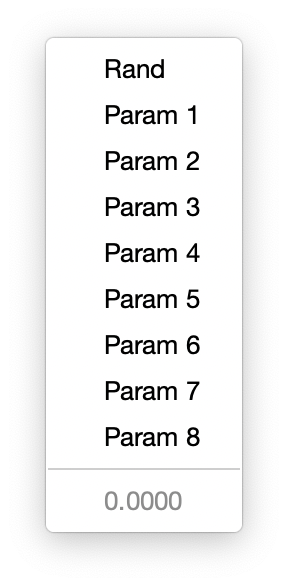
\includegraphics[width=1.2in]{params}
\vspace{-1em}
\caption{A Parameter Menu}
\label{params}
\vspace{-3em}
\end{wrapfigure}


\paragraph{Binding a Dial to a Parameter} You can tell that a dial can be bound to a parameter because it has a little red or blue {\bf dot} in the middle of it.  You bind the dial by double-clicking on it.  This brings up a pop-up menu as shown in Figure~\ref{params} at right.  Here you can bind the dial to any of its motif's parameters, here shown as {\bf Param~1 ... Param~8}, or to the motif's random parameter ({\bf rand}).

After you have bound a dial to a parameter, the dial's will go gray, the dot will go red, and the name of the parameter will be shown along side it. If you would like to break the binding and go back to setting the dial to a fixed value, just turn the knob. 

\paragraph{Changing the Parameter Name} Don't like the name {\bf Param 1}?  Want something more descriptive so you can remember what the heck that parameter is for?  Many motif inspectors have a {\bf Parameter Names} section where you can change the names of all eight of the motif's parameters.  You will have to click on the Parameter Names to open it up.

\begin{wrapfigure}{r}{2.25in}
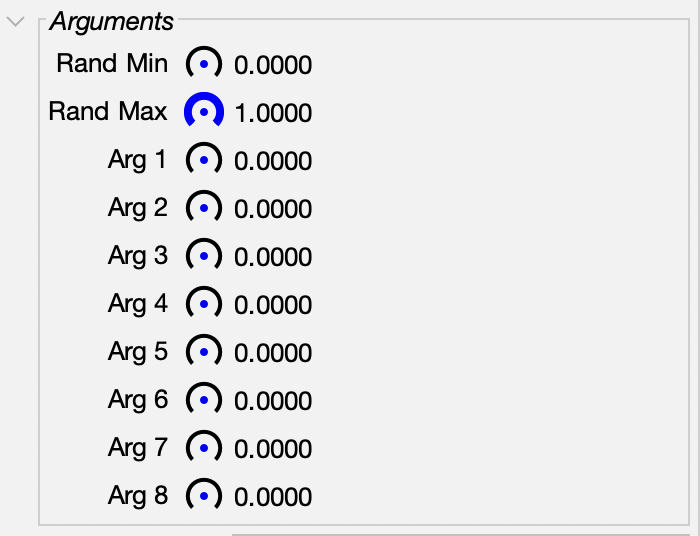
\includegraphics[width=2.25in]{arguments}
%\vspace{-2em}
\caption{Arguments List.}
\label{arguments}
\end{wrapfigure}

\paragraph{Changing a Child's Argument Values from the Parent} Many parent motifs can change the arguments of their children.  If you click on a child motif, its inspector may have a region called {\bf Arguments} (you will have to click on it to open it up).  You can see the Arguments list in Figure~\ref{arguments} at right.  Here you can set the values of the arguments sent to the child's parameters.  You can also set the minimum and maximum bounds of the child's random parameter.   

By default the arguments are called {\bf Arg 1 ... Arg 8}.  But if you provide names for the child's parameters, they will appear here instead.  

Note that these dials are themselves parameterizable: this means you can bind the child's parameters to the parent's parameters (and so on up the chain).  In fact by default the arguments are bound to the parent's parameters already.  For example, {\bf Arg 1} is set to the parent's {\bf Param 1} and so on.

Not all parents can change their child parameters even though they have children.  Notably the Arpeggio, Modulation, and Filter motifs cannot change the parameters of their sole child.  Instead the child's parameters are simply set to their own parameters.  

\paragraph{The Random Parameter} In addition to the eight parameters, the Motif also has an additional {\bf Random Parameter}.  This parameter is set to a random value once each time a Motif is started or looped.  This value is not changed while the Motif is stepped.  Dials can also be bound to this value.  Additionally, a child's arguments can be bound to the parent's own random value.

A parent cannot change the value of its child's random parameter: it is set to a random value.  But the parent can change the {\bf minimum and maximum bounds} from which the random value is selected.  These bounds, like any other parameter, can be set to fixed values or bound to the parent's own parameters or to its random parameter.

\paragraph{A Warning about Child Arguments}

Consider the Series motif. Each of its children can have (for example) Initial Repeats.  These can be bound to parameters.  But note that these features are {\it not features of the Child}: they are features of the {\it parent Series}, and thus they are bound to the Series's parameters, not to the Child parameters.  This can be a little confusing.  In short, if a feature appears anywhere in {\it any Inspector} associated with a Motif (the Motif Inspector, one of its Child inspectors, etc.), that feature {\it belongs to the Motif} when it comes to parameterization.  It doesn't belong to the Child.

\paragraph{Triggers} The Series and Automaton motifs have special options to repeat children forever until receiving a {\bf trigger} on Parameter 8.  What is a trigger?  A trigger on Parameter 8 is, well, triggered, when Parameter 8 changes from a value \(< 0.5\) to a value \(\geq 0.5\). 


\begin{wrapfigure}{r}{1.25in}
\vspace{-1em}
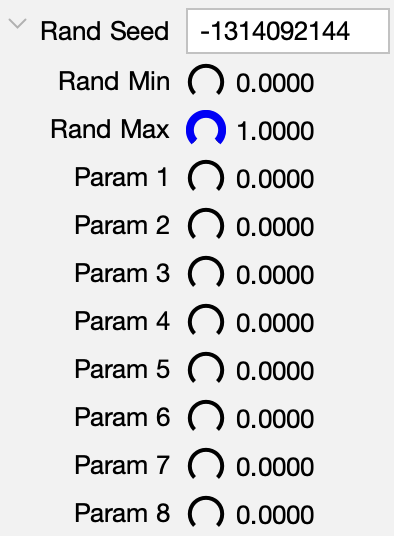
\includegraphics[width=1.25in]{rootarguments}
%\vspace{-2em}
\caption{Root Arguments with default settings.}
\vspace{-4em}
\label{rootarguments}
\end{wrapfigure}

A parameter is just a real-valued number between 0.0 and 1.0.  But of course many Seq dials don't go 0.0 to 1.0: they go 0...127 or 0...4 or whatnot.  These ranges are mapped  as appropriate.  This can make setting the parameter a pain, but you can tell what the appropriate mapping for a parameterizable dial is but double-clicking on it: at the bottom of the pop-up menu is a grayed-out value. That's the real-valued parameter value that would correspond to the current feature value.    


\paragraph{The Root Arguments}  If the Root Motif has bound some dials to its parameters, where are those arguments set?  They're set in the Root Arguments, located below the Transport (the play and record buttons, etc.)  See Figure~\ref{rootarguments} at right.  This is also where you can change the {\bf Random Seed} of your sequence.  If you change the random seed, the random number generator will produce a different sequence of numbers next time.

For each root argument, you can also set a {\bf Control Change} or {\bf CC} parameter to allow an external controller to change the argument in real-time as you see fit.  To do this, you'll need to specify the {\bf CC In} device from which these CC messages will come.  When you start playing a sequence, the root arguments will be set to the fixed values you specified: but if you afterwards send CC messages, they will be changed.  If you don't want to use this feature, set  {\bf CC In} to {\it None}: it's a bit more efficient.

\paragraph{Macro Root Arguments} You'll note a dot in the center of each of the root arguments, and you thus by double-clicking on it you can change each argument to say {\it Macro}.  This only has an effect once the root is saved out as a macro: otherwise, setting the argument to {\it Macro} is the same as setting it to 0.

When you save out a macro, the parameters of the macro's root can be set to fixed values (the root arguments) or they can be set to {\it Macro}.  This means that the root's parameter will be set to whatever the Macro's parameter values are set to when you use the Macro from its parents in the outer sequence.  For example, if Root Parameter 3 is set to {\it Macro}, then when used in a Macro, Root Parameter 3 will be bound to the Macro's own Parameter 3.  Thus you can either fix the parameters to values or you can allow them to be customized by the Macro's parents.

\paragraph{How Parameterization Works}
To understand how parameterization is updated, let's first make sure we understand how  parent motif instructs a child to play.  First, before any playing, the parent {\bf resets} its child to set its time position to 0 and to initialize it.  Then each timestep (192 times per beat), when the parent itself is being {\bf pulsed} by {\it its parent}, it in turn pulses the child to advance it.  At some point the child will tell its parent that it has {\bf finished}, or for some other reason the parent decides to stop playing the child.  At this point the parent will {\bf stop} the child\,---\,it will tell the child that the playing has ended.  Then the parent can either go about doing other things, or it can {\bf loop back} and replay the child as it sees fit.  If it replays the child, it once again resets it and starts the process again.  So in short, it does:

Woven in-between these steps are opportunities for the parent to set parameters in the child.    Each motif has eight parameters that its parent can chance.  Additionally, the motif has a {\bf random value} which is selected (at random!) when the child starts playing: the parent does not set this directly, but it can change the minimum and maximum values from which the random value is chosen.  Adding the parameter-setting stages, we have: 

\begin{enumerate}
\item Before playing, reset the child.
\item Before playing, the child generates its random value.
\item Each time the parent is pulsed, as it sees fit:
\begin{enumerate}
\item Change the child's parameters as it sees fit.
\item Pulse the child
\end{enumerate}
\item After all playing has finished, stop the child.
\item Either continue doing something else, or loop back to step 1 as it sees fit. 
\end{enumerate}

Note that looping back will change the random value to a new number.

\paragraph{What Motifs are Parameterizable?}

\begin{itemize}
\item {\bf Notes} and {\bf Step Sequence} have dials that can be set to parameters, and you can name the parameters.
\item {\bf Series, Parallel, Select, Filter, Modulation} and {\bf Automaton} have dials that can be set to parameters, and you can name the parameters.  Furthermore these motifs have children, and you can change each child's arguments.
\item The parameters of {\bf Silence} don't do anything, because these motifs have no parameterizable dials.    You can't name the parameters for the same reason.
\item The parameters of {\bf Macro Child} are simply passed down to the Motif assigned to the Macro Child when you are using its Macro.  You can't name the parameters.
\item {\bf Arpeggio} has no parameterizable dials.   Is parameters are simply set to pass data down to the parameters of its sole child.  You can't name them: their names will be the names of the parameters of its sole child.
\item {\bf Macro} has no parameterizable dials.  When you change the arguments of a Macro, these values are passed down to the root Motif of its internal sequence.  Alternatively you can set Macro to always send the same fixed values to its root Motif, ignoring the arguments it receives.  This choice is made per-argument when you save the Macro out.  See {\bf Root Macro Parameters} above.
\end{itemize}

\subsection{Parameterized Control of MIDI Data in Series}
\label{mididata}

The {\bf Series} motif has a trick up it sleeve: the ability to output parameters as MIDI CC, NRPN, RPN, Pitch Bend, or Aftertouch. You can find this by clicking on {\bf MIDI Parameters} in the Series inspector.  This will expand to {\bf Param 1} through {\bf 8}, along with {\bf Out}.  For each Param you can select a Type (such as CC or NRPN), and then a number if appropriate.  

Let's do an example.  First set Param 1's Type to CC.  This reveals a Dial you can set to specify the CC number (from 0--127).  Let's say we set this to 5.  Finally let's set Out to the output device which will receive the CC MIDI messages.

Now, whenever the Series is playing, if its incoming Parameter 1 has changed in value, it will be mapped to a CC value and emitted out CC 5.  Parameters have values from 0.0 to 1.0, whereas CC values range from 0 to 127.  So for example if Parameter 1 changes to 0.5, this will be mapped to 63, and so Seq will emit a CC message number 5 with a value of 63.

The rate at which MIDI data is output is chosen by the {\bf Rate} parameter.  MIDI data will only be output if the parameter has changed since the last time MIDI data was output.

The following MIDI output types are available for each Parameter.

\begin{itemize} 
\item {\bf None}\quad Nothing is emitted.
\item {\bf CC (Control Change)}\quad You specify the CC number (0--127).  Incoming parameters will be mapped to CC values (also 0--127).
\item {\bf 14-bit CC}\quad You specify the CC parameter (0--31).  Incoming parameters will be mapped to 14-bit CC values (ranging 0--16383).
\item {\bf NRPN}\quad You specify the NRPN parameter (0--16383) with two dials: the left one specifies the coarse value or MSB, and the right one specifies the LSB.  The final NRPN number is displayed.  Incoming parameters will be mapped to NRPN values (also 0--16383).
\item {\bf Coarse NRPN}\quad You specify the NRPN parameter (0--16383) with two dials: the left one specifies the coarse value or MSB, and the right one specifies the LSB.  The final NRPN number is displayed.  Incoming parameters will be mapped to NRPN coarse (or MSB-only) values (0--127).
\item {\bf RPN}\quad You specify the RPN parameter (0--16383) with two dials: the left one specifies the coarse value or MSB, and the right one specifies the LSB.  The final RPN number is displayed.  Incoming parameters will be mapped to RPN values (also 0--16383).
\item {\bf Pitch Bend}\quad Incoming parameters will be mapped to Pitch Bend values (\(-8192\)--8191).  Thus if you set the Parameter to 0.5, then this will map to 0.
\item {\bf Channel Aftertouch}\quad Incoming parameters will be mapped to Channel Aftertouch values (0--127).
\end{itemize}

\subsection{Select's Overriding of Parameters}
\label{selectparameters}

Select has a performance option where it can override its own parameters, setting them to values chosen by Select and not by its parent.  Why would you want to do this?  Because the parameters of various children of Select can be bound to those parameters.  This allows you to change the parameters of children in real-time via a Big Dial, a Joystick, or a MIDI CC message from a remote controller.

\paragraph{Overriding a Parameter}

In the {\bf Dial Parameters} region of Select's Inspector, check the box of the parameter you'd like to override (Dial 1 through Dial 8, corresponding to Parameters 1 through 8).  When you do so, note that the grid will change to reveal the Big Dial for that parameter.

Next, select a child, and in the Child Inspector, go to the Arguments section.  In there, change the corresponding Argument to be the Parameter.  For example, if you overrode Dial 3, and you want this to modify the Child's Argument 2, you'd set Arg 2 to Param 3.  

Now, when the Select is playing, you can change the value of this parameter of Dial 3 (for example), and it will update the Child's Parameter 2 to reflect this value in real-time.

You can set up multiple children this way to respond to Dial 3.

In fact, by default all children's parameters are just set to Select's parameters.  This means that if you turn on and change Dial 3, it will affect parameter 3 of every child.  So in most cases if you want to set a parameter, you're probably already set unless you want to change which parameter it is bound to.  In fact in most cases you might only want to {\it disconnect} a parameter from some child.

\paragraph{Using the Joystick}
Select provides an on-screen Joystick to control two different parameters just like the Big Knobs do.  To set up the Joystick, in the {\bf Dial Parameters} section of the Inspector, specify which two parameters should be assigned to the X and Y axes of the Joystick.

Opening the {\bf Joystick} section of the Inspector reveals the Joystick.  Move the Joystick around and the corresponding Parameter will be changed.  This will happen even if the Big Dial for that Parameter is not being displayed.

\paragraph{Attaching a Controller}
Instead of turning these Dials on the screen, you can turn them with a knob on your controller.  

First, override the parameter in question as described above.

Second, in the {\bf Dial Parameters} region of Select's Inspector, change the CC In device to the device corresponding to your controller.

Third, for each Dial you'd like controlled by the Controller, in the Dial Parameters region of Select's Inspector set the CC value of that Dial to the value you'll be sending from the Controller.

And you're done!  Changing knobs on the controller will change the Dial, which in turn will update the parameters of the Children you bound to it.

\section{Developing for Seq}

Seq is written in pure Java, and is designed to have a simple model, even if the graphical interface code is relatively elaborate.  The reason for this was that, ultimately, we hope Seq's model can be rearranged and customized by optimization and machine learning tools.  For now, it's just an unusual sequencer.

\begin{figure}[t]
\centering
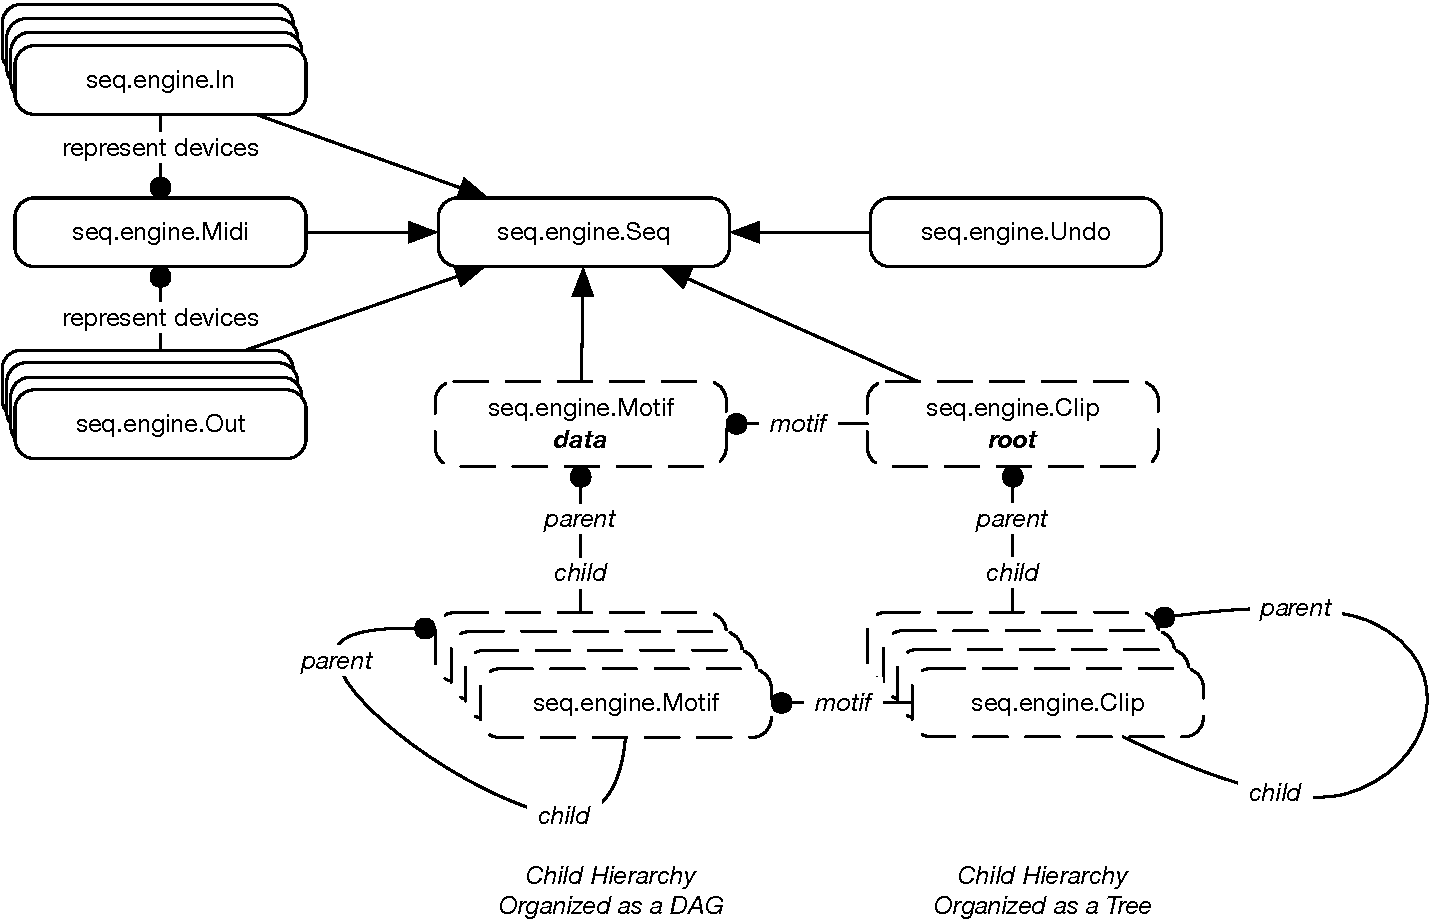
\includegraphics[width=4in]{model}
\caption{Model class relationships.}
\label{modeldev}
\end{figure}


\subsection{Model and Dynamic Runtime Overview}

The top-level class of Seq is {\sf seq.engine.Seq}\footnote{Well, that's not {\it quite} the case.  There's a small bootstrapping class called {\sf seq.Seq} so you can launch Seq as {\tt java seq.Seq}.}  Seq is a singleton object which contains the entire sequence.  It manages playing and recording the sequence,  as well loading and saving it, and stores the sequence model.  {\sf seq.engine.Seq} also contains the global lock, which synchronizes between playing / recording notes and modifying / displaying the sequence from the GUI.

Seq runs the MIDI subsystem, both sending and receiving.  The MIDI subsystem itself is managed by the class {\sf seq.engine.Midi}, which Seq owns.  Seq permits 16 outputs and 4 inputs.  Each output and input represent a combination of a MIDI Device, a MIDI channel, and a nickname given by the user.  These outputs and inputs are stored in 16 {\sf seq.engine.Out} and 4 {\sf seq.engine.In} objects respectively.

{\sf seq.engine.Seq} maintains the sequence using two separate data structures.  First, there is the {\bf Motif DAG}, which stores the model itself.  Second, there is the {\bf Clip Tree}, which manages dynamically changing data while the model is playing.  

Each of these graph structures contains an entry point where the sequence begins when you press play.  For the DAG, it's a {\sf seq.engine.Motif} object called {\bf data}.  For the Clip Tree, it's a corresponding {\sf seq.engine.Clip} called {\bf root}.  This is called the root simply because it's the entry point for the sequence: though for the Clip Tree, it {\it is} the root of the tree, the corresponding {\bf data} object isn't necessarily the root of the DAG at all (and there could be multiple roots).

The Motif DAG consists, at the bottom, of note-generating Motif objects such as Step Sequence or Notes.  Every Motif may have multiple parent Motifs which indicate how to group their children together to play them, such as in series or in parallel.  This DAG is loaded from and saved to a JSON structure using the {\sf seq.load()} and {\sf seq.save()} methods, which in turn call similar methods on each of the Motifs.

When the sequence is played, the {\sf seq.engine.Seq} prepares and resets playing data, then starts the clock (a {\sf java.util.Timer}\footnote{{\sf java.util.Timer} only has a resolution of 1ms.  That's pretty bad, but it's what we have to work with.  I can build a custom Timer using nanoTime rather than currentTimeMillis, but it only increases the resolution by about \(1.5\times\).  It's possible to build a timer using park and unpark, but it doesn't improve things much and is very computationally costly.  The fundamental issue is the typical multitasking time-slice of the operating system.}.  The clock calls {\sf Seq.step()} 192 times per beat (that is, 192 Parts Per Quarter-note, or PPQ) at the current BPM. {\sf step()} acquires the lock, then calls {\sf advance()} on the {\bf root}, which in turn calls {\sf process} on the root.  This kicks off the series of recursive calls to {\sf advance} and {\sf process} throughout the root's Clip Tree, which gives each {\sf sim.engine.Clip} in the tree a chance to advance itself forward one tick (1/192 PPQ).  When this process is done, Seq lets go of the lock.

Each {\sf sim.engine.Clip} is associated with a {\sf sim.engine.Motif} in the model, and each will consult with its Motif to determine what notes to play, which children Clips to create and how to process them, and so on..  But there may be many Clips playing the same Motif at the same time, due to parallelism in play.  Each of these Clips must maintain its own dynamic information (such as its current timestamp), so they have to be distinct from one another.  To do this, the Clip must be a tree: parents cannot share the same child, they have to have their own distinct children.  Obviously this tree can be much larger than the DAG.  However it does not have to all exist at once.  The Clips in the Clip Tree are generated as needed, and garbage collected when their subtrees are finished playing their portion of the sequence.  

While advancing forward, Clips will generate MIDI.  They do not directly emit MIDI to the operating system.  Rather, they send MIDI to their parents in the Clip Tree, who pass it to their parents, and so on.  Eventually the {\bf root} passes MIDI to Seq to process and emit to the operating system.  This procedure allows parents to filter or modify the MIDI of their children (as in the Filter and Arpeggio motifs).

A module {\it foo} in Seq would be stored in the Java package {\sf seq.motif.foo}, and commonly would consist of at least the three following items:

\begin{itemize}
\item A Motif called {\sf seq.motif.foo.Foo}, which defines the parameters of the module and its relationship to child Motifs if any
\item A Clip called {\sf seq.motif.foo.FooClip}, which performs the actions of the module when it is being played or recorded
\item The GUI classes for the module, discussed next.  These would be stored in the Java package {\sf seq.motif.foo.gui}
\end{itemize}

\begin{figure}[t]
\centering
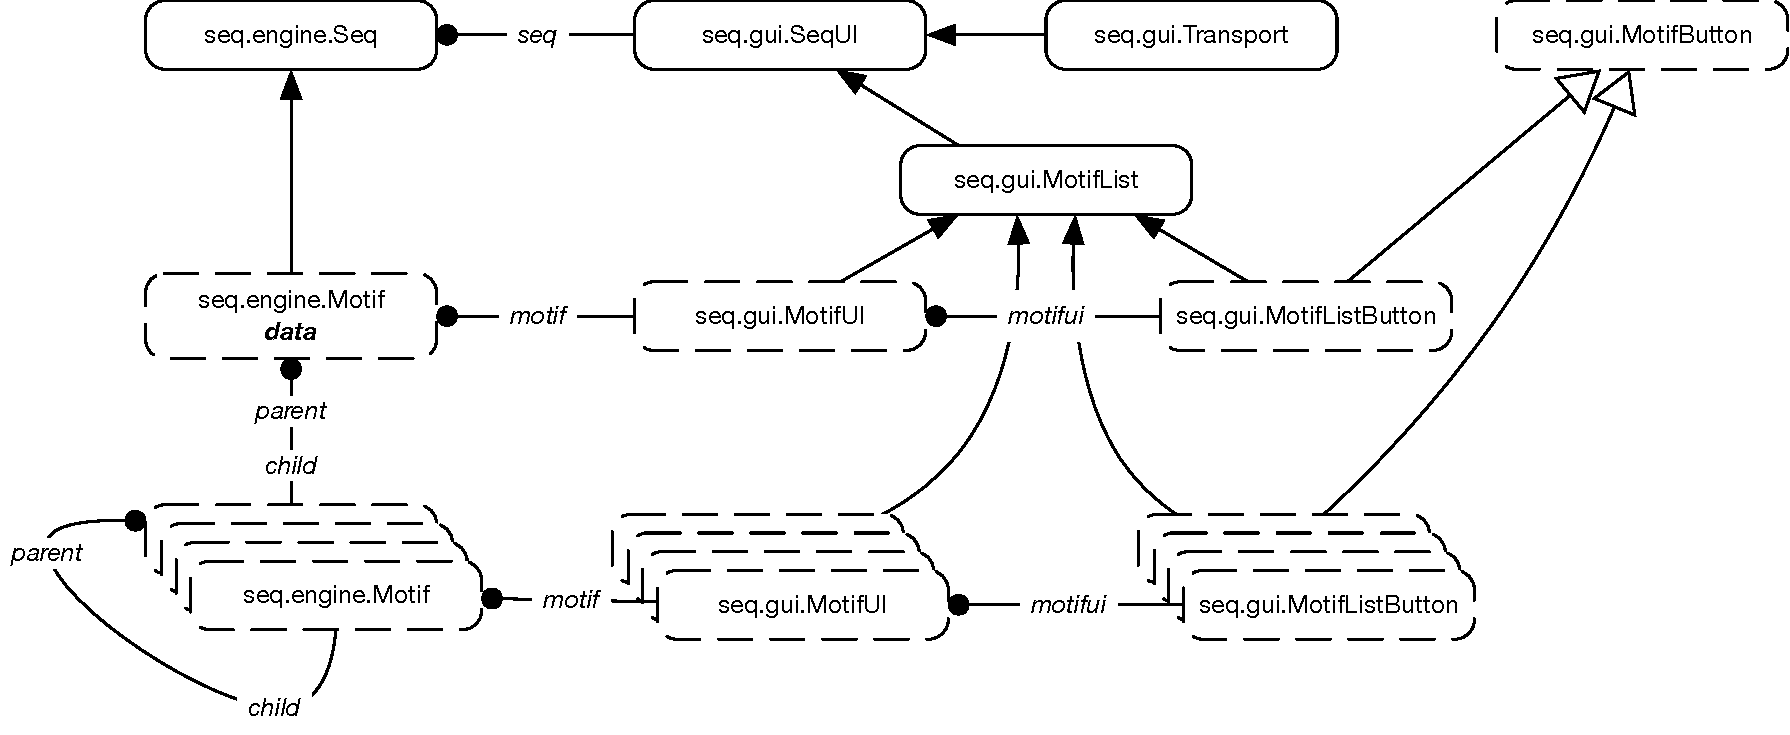
\includegraphics[width=5in]{gui}
\caption{GUI class relationships.}
\label{guidev}
\end{figure}


\subsection{Graphical Interface Overview}

The graphical interface is written entirely in Swing, using FlatLAF to define the look and feel.  The top-level GUI class is {\sf seq.gui.SeqUI}, which handles top-level application management and is the counterpart to {\sf seq.engine.Seq}.  SeqUI manages (most of) the menu, the main window, and all dialogs.  SeqUI manages playing and recording through an object it owns, {\sf seq.gui.Transport}.  This object handles all the transport buttons as well as the disclosure panel for the clock options.

SeqUI also manages the list of Motifs at the left of the window.  It does this through another object it owns, {\sf seq.gui.MotifList}.  MotifLIst not only displays the Motif buttons, but manages their creation, deletion, copying, ordering, and drag-and-drop into other Motifs.  The Motif buttons in the MotifList are drawn with {\sf seq.gui.MotifListButton}, which is a subclass of the more general {\sf seq.gui.MotifButton}.

\begin{figure}[t]
\centering
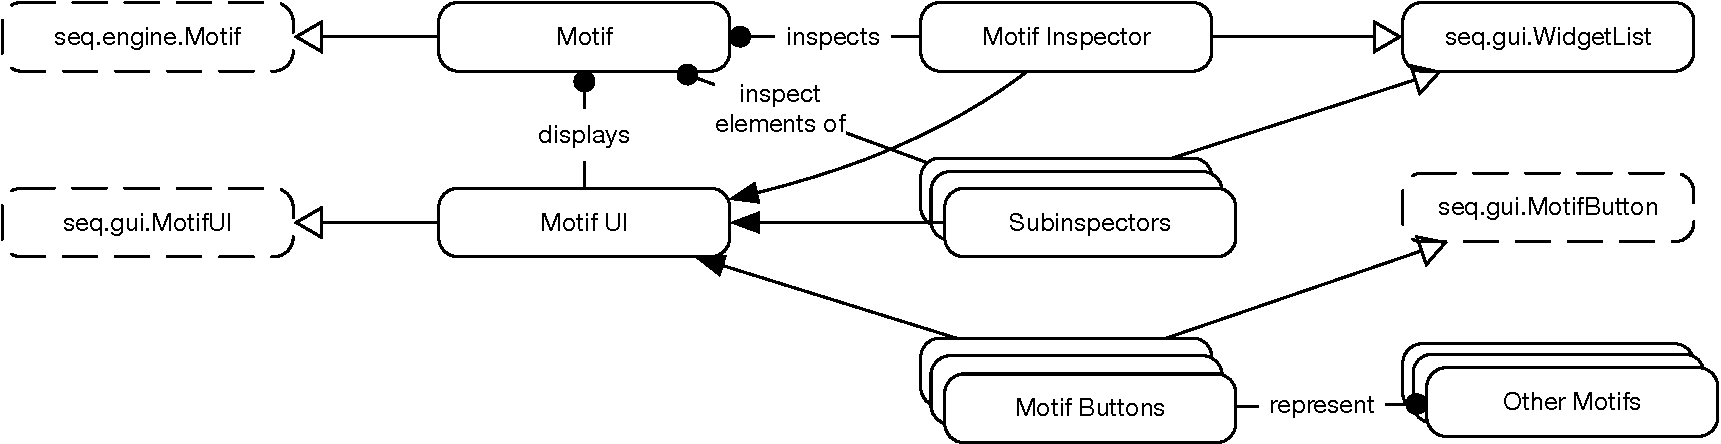
\includegraphics[width=5in]{inspectors}
\caption{MotifUI relationships.}
\label{inspectorsdev}
\end{figure}

SeqUI delegates the main drawing area and the inspector regions.  The main drawing area is handled by a subclass of {\sf seq.gui.MotifUI} which SeqUI creates when the appropriate MotifButton has been created or selected.  This class provides the main window region, and also provides the main structure for the inspectors.  Each MotifUI (and each MotifButton) is associated with a unique Motif.

MotifUIs generally build inspectors by subclassing from {\sf seq.gui.WidgetList}, a simple class for creating a labelled vertical list of elements.  Each MotifUI has its own primary inspector, and certain elements in the MotifUI will have their own subinspectors created when those elements are selected. 

Many Motifs have child Motifs, and MotifUIs represent these child Motifs with drag-and-drop objects which are subclasses of {\sf seq.gui.MotifButton}, just like {\sf seq.gui.MotifListButton} was.

The GUI subsystem for a module {\it foo} would be stored in the Java package {\sf seq.motif.foo.gui} and typically consist of:

\begin{itemize}
\item A MotifUI called {\sf seq.motif.foo.gui.FooUI}, which interacts with the Motif and Clip, draws the Motif, and dictates which inspectors will be used.
\item The primary inspector for the MotifUI, called {\sf seq.motif.foo.gui.FooInspector}
\item Any additional inspectors for subelements of the Motif
\item If the Motif has children, a subclass of MotifButton, likely called {\sf seq.motif.foo.gui.FooButton}, which displays those children.
\end{itemize}

\subsection{Common GUI Widgets}

To make your life easier, and to provide a consistent experience, Seq has a number of standard widgets which your MotifUI and inspectors may use:

\paragraph{seq.gui.WidgetList}  This is the superclass of inspectors, and is designed to make it easy to create labelled lists of JComponents.  Typically all the JComponents, and all their labels, are provided in the constructor; or you can provide them in a later {\sf build()} method.

\paragraph{seq.gui.SmallDial}  This is how Seq makes all of its dials.  SmallDial has a range from 0.0 to 1.0, which you initialize up front.  Then you override up to three methods.  {\sf setValue()} informs you that the user has just set the widget.  Typically you'll acquire the lock (see Locking later) to update the model.  {\sf getValue()} asks you what value to display.  Typically you'll acquire the lock (again, see Locking later) to read from the model.  And {\sf map()} asks how to print the data value next to the widget: by default this method formats its double value (0.0 to 1.0) as x.xxxx.

\paragraph{seq.gui.Dial}  A large version of SmallDial.

\paragraph{seq.gui.DisclosurePanel}  This is a JComponent which hides its children components until the user clicks on a ``\(>\)'', expanding it to display them.  If you provide it with its parent component, it will inform the parent when it has expanded so the parent can revalidate itself.

\paragraph{seq.gui.PushButton}  A convenient class for constructing a JButton which performs an action, or which produces a pop-up menu and performs an action based on what is selected.

\paragraph{seq.gui.StringField}  A convenient class for editing text strings.  When the user has edited a string, StringField will call the method {\sf setValue()}, which you override, so you can update the Motif data or whatnot.  Similarly to request the latest string from you to display, StringField will call {\sf getValue()}.  Like SmallDial, these methods will likely require you to acquire a lock to access the model within them.

\paragraph{seq.gui.TimeDisplay}  A rather convoluted collection of four SmallDials and a presets button which help the user to set a timestamp or a time interval.  You override the methods {\sf getTime()} to tell the TimeDisplay what time to display, and {\sf setTime()} to update the model when the TimeDisplay is changed.  These methods automatically acquire the lock, (see SmallDial), so you do not need to lock on the lock to manipulate the model in these methods.  Additionally, the method {\sf setTimeOutside()} allows you to update elements (such as the MotifUI) {\it outside} the lock.

\paragraph{seq.gui.Stretch}  A class for making stretchy invisible JComponents which fill all available horizontal or vertical space.

\paragraph{seq.gui.Collapse}  This transparent JComponent forces its child component to stay at its preferred size rather than expand to the (larger) size of the Collapse parent.

\paragraph{seq.gui.Dialogs}  Utility methods for creating dialog boxes.

\paragraph{seq.gui.SimpleColorMap}  A class for mapping real-numbered or integer values to colors.

\paragraph{seq.gui.ArgumentList} Displays and edits the settings of arguments for child motifs.

\paragraph{seq.gui.DefaultParameterList} Displays and edits the nicknames given to the Motif's parameters.

\subsection{Building a Module}

To build a module for Seq, you'll need to construct:

\begin{enumerate}
\item A Motif, which defines the parameters of the module and its relationship to child Motifs if any
\item A Clip, which performs the actions of the module when it is being played or recorded
\item a 
\end{enumerate}

\subsection{Hints}

\paragraph{Locking}
Whenever you modify the Motif from the MotifUI or one of its inspectors, you will need to acquire the global lock to prevent the model from attempting to play data while you are modifying it.  Your goal is to acquire this lock, modify the data very rapidly, and then let go of the lock.  You may even wish to acquire the lock multiple times in order to modify the data in a more fine-grained fashion.  This is because the overriding goal is to keep Seq's playing accurate, even at the expense of GUI update.  Seq needs to be able to acquire the lock to play the next step whenever it must.

Seq uses a {\bf fair lock}.  You may not be familiar with locks of this type.   The standard Java lock, {\sf synchronized}, is {\it unfair}.  This means that the following starvation scenario can occur.  Thread A acquires the lock.  Thread B tries to acquire the lock but fails.  It is blocked and put to sleep by the operating system.  Thread A releases the lock.  Because Thread B is asleep and can't ask for the lock, Thread A then decides to {\it reacquire} the lock again.  Then Thread B wakes up and {\it still can't get the lock}.  Thus Thread A can starve Thread B.

This actually happens quite a lot, especially in Linux, when dealing with GUI threads, and it is because on most operating systems (including MacOS, Windows, and Linux), the default lock mechanism is {\it unfair}: if a thread asks for a lock, there is no guarantee it will be the next in line to receive it (or ever!).

Java also provides {\it fair} locks via its {\sf java.util.Concurrent} package, but they are less convenient to use, and unlike {\sf synchronized} you have to make sure to remember to {\it unlock} the lock.  Fair locks are also significantly slower than unfair locks, which is why operating system locks are unfair by default.  A fair lock is slow because when a thread fails to acquire the lock, it is is put into a {\it queue} for that lock, then blocks.  When a thread releases a lock, only the next thread in the queue is permitted to acquire the lock: all other requesting threads are stuck in the queue behind it.  It is this queue that keeps things fair, but this extra machinery slows things down a bit.  To be honest, even the high degree of locking and unlocking used in Seq is entirely inconsequential to performance. 

You should lock like this:

\begin{verbatim}
import java.util.concurrent.*;

    Seq seq = ...           // You need the Seq here
    ReentrantLock lock = seq.getLock();    // This is Seq's global lock, and it is fair
    lock.lock();            // acquire the lock
    try
        {
        // do your stuff
        }
    finally
        {
        lock.unlock();      // always unlock in a finally so it's guaranteed to happen
        }
\end{verbatim}

You will see this pattern many {\it many} times in Seq: it's one of the things that makes Seq's GUI code so verbose!  You do not ever need to lock in your Clip or your Motif: their methods are called while Seq's play thread has control of the lock.  

You also don't need to lock when overriding the TimeDisplay's {\sf setTime()} or {\sf getTime}: they have already acquired the lock (in fact, to update the GUI {\it outside} the lock, TimeDisplay provides a special method called {\sf setTimeOutside()}.  

\end{document}








